\documentclass[
]{jss}

%% recommended packages
\usepackage{orcidlink,thumbpdf,lmodern}

\usepackage[utf8]{inputenc}

\author{
FirstName
LastName~\orcidlink{0000-0000-0000-0000}\\University/Company \And Second
Author\\Affiliation \AND Third Author\\Universitat Autònoma\\
de Barcelona
}
\title{The \pkg{RGCCA} package for Regularized/Sparse Generalized
Canonical Correlation Analysis}

\Plainauthor{FirstName LastName, Second Author, Third Author}
\Plaintitle{A Capitalized Title: Something about a Package foo}
\Shorttitle{Regularized/Sparse Generalized Canonical Correlation
Analysis}


\Abstract{
The RGCCA package aims to propose a unified and flexible framework for
multiblock component methods.
}

\Keywords{Multiblock component methods, RGCCA, data integration}
\Plainkeywords{Multiblock component methods, RGCCA, data integration}

%% publication information
%% \Volume{50}
%% \Issue{9}
%% \Month{June}
%% \Year{2012}
%% \Submitdate{}
%% \Acceptdate{2012-06-04}

\Address{
    FirstName LastName\\
    University/Company\\
    First line\\
Second line\\
  E-mail: \email{name@company.com}\\
  URL: \url{http://rstudio.com}\\~\\
        Third Author\\
    Universitat Autònoma de Barcelona\\
    Department of Statistics and Mathematics,\\
Faculty of Biosciences,\\
Universitat Autònoma de Barcelona\\
  
  
  }


% tightlist command for lists without linebreak
\providecommand{\tightlist}{%
  \setlength{\itemsep}{0pt}\setlength{\parskip}{0pt}}

% From pandoc table feature
\usepackage{longtable,booktabs,array}
\usepackage{calc} % for calculating minipage widths
% Correct order of tables after \paragraph or \subparagraph
\usepackage{etoolbox}
\makeatletter
\patchcmd\longtable{\par}{\if@noskipsec\mbox{}\fi\par}{}{}
\makeatother
% Allow footnotes in longtable head/foot
\IfFileExists{footnotehyper.sty}{\usepackage{footnotehyper}}{\usepackage{footnote}}
\makesavenoteenv{longtable}



\usepackage{amsmath} \usepackage{amsfonts} \usepackage{times} \usepackage{bm} \usepackage{soul} \usepackage{epsfig} \usepackage{amssymb} \usepackage{natbib} \usepackage{lscape} \usepackage{graphicx} \usepackage{amsmath} \usepackage{color} \usepackage{float} \usepackage{amsfonts} \usepackage{latexsym} \usepackage{graphicx,psfrag,color} \usepackage{amssymb} \usepackage{multirow}  \usepackage[space]{grffile} \usepackage{amsthm} \usepackage{enumerate} \usepackage{enumitem} \usepackage{setspace} \usepackage{subfigure} \usepackage{longtable} \usepackage{etoolbox}  \usepackage{pdfpages} \usepackage[mathscr]{euscript} \usepackage[T1]{fontenc} \usepackage[misc]{ifsym} \usepackage{wasysym} \usepackage{hyperref} \usepackage[width=\textwidth]{caption} \usepackage{algorithmic, algorithm}

\begin{document}



\newcommand{\ma}[1]{\ensuremath{\mathbf{#1}}}
\newcommand{\sign}{\ensuremath{\mathrm{sign}}}
\newcommand{\mat}[1]{\textbf{\text{#1}}}
\newcommand{\cov}{\ensuremath{\text{cov}}}
\newcommand{\var}{\ensuremath{\mathrm{var}}}
\newcommand{\tr}{\ensuremath{\mathrm{tr}}}
\newcommand{\argmin}{\ensuremath{\mathrm{argmin}}}
\newcommand{\argmax}{\ensuremath{\mathrm{argmax}}}
\newcommand{\X}{\mathbf{X}}
\newcommand{\A}{\mathbf{A}}
\newcommand{\Q}{\mathbf{Q}}
\newcommand{\M}{\mathbf{M}}
\newcommand{\C}{\mathbf{C}}
\newcommand{\mbc}{\mathbf{c}}
\newcommand{\I}{\mathbf{I}}
\newcommand{\mbP}{\mathbf{P}}
\newcommand{\mba}{\mathbf{a}}
\newcommand{\z}{\mathbf{z}}
\newcommand{\w}{\mathbf{w}}
\newcommand{\y}{\mathbf{y}}
\newcommand{\mbb}{\mathbf{b}}
\newcommand{\Xu}{\underline{\mathbf{X}}}
\newcommand{\Pu}{\underline{\mathbf{P}}}
\newcommand{\x}{\mathbf{x}}
\newcommand{\K}{\mathbf{K}}
\newcommand{\mcH}{\mathcal{H}}
\newcommand{\bsx}{\boldsymbol{x}}
\newcommand{\bsxi}{\boldsymbol{\xi}}
\newcommand{\bsa}{\boldsymbol{\alpha}}

\newtheorem{theorem}{theorem}[section]%
\newtheorem{lemma}[theorem]{Lemma}
\newtheorem{proposition}[theorem]{Proposition}
\newtheorem{corollary}[theorem]{Corollary}
\newtheorem{remark}[theorem]{Remark}

\hypertarget{introduction}{%
\section{Introduction}\label{introduction}}

A challenging problem in multivariate statistics is to study
relationships between several sets of variables measured on the same set
of individuals. In the scientific literature, this paradigm can be
stated under several names as ``learning from multimodal data'', ``data
integration'', ``multiview data'', ``multisource data'', ``data fusion''
or ``multiblock data analysis''. Appropriate statistical methods and
dedicated softwares able to cope with these multiple highly multivariate
datasets constitute key issues for effective analysis leading to
valuable knowledge. Regularized Generalized Canonical Correlation
Analysis is a versatile statistical framework for data integration.

\hypertarget{optimization-background}{%
\subsection{Optimization background}\label{optimization-background}}

The RGCCA package relies on a master algorithm for maximizing a
continuously differentiable multi-convex function
\(f(\ma a_1, \ldots,\ma a_J):\mathbb{R}^{J_1}\times \ldots \times \mathbb{R}^{J_J} \xrightarrow{}\mathbb{R}\)
(i.e.~for each \(j\), \(f\) is a convex function of \(\ma a_j\) while
all the other \(\ma a_k\) are fixed) under the constraint that each
\(\ma a_j\) belongs to a compact set
\(\Omega_j\subset \mathbb{R}^{J_j}\). This general optimization problem
can be formulated as follows:

\begin{align}
\underset{\ma a_1, \ldots,\ma a_J}{\text{max}} f(\ma a_1, \ldots,\ma a_J)
\text{~s.t.~} \ma a_j \in \Omega_j, ~ j = 1, \ldots, J.
\label{eq:Chapter_2_General_Optim_Problem_constr}
\end{align}

For such function defined over a set of parameter vectors
\((\ma a_1, \ldots,\ma a_J)\), we make no difference between the
notations \(f(\ma a_1, \ldots,\ma a_J)\) and\\
\(f(\ma a)\), where \(\ma a\) is the column vector
\(\ma a = \left( \ma a_1^\top, \ldots, \ma a_J^\top\right)^\top\) of
size \(J = \sum_{j=1}^{J}J_j\). Moreover, for the vertical concatenation
of column vectors, the notation
\(\ma a = \left( \ma a_1; \ldots; \ma a_J \right)\) is preferred for the
sake of simplification. This last formulation is also used to define a
vertical concatenation of matrices. These notations are used all along
this manuscript.

\hypertarget{algorithm}{%
\subsection{Algorithm}\label{algorithm}}

A simple, monotonically and globally convergent algorithm is presented
for maximizing (\ref{eq:Chapter_2_General_Optim_Problem_constr}). An
algorithm is globally convergent if, regardless of its initialization,
it converges towards a stationary point. For an unconstrained
optimization problem with a continuously differentiable objective
function, a stationary point is a point where the derivative of the
objective function is null. For a constrained optimization problem, a
stationary point is a point where the derivative of the Lagrangian
function associated with the problem is null. For such a point, the
derivative of the objective function lies in the subspace defined by the
derivative of each constraint. This condition is called the
Karush-Kuhn-Tucker (KKT) condition.

The maximization of the function \(f\) defined over different parameter
vectors (\(\ma a_1, \ldots,\ma a_J\)), is approached by updating each of
the parameter vectors in turn, keeping the others fixed. This update
rule was recommended in \citep{DeLeeuw1994} and is called cyclic Block
Coordinate Ascent (BCA).

Let \(\nabla_j f(\ma a)\) be the partial gradient of \(f(\ma a)\) with
respect to \(\ma a_j\). We assume \(\nabla_j f(\ma a) \neq \mathbf{0}\)
in this manuscript. This assumption is not too binding as
\(\nabla_j f(\ma a) = \mathbf{0}\) characterizes the global minimum of
\(f(\ma a_1 , \ldots , \ma a_J )\) with respect to \(\ma a_j\) when the
other vectors
\(\ma a_1 , \ldots , \ma a_{j-1} , \ma a_{j+1} , \ldots , \ma a_J\) are
fixed.

We want to find an update \(\hat{\ma a}_j\in \Omega_j\) such that
\(f(\ma a)\leq f(\ma a_1, ..., \ma a_{j-1}, \hat{\ma a}_j, \ma a_{j+1}, ..., \ma a_J)\).
As \(f\) is a continuously differentiable multi-convex function and
considering that a convex function lies above its linear approximation
at \(\ma a_j\) for any \(\tilde{\ma a}_j\in\Omega_j\), the following
inequality holds:

\begin{equation}
\begin{gathered}
f(\ma a_1, ..., \ma a_{j-1}, \tilde{\ma a}_j, \ma a_{j+1}, \ldots, \ma a_J) \geq f(\ma a) + \nabla_jf(\ma a)^\top(\tilde{\ma a}_j - \ma a_j) := \ell_j(\tilde{\ma a}_j, \ma a)
\label{eq:Chapter_2_minorizing_ineq}
\end{gathered}
\end{equation}

On the right-hand side of the inequality
(\ref{eq:Chapter_2_minorizing_ineq}), only the term
\(\nabla_jf(\ma a)^\top\tilde{\ma a}_j\) is relevant to
\(\tilde{\ma a}_j\) and the solution that maximizes the minorizing
function \(\ell_j(\tilde{\ma a}_j, \ma a)\) over
\(\tilde{\ma a}_j\in\Omega_j\) is obtained by considering the following
optimization problem:

\begin{equation}
\hat{\ma a}_j = \underset{\tilde{\ma a}_j\in\Omega_j}{\mathrm{argmax~}} \nabla_j f(\ma a)^\top \tilde{\ma a}_j := r_j(\ma a).
\label{eq:Chapter_2_core_updtae}
\end{equation}

The entire algorithm is subsumed in Algorithm
\ref{algo:Chapter_2_Global_Algo}.

\begin{algorithm}[!ht]
    \caption{Algorithm for the maximization of a continuously differentiable multi-convex function}
    \begin{algorithmic}[1]
        \STATE {\bfseries Result:} {$\ma a_1^s, \ldots, \ma a_J^s$ (approximate solution of (\ref{eq:Chapter_2_General_Optim_Problem}) subject to (\ref{eq:Chapter_2_General_Optim_Problem_constr}))}
        \STATE {\bfseries Initialization:} {choose random vector $\ma a_j^0\in\Omega_j, j =1, \ldots, J$, $\epsilon$;}
        \STATE$s = 0$ ;
        \REPEAT
        \FOR{$j=1$ {\bfseries to} $J$}
        \STATE \hspace{-2cm}$\vcenter{\begin{equation}
            \ma a_j^{s+1} = r_j\left( \ma a_1^{s+1}, \ldots, \ma a_{j-1}^{s+1}, \ma a_j^{s}, \ldots, \ma a_J^{s}\right).
        \end{equation}}$
        \ENDFOR
        \STATE$s = s + 1$ ;
        \UNTIL{$ f(\ma a_1^{s+1}, \ldots, \ma a_J^{s+1})-f(\ma a_1^s, \ldots, \ma a_J^s) < \varepsilon$}
    \end{algorithmic}
    \label{algo:Chapter_2_Global_Algo}
\end{algorithm}

To study the convergence properties of Algorithm
\ref{algo:Chapter_2_Global_Algo}, we introduce some notations:
\(\Omega = \Omega_1 \times \ldots \times \Omega_J\),
\(\ma a = \left(\ma a_1; \ldots;\ma a_L\right) \in \Omega\),
\(c_l~:~\Omega\mapsto\Omega\) is an operator defined as
\(c_l(\ma a) = \left(\ma a_1; \ldots; \ma a_{j-1} ; r_j(\ma a) ; \ma a_{j+1} ; \ldots; \ma a_J\right)\)
with \(r_l(\ma a)\) introduced in equation
(\ref{eq:Chapter_2_core_updtae}) and \(c~:~\Omega\mapsto\Omega\) is
defined as \(c = c_L\circ c_{L-1}\circ ... \circ c_1\), where \(\circ\)
stands for the function composition operator. We consider the sequence
\(\left\lbrace \ma a^s = \left(\ma a_1^{s}; \ldots; \ma a_J^{s} \right) \right\rbrace\)
generated by Algorithm \ref{algo:Chapter_2_Global_Algo}. Using the
operator \(c\), the \guillemotleft for loop\guillemotright{} inside
Algorithm \ref{algo:Chapter_2_Global_Algo} can be replaced by the
following recurrence relation: \(\ma a^{s+1} = c(\ma a^s)\). The
convergence properties of Algorithm \ref{algo:Chapter_2_Global_Algo} are
summarized in the following proposition:

\begin{proposition}
    Let $\left\lbrace \ma a^s\right\rbrace_{s=0}^{\infty}$ be any sequence 
    generated by the recurrence relation $\ma a^{s+1} = c(\ma a^s)$ with 
    $\ma a^0\in\Omega$. Then, the following properties hold:
    \begin{enumerate}[topsep=0pt,itemsep=-0.75ex,partopsep=1ex,parsep=1ex, label = {(\alph*)}]
        \item The sequence $\left\lbrace f(\ma a^s)\right\rbrace $ is monotonically increasing and therefore convergent as $f$ is bounded on $\Omega$. This result implies the monotonic convergence of Algorithm \ref{algo:Chapter_2_Global_Algo}.
        \item If the infinite sequence $\left\lbrace f(\ma a^s)\right\rbrace $ involves a finite number of distinct terms, then the last distinct point satisfies $c(\ma a^s) = \ma a^s$ and therefore is a stationary point of problem \eqref{eq:Chapter_2_General_Optim_Problem}. 
        \item The limit of any convergent subsequence of $\left\lbrace \ma a^s\right\rbrace $ is a fixed point of $c$.
        \item $\underset{s\xrightarrow[]{}\infty}\lim{f(\ma a^s) = f(\ma{v^\star})}$, where $\ma a^\star$ is a fixed point of $c$.
        \item The sequence $\left\lbrace \ma a^s = \left(\ma a_1^{s}; \ldots; \ma a_J^{s} \right) \right\rbrace $, $l = 1, \ldots, L$, is asymptotically regular: $\underset{s\xrightarrow[]{}\infty}\lim{\sum_{l=1}^{L} \Vert \ma a_j^{s+1} - \ma a_j^s \Vert} = 0$. This result implies that if the threshold $\varepsilon$ for the stopping criterion in Algorithm \ref{algo:Chapter_2_Global_Algo} is made sufficiently small, the output of Algorithm \ref{algo:Chapter_2_Global_Algo} will be as close as wanted to a stationary point of \eqref{eq:Chapter_2_General_Optim_Problem}. 
        \item If the equation $\ma a = c(\ma a)$ has a finite number of solutions, then the sequence $\left\lbrace \ma a^s\right\rbrace $ converges to one of them.
    \end{enumerate}
    \label{prop:Chapter_2_prop1}
\end{proposition}

The goal is to demonstrate Proposition \ref{prop:Chapter_2_prop1} that
gathers all the convergence properties of Algorithm
\ref{algo:Chapter_2_Global_Algo}. For this purpose, the results given in
the following lemma are useful.

\begin{lemma}
    \label{lemma:Chapter_2_lemma_1}
    Consider the set $\Omega$, the function $f~:~\Omega\mapsto\mathbb{R}$ and the operator $c~:~\Omega\mapsto\Omega$ defined above. Then, the following properties hold:
    \begin{enumerate}[topsep=0pt,itemsep=-0.75ex,partopsep=1ex,parsep=1ex, label = {(\roman*)}]
        \item $\Omega$ is a compact set;
        \item $c$ is a continuous operator;
        \item $f(\ma a)\leq f(c(\ma a))$ for any $\ma a\in\Omega$;
        \item If $f(\ma a) = f(c(\ma a))$, then $c(\ma a) = \ma a$.
    \end{enumerate}
\end{lemma}

\begin{proof}[Proof of Lemma \ref{lemma:Chapter_2_lemma_1}]

    \underline{Point~\textit{(i)}} In this section, $\forall l, ~ \Omega_j$ are assumed to be compact. As the Cartesian product of $L$ compact sets is compact, $\Omega = \Omega_1\times \ldots \times\Omega_J$ is compact.


    \underline{Point~\textit{(ii)}} 

    We assume that $r_l(\ma a)$ defined in equation (\ref{eq:Chapter_2_core_updtae}) exists and is unique. As $\Omega_j$ is a compact set and $l_l$ defined in equation (\ref{eq:Chapter_2_minorizing_ineq}) is a real-valued continuous function, Berge's maximum theorem applies and guarantees that the maximizer $r_l(\ma a)$ of $l_l(\tilde {\ma a}_l, \ma a)$ is continuous on $\Omega_j$ \citep{Berge1966}. This implies that $c_l: \Omega \to \Omega$ is a continuous operator and that  $c = c_L \circ c_{L-1} \circ \ldots \circ c_1$ is also continuous as composition of $L$ continuous operators.

    \underline{Point~\textit{(iii)}} According to equation (\ref{eq:Chapter_2_minorizing_ineq}) based on multi-convexity of $f$ and equation (\ref{eq:Chapter_2_core_updtae}) that sets the definition of $r_l~:~\Omega\mapsto\Omega_j$, we know that:

    \begin{equation}
        \begin{gathered}
            f(\ma a) = \ell_l(\ma a_j, \ma a)\leq\ell_l(r_l(\ma a), \ma a)\leq f(\ma a_1, \ldots, \ma a_{l-1}, r_l(\ma a), \ma a_{l+1}, \ldots, \ma a_J) = f(c_l(\ma a)).
        \label{eq:Chapter_3_demo_monotony}
        \end{gathered}
    \end{equation}

    This implies that updating $\ma a_j$ by $\hat{\ma a}_l = r_l(\ma a)$ increases $f(\ma a)$, or $f(\ma a)$ stays the same. Moreover, the following inequality is deduced from \eqref{eq:Chapter_3_demo_monotony} for each $l = 2, \ldots, L$:

    \begin{equation}
        f(c_{l-1}\circ\ldots\circ c_1(\ma a))\leq f(c_l\circ c_{l-1}\circ\ldots\circ c_1(\ma a)).
    \end{equation}
    This yields the desired inequalities for any $\ma a\in\Omega$:
    \begin{equation}
        \begin{gathered}
            f(\ma a)\leq f(c_1(\ma a))\leq f(c_2\circ c_1(\ma a))\leq\ldots\leq f(c_L\circ\ldots\circ c_1(\ma a)) = f(c(\ma a)).
        \end{gathered}
    \label{eq:Chapter_3_demo_point3_end}
    \end{equation}

    \underline{Point~\textit{(iv)}} 
    If $f(\ma a) = f(c(\ma a))$ for $\ma a \in \Omega$ then equation (\ref{eq:Chapter_3_demo_point3_end}) implies 

    \begin{equation}
        \begin{gathered}
            f(\ma a)= f(c_1(\ma a))= f(c_2\circ c_1(\ma a))=\ldots= f(c_L\circ\ldots\circ c_1(\ma a)) = f(c(\ma a)).
        \end{gathered}
    \end{equation}

    Using equation (\ref{eq:Chapter_3_demo_monotony}), the equality $f(\ma a) = f(c_1(\ma a))$ implies $\ell_1(\ma a_1, \ma a)=\ell_1(r_1(\ma a), \ma a)$ and therefore $\ma a_1=r_1(\ma a)$ as $r_1(\ma a)$ is the unique maximizer of $\ell_1(r_1(\tilde{\ma a}_1), \ma a)$ with respect to $\tilde{\ma a}_1 \in \Omega_1$. From this result, we deduce $\ma a = \left(\ma a_1, \ma a_2, \ldots, \ma a_J \right) = \left(r_1(\ma a), \ma a_2, \ldots, \ma a_J \right) = c_1(\ma a)$ and then, by transitivity, 

    \begin{equation}
        \begin{gathered}
            \ma a= c_1(\ma a)= c_2\circ c_1(\ma a)=\ldots= c_L\circ\ldots\circ c_1(\ma a) = c(\ma a).
        \end{gathered}
    \end{equation}

\end{proof}

\begin{proof}[Proof of Proposition \ref{prop:Chapter_2_prop1}]

    \underline{Point~\textit{(a)}} Point ($iii$) of Lemma \ref{lemma:Chapter_2_lemma_1} implies that the sequence ${ f (\ma a^s )}$ is monotonically increasing, and therefore, convergent as the continuous function $f$ is bounded on the compact set $\Omega$.

    \underline{Point~\textit{(b)}} If the infinite sequence ${ f (\ma a^s )}$ has a finite number of distinct terms, it cannot be a strictly increasing sequence and consequently there exists some integer $M$ such that $f (\ma a^0 ) < f (\ma a^1 ) < \ldots < f (\ma a^M ) = (\ma a^{M+1})$ . Then, Point ($iv$) of Lemma \ref{lemma:Chapter_2_lemma_1} implies that $\ma a^M$ is a fixed point of $c$.

    \underline{Point~\textit{(c) to (f)}} They are deduced from a direct application of Meyer’s monotone convergence theorem (Theorem 3.1 in \citep{Meyer1976}). This theorem gives quite general conditions under which a sequence ${(\ma a^s)}$ produced by an algorithm that monotonically increases a continuous objective function will converge. Meyer considered the case of a point-to-set operator $c:\Omega\mapsto\mathcal{P}(\Omega)$, where $\mathcal{P}(\Omega)$ is the set of all nonempty subsets of $\Omega$. In this manuscript, $c$ is a point-to-point operator and the conditions of Meyer’s theorem reduce to the three following conditions (see \citep{Fessler2004}): (1) $c$ is a continuous operator; (2) $c$ is strictly monotone (increasing) with respect to $f$ ; and (3) $c$ is uniformly compact on $\Omega$. Condition (2) means that points ($iii$) and ($iv$) of Lemma \ref{lemma:Chapter_2_lemma_1} are verified. Condition (3) means that there exists a compact set $\mathcal{K}$ such that $c (\ma a) \in \mathcal{K}$ for all $\ma a\in\Omega$. According to Lemma \ref{lemma:Chapter_2_lemma_1}, these three conditions are satisfied for Algorithm \ref{algo:Chapter_2_Global_Algo} and therefore, Meyer’s theorem can be applied to any sequence ${\ma a^s}$ produced by the recurrence equation $\ma a^{s+1} = c(\ma a^s)$ with $\ma a^0\in\Omega$.

\end{proof}

A specific instantiation of this quite general optimization problem has
been first introduced in \citet{Tenenhaus2017}.

Let \(\X_1, \ldots, \X_l, \ldots, \X_L\) be a collection of \(L\) data
matrices. Each \(I \times J_l\) data matrix
\(\X_l=[\ma x_{l1}, \ldots,\ma x_{lJ_l}]\) is a block and represents a
set of \(J_l\) variables observed on \(I\) individuals. The number and
the nature of the variables may differ from one block to another, but
the individuals must be the same across blocks. We assume that all
variables are centered. The most recent formulation of the RGCCA
optimization problem \citep{Tenenhaus2017} is:

\begin{equation}
    \begin{gathered}
        \underset{\w_1, \ldots,\w_L}{\text{max}} \sum_{\substack{k, l = 1}}^L c_{kl} \text{ g}\left(I^{-1}\w_k^\top \X_k ^\top \X_l \w_l \right)
        \\
        \text{~s.t.~} \w_l^\top\M_l\w_l = 1,~ l = 1, \ldots, L
    \label{eq:Chapter_3_optim_RGCCA_comp_1}
    \end{gathered}
\end{equation}

where \(g\), \(\C\in\mathbb{R}^{L\times L}\) and
\(\M_l\in\mathbb{R}^{J_l\times J_l}, ~l=1, \ldots L\) are defined in
Chapter \ref{chap:Chapter_2}, section \ref{subsec:Chapter_2_RGCCA}. The
optimization problem (\ref{eq:Chapter_3_optim_RGCCA_comp_1}) can be
simplified by considering the two following transforms
\(\ma P_l = I^{-1/2}\X_l\ma{M}_l^{-1/2}\) and
\(\ma a_j = \ma{M}_l^{1/2}\ma w_l\), which leads to:

\begin{eqnarray}
    \displaystyle \underset{\ma a_1, \ldots,\ma a_J}{\text{max}} f(\ma a_1, \ldots, \ma a_J) &=& \sum_{\substack{k, l = 1}}^L c_{lk} \text{ g}\left(\ma a_k^\top \ma P_k^\top \ma P_l \ma a_j \right) \label{eq:Chapter_3_optim_RGCCA_one_comp_VARCHANGED}\\
    \text{~s.t.~} \ma a_j^\top\ma a_j &=& 1 , l = 1, \ldots, L \label{eq:Chapter_3_optim_RGCCA_one_comp_VARCHANGED_constr}.
\end{eqnarray}

We consider \(J\) matrices \(\Q_1, \ldots, \Q_J\). Each matrix \(\Q_j\)
is of dimension \(m \times p_j\). We also associate to each matrix
\(\Q_j\) a weight column vector \(\ma w_j\) of dimension \(p_j\) and a
symmetric definite positive matrix \(\M_j\) of dimensions
\(p_j \times p_j\). Moreover, let \(\ma{C}\) be a \(J \times J\)
symmetric design matrix of non-negative entries that indicate the
strength of the relations between the pairs of matrices. The core
optimization problem considered in this work is defined by

\begin{equation}
    \underset{\ma{w}_1, \ldots, \ma{w}_J}{\text{maximize}} \displaystyle \sum_{j, k=1}^J c_{jk}g(\ma{w}_j^\top\ma{Q}_j^\top \ma{Q}_k\ma{w}_k) \mathrm{~s.t.~} \ma{w}_j^\top\M_j\ma{w}_j = 1, j = 1, \ldots, J
   \label{for:RGCCA1}
\end{equation}

with the function \(g(x)\) a convex function of the scalar
\(x \in \mathbb{R}\).

By setting \(\ma{a}_j = \M_j^{1/2}\ma{w}_j\) and
\(\ma{P}_j = \ma{Q}_j\M_j^{-1/2}\), the optimization problem
(\ref{for:RGCCA1}) becomes

\begin{equation}
\begin{array}{ll}
 \displaystyle \underset{\ma{a} \in \Omega}{\text{maximize}} ~ f(\ma{a}) = &
\underset{\ma{a}_1, \ldots, \ma{a}_J}{\text{maximize}} f(\ma{a}_1, \ldots, \ma{a}_J) 
= \displaystyle \sum_{j, k=1}^J c_{jk}g(\ma{a}_j^\top\ma{P}_j^\top \ma{P}_k\ma{a}_k)\\
   &\mathrm{subject~to~} \ma{a}_j \in \Omega_j  \mbox{ for all }j = 1, \ldots, J
\end{array}
\label{for:RGCCA2}
\end{equation}

with
\(\Omega_j = \{\ma{a}_j \in \mathbb{R}^{p_j} ~;~ \ma{a}_j^\top\ma{a}_j = 1\}\),
\(\Omega\) equals the Cartesian product of the sets \(\Omega_j\)
(\(\Omega = \Omega_1 \otimes \Omega_2 \otimes \ldots \otimes\Omega_J\))
and
\(\ma{a} = (\ma{a}_1^\top, \ma{a}_2^\top, \ldots, \ma{a}_J^\top)^\top\).

An efficient algorithm is proposed for solving the optimization problem
(\ref{for:RGCCA2}). This algorithm is presented in detail in
\citep{Groenen2015}.

Cancelling the partial subgradients of the Lagrangian function
associated with optimization problem (\ref{for:RGCCA2}) with respect to
\(\ma a_j\) yields the following stationary equations:

\begin{equation} 
 \ma a_j \propto \displaystyle \sum_{k=1}^J c_{jk} g' 
\left(\ma a_j^\top\ma P_j^\top \ma P_k \ma a_k \right)\ma P_j^\top \ma P_k \ma 
a_k, j = 1, \ldots, J
 \label{stat_eq}
\end{equation}

where \(g'\left(\ma a_j^\top\ma P_j^\top \ma P_k \ma a_k \right)\)
denotes a subgradient of \(g(x)\) at
\(x=\ma a_j^\top\ma P_j^\top \ma P_k \ma a_k\) and \(\propto\) means
that the left term is the normalized right term. These stationnary
equations can be solved using a strategy to be described in the next
section.

Two general optimization principles constitute the internal mechanism
for the maximization of the optimization problem (\ref{for:RGCCA2}),
that is, block relaxation \citep{DeLeeuw1994} and maximization by
minorization (MM) \citep{Lange2010, Hunter2004}. The former maximizes
the function over different parameter vectors (i.e.,
\(\ma{a}_1, \ldots, \ma{a}_J\)), and this is done by updating each of
the parameter vectors in turn, keeping the others fixed (Gauss-Seidel
update rule). Maximizing (\ref{for:RGCCA2}) only over \(\ma{a}_j\)
amounts to maximizing
\(f(\ma{a}_1^{s+1}, \ldots, \ma{a}_{j-1}^{s+1}, \ma{a}_j, \ma{a}_{j+1}^s, \ldots, \ma{a}_J^s)\),
or equivalently maximizing

\begin{equation}
  f_j(\ma{a}_j, \ma{a}_{-j}^s) = \sum_{k=1}^{j-1} 
c_{jk}g(\ma{a}_j^\top\ma{P}_j^\top\ma{P}_k\ma{a}_k^{s+1}) + \sum_{k=j}^{J} 
c_{jk}g(\ma{a}_j^\top\ma{P}_j^\top\ma{P}_k\ma{a}_k^{s}) 
    \label{RGCCA_fj}
\end{equation}

where
\(\ma{a}_{-j}^s = (\ma{a}_1^{s+1}, \ldots, \ma{a}_{j-1}^{s+1}, \ma{a}_{j+1}^s, \ldots, \ma{a}_J^s)\)
and \(\ma{a}_k^s\) denotes a known weights of \(\ma{a}_k\) obtained at
iteration \(s\). Since \(f_j\) is convex (as sum of convex functions),
the heart of the algorithm is to maximize the convex function \(f_j\)
over the compact set \(\Omega_j\). It is not necessary to assume that
\(f_j\) is differentiable and we will denote
\({f_j}'(\ma a_j, \ma{a}_{-j}^s)\) any subgradient of function \(f_j\)
at \(\ma{a}_j\). Then, if the update \(\ma{a}_j^{s+1}\) improves the
function value, so that
\(f_j(\ma{a}_j^{s+1}, \ma{a}_{-j}^s) \geq f_j(\ma{a}_j^s, \ma{a}_{-j}^s)\),
the objective function in (\ref{for:RGCCA2}) and consequently in
(\ref{for:RGCCA1}) will be improved over the complete set of parameter
vectors. This principle is called block relaxation by
\citep{DeLeeuw1994}. Algorithm 1 describes the internal mechanism of a
classical block relaxation algorithm.

The critical step in Algorithm \ref{alg:BR} is updating
\(f_j(\ma{a}_j, \ma a_{-j}^s)\) and relies on the principle underlying
MM-algorithms (minimization by majorization or maximization by
minorization). Note that this method has been available in the
literature for some time \citep{Voss1980} and rediscovered independently
under the name majorization by \citep{DeLeeuw77}. Let
\(f_j'(\ma a_j^s, \ma{a}_{-j}^s)\) denote any subgradient of \(f_j\) at
\(\ma a_j^s\), that is,

\begin{equation}
  \displaystyle f_j'(\ma a_j^s, \ma{a}_{-j}^s) = \sum_{k=1}^{j-1}c_{jk} 
g'({\ma a_j^s}^\top\ma{P}_j^\top\ma{P}_k\ma{a}_k^{s+1})\ma{P}_j^\top\ma{P}_k\ma{a}_k^{s+1} +\sum_{k=j}^J c_{jk} 
g'({\ma a_j^s}^\top\ma{P}_j^\top\ma{P}_k\ma{a}_k^{s})\ma{P}_j^\top\ma{P}_k\ma{a}_k^{s}
\end{equation} \%where
\(\boldsymbol{\nabla}_{jk}^s = g'({\ma a_j^s}^\top\ma{P}_j^\top\ma{P}_k\ma{a}_k^{s})\ma{P}_j^\top\ma{P}_k\ma{a}_k^{s}\).
From the subgradient inequality defined for any convex function,
\(f_j(\ma{a}_j, \ma{a}_{-j}^s)\) can be minorized through the minorizing
inequality \begin{equation}
  f_j(\ma{a}_j, \ma{a}_{-j}^s) \geq f_j(\ma{a}_j^s, \ma{a}_{-j}^s) + (\ma{a}_j-\ma{a}_j^s)^\top  f_j'(\ma a_j^s, \ma{a}_{-j}^s) := \tilde{f}_j (\ma{a}_j, \ma{a}_{-j}^s)
  \label{minorizing_ineq}
\end{equation} where the right-hand term of (\ref{minorizing_ineq}) is
the so-called linear minorizing function. Maximizing this minorizing
function over \(\ma{a}_j\) under the length constraint
\(\ma a_j^\top \ma a_j = 1\) is obtained using the Cauchy-Schwartz
inequality. The resulting update is defined as \begin{equation}
  \ma{a}_j^{s+1} = \frac{f_j'(\ma a_j^s, \ma{a}_{-j}^s)}{\Vert f_j'(\ma a_j^s, \ma{a}_{-j}^s) \Vert} = \ma r_j(\ma a_j^{s+1}, \ldots, \ma a_{j-1}^{s+1}, \ma a_j^s, \ldots, \ma a_J^s) = \ma r_j(\ma a_j^s, \ma{a}_{-j}^s).
  \label{update_a_j}
\end{equation} where \(\ma r_j\) denotes the mapping from \(\Omega\) to
\(\Omega_j\). Figure \ref{MMalgo} illustrates the MM mechanisms
underlying the update.

By construction, the so-called sandwich inequality \begin{equation}
   f_j(\ma{a}_j^{s+1}, \ma{a}_{-j}^s) \geq f_j(\ma{a}_j^s, \ma{a}_{-j}^s) + 
(\ma{a}_j^{s+1}-\ma{a}_j^s)^\top f_j'(\ma a_j^s, \ma{a}_{-j}^s)  \geq f_j(\ma 
a_j^s, \ma{a}_{-j}^s)
   \label{sandwich_ineq}
\end{equation} shows that the update \(\ma{a}_j^{s+1}\) increases
\(f_j\) (or \(f_j\) stays the same). Therefore, the update
(\ref{update_a_j}) is the one used in Algorithm \ref{alg:BR}. It is
worth noticing that this update consitutes also a single iteration of
the gradient based algorithm proposed by \citep{Journee2010} for
maximizing the convex function \(f_j(\ma a_j, \ma{a}_{-j}^s)\) over
\(\ma a_j \in \Omega_j\).

Using (\ref{sandwich_ineq}) and doing the loop over \(j\) in Algorithm
\ref{alg:BR} implies that \begin{eqnarray}
\nonumber f(\ma{a}^{s+1}) &=&  f_{J}(\ma{a}_{J}^{s+1}, \ma{a}_{-J}^s)  
                 \geq f_{J-1}(\ma{a}_{J-1}^{s+1}, \ma{a}_{-(J-1)}^s)\\
                 &\geq&
                  \ldots 
                 \geq  f_j(\ma{a}_j^{s+1}, \ma{a}_{-j}^s)
                 \geq
                 \ldots
                 \geq  f_2(\ma{a}_2^{s+1}, \ma{a}_{-2}^s)
                 \geq  f_1(\ma{a}_1^{s+1}, \ma{a}_{-1}^s) \geq f(\ma{a}^{s})
\label{monotonicity}
\end{eqnarray} must hold and, therefore, the algorithm guarantees a
monotonically increasing series of function values \(f(\ma{a}^s)\). As
the function \(f\) is bounded on \(\Omega\), the monotone sequence
\(\{f(\ma{a}^s)\}\) is actually converging.

In this section, we study the property of the convergence of the series
of \(\ma{a}^s\) obtained with Algorithm \ref{alg:BR}. Here, we have to
assume that \(g(x)\) is continuously differentiable anywhere. In
particular, we study the property of global convergence, that is, for
any chosen initial point the sequence generated by the algorithm
converges to a point for which a necessary condition of optimality holds
(here the first order optimality condition). To study the global
convergence of Algorithm \ref{alg:BR}, we rely on the seminal work of
\citep{Zangwill1969} and related results due to \citep{Meyer1976}.
Indeed, this algorithm can be placed in that framework by introducing
the mapping \(\ma c\) defined as follows.

Let \(\ma{c}_j : \Omega \rightarrow \Omega\) a function defined as
\(\ma{c}_j(\ma a_1, \ldots, \ma a_J) = (\ma a_1, \ldots, \ma a_{j-1}, \ma{r}_j(\ma a), \ma a_{j+1}, \ldots, \ma a_{J})\)
and \(\ma{c} : \Omega \rightarrow \Omega\) the recurrence equation
defined as \(\ma{c} = \ma{c}_J \circ \ldots \circ \ma{c}_1\). By
construction, we have \(\ma a^{s+1} = \ma c(\ma a^s)\) and the following
inequalities \begin{equation}
f(\ma c(\ma a)) \geq \ldots \geq f(\ma c_2(\ma c_1(\ma a)) \geq f(\ma c_1(\ma a) \geq f(\ma a)
\label{monotonicity_c}
\end{equation}

holds. Let \(\{\ma{a}^s\}_{s=0}^{\infty}\) be a sequence of iterates
generated by Algorithm\textasciitilde{}\ref{alg:BR} using update
(\ref{update_a_j}). Then, the following properties hold.

\begin{enumerate}
\item [1.]  The limit of any convergent subsequence of 
$\{\ma{a}^s\}_{s=0}^{\infty}$ is a fixed point of $\ma{c}$ and therefore a 
solution of the stationary equation (\ref{stat_eq}).

\item [2.] $\lim_{s \rightarrow \infty}f(\ma{a}^{s}) = f(\ma{a}^{*})$, with 
$\ma{a}^{*} \in \Gamma$ where $\Gamma = \{\ma a \in \Omega: \ma a = \ma{c}(\ma 
a)\}$ is the set of fixed points of $\ma{c}$.

\item [3.]      The sequence $\{\ma{a}^s\}$ is asymptotically regular: 
$ \lim_{s \rightarrow\infty} \Vert \ma{a}^{s+1}- \ma{a}^{s}\Vert =  0$.

\item [4.]      Either $\{\ma{a}^s\}$ converges or its
limit points form a continuum.
\end{enumerate}

\begin{proof}[Proof]
These properties are a direct application of Theorem 3.1 of \cite[p. 
110]{Meyer1976}. This theorem assumes that two conditions are fulfilled: (i) the 
function $\ma{c}:\Omega \rightarrow \Omega$ is continuous and uniformly compact 
over the closed set $\Omega$ and (ii) $\ma{c}$ is strictly monotone with respect 
to the continuous function $f$.

\begin{enumerate}[label=(\roman*)]
\item  From the continuity of $\ma{r}_j$, $\ma{c}_j$ is continuous for $j = 
1, \ldots, J$ and therefore $\ma{c} = \ma{c}_J \circ \ldots \circ \ma{c}_1$ is 
continuous because $\ma{c}$ is a composition of $J$ continuous functions. Since 
$\Omega$ is compact, $\ma{c}$ is uniformly compact on $\Omega$.\\

\item It remains to be shown that the function $\ma{c} : \Omega \rightarrow 
\Omega$ is strictly monotonically increasing with respect to $f$. This means 
that $\ma{c}$ must satisfy $f(\ma{a}) \leq f(\ma{c}(\ma{a}))$ with equality only 
when $\ma{a} \in \Gamma$. Monotonicity comes from equation 
(\ref{monotonicity_c}). The property of strict monotonicity is shown as follows. 
Suppose $f(\ma{a}) = f(\ma{c}(\ma{a}))$. As $\ma r_j(\ma{a})$ is the unique 
maximizer of $f_j(\ma{a}) + (\tilde {\ma{a}}_j-\ma{a}_j)^\top {f_{j}}'(\ma a)$ 
over the set of unit norm vector $\tilde{\ma{a}}_j$, we must have $\ma a_j = \ma 
r_j(\ma a)$ for all $j$ and therefore $\ma{a} = \ma{c}(\ma{a})$. From that, we 
deduce that if $\ma a$ is not a fixed point of $\ma c$, $f(\ma{a}) < f(\ma{c}(\ma{a}))$.
\end{enumerate}
This concludes the proof.
\end{proof}

To conclude this section, we have shown that the proposed algorithm is
guaranteed to improve its function value in each iteration until a
solution of the stationary equations related to optimization problem
(\ref{for:RGCCA2}) is reached. In addition, under the assumptions that
the function \(g\) is continuously differentiable and \(\Gamma\) is
finite, we proved that the series of \(\{\ma a^s\}\) produced by
Algorithm \ref{alg:BR} converges to a stationary point.

A more general formulation of Generalized Canonical Correlation Analysis
to Reproducing Kernel Hilbert Space (KGCCA) has been proposed in
\citep{Tenenhaus2015a}.

In the materials described for GCCA, we are looking for linear
components \(\bsxi_j^t\bsx_j, j = 1, \ldots, J\) which maximize
optimization problem (\ref{opti_theo}). It is possible to introduce a
more general class of problem by considering the following optimization
problem: \% \begin{equation}
\underset{f_1, \ldots, f_J}{\text{maximize}}  \displaystyle \sum_{j, k =
1}^J c_{jk} \text{ g}
\left(\text{cov}(f_j(\bsx_j),f_k(\bsx_k))\right)\\\\ \mathrm{~s.t.~} \text{var}(f_j(\bsx_j))=1, j =1, \ldots, J.
\label{optim2_RKHS}
\end{equation}

For easier mathematical treatments, we assume that the \(f_j\)s' belong
to Reproducing Kernel Hilbert Space (RKHS) and we use cross-covariance
operators on reproducing kernel Hilbert spaces \citep{Baker1973} to
reformulate optimization problem (\ref{optim2_RKHS}) as suggested by
(e.g.~\citep{Fukumizu2004,Fukumizu2007}). Cross-covariance operator is a
natural RKHS extension of the covariance matrix in the original space.
For two random vectors \(\bsx_j\) and \(\bsx_k\) endowed with Hilbert
space \(\mcH_j\) (resp. \(\mcH_k\)) with positive definite kernel
function \(k_j(\cdot, \cdot)\) (resp. \(k_k(\cdot, \cdot)\)). The
cross-covariance operator \(\Sigma_{jk}\) from \(\mcH_k\) to \(\mcH_j\)
is defined for all \(f_j \in \mcH_j\) and \(f_k \in \mcH_k\) by

\begin{equation*} \langle f_j, \Sigma_{jk}f_k \rangle_{\mcH_j} =
\mathbb{E}\left[f_j(\bsx_j)f_k(\bsx_k)\right]
-\mathbb{E}\left[f_j(\bsx_j)\right] \mathbb{E}\left[f_k(\bsx_k)\right]
(=\text{cov}\left(f_j(\bsx_j), f_k(\bsx_k)\right)).
\end{equation*}

The cross-covariance operator contains all the information regarding the
dependance between \(\bsx_j\) and \(\bsx_k\) expressible by functions in
the RKHS.

Optimization problem (\ref{optim2_RKHS}) can then be formulated in terms
of cross-covariance operators and gives rise to the Population Kernel
Generalized Canonical Correlation Analysis (Population KGCCA)
optimization problem.

\begin{equation} 
 \underset{f_1, \ldots, f_J \in \mcH_1 \times \ldots
\times \mcH_J }{\text{maximize}}  \displaystyle  \sum_{j, k = 1}^J c_{jk} g \left(\langle f_j, \Sigma_{jk}f_k \rangle_{\mcH_j}\right)
\mathrm{~s.t.~} \langle f_j, \Sigma_{jj}f_j \rangle_{\mcH_j}=1, j =1, \ldots, J 
\label{optim_RKHS_covop}
\end{equation}

A sample-based optimization problem related to (\ref{optim_RKHS_covop})
can be derived by considering \(J\) blocks of centered variables
\(\X_1, \ldots, \X_J\) measured on a set of \(n\) individuals (a row of
\(\X_j\) represents a realization of the row-random vector
\(\bsx_j^\top\)). Let us note by \(x_j^i\) the \(\text{i}^\text{th}\)
row of block \(\X_j\). \(\mathbf{C}=\big(c_{jk}\big)\) is now a design
matrix describing a network of relationships between blocks. The
empirical counterpart of optimization problem (\ref{optim_RKHS_covop})
is defined as: \begin{equation} 
\begin{array}{ll} \underset{f_1, \ldots, f_J \in \mcH_1 \times \ldots
\times \mcH_J }{\text{maximize}} \displaystyle \sum_{j, k = 1}^J c_{jk} \text{
g} \left(\langle f_j, \widehat{\Sigma}_{jk}f_k
\rangle_{\mcH_j}\right)\\\\ \mathrm{s.t.~~} \langle f_j,
((1-\tau_j)\widehat{\Sigma}_{jj} + \tau_j I)f_j \rangle_{\mcH_j}=1,
\text{~~~~} j =1, \ldots, J \\
\end{array}
\label{optim_RKHS_covop_emp}
\end{equation}

where the empirical cross-covariance is defined by

\begin{equation} \langle f_j, \widehat{\Sigma}_{jk}f_k
\rangle_{\mcH_j} = \frac{1}{n}\sum_{i=1}^n\bigg(f_j(x_j^i) -
\frac{1}{n}\sum_{r=1}^n f_j(x_j^r)\bigg)\bigg(f_k(x_k^i) -
\frac{1}{n}\sum_{s=1}^n f_k(x_k^s)\bigg)
\label{emp_covariance}
\end{equation} and where \(\tau_j \in [0, 1]\) are shrinkage parameters
which enforce smoothness of \(f_j\) and enable operator inversion.

The resolution of optimization problem (\ref{optim_RKHS_covop_emp}) is
facilitated by supposing that the \(f_js'\) belong to a Reproducing
Kernel Hilbert space (RKHS) with associated real-valued positive
definite kernel \(k_j(\cdot, \cdot)\). Indeed, from the reproducing
property, equation (\ref{emp_covariance}) can be formulated as follows:
\begin{equation} \langle f_j, \widehat{\Sigma}_{jk}f_k \rangle =
\frac{1}{n}\sum_{i=1}^n\bigg[\langle f_j, \tilde{k}_j(\cdot,
x_j^i)\rangle_{\mcH_j} \langle f_k, \tilde{k}_k(\cdot,
x_k^i)\rangle_{\mcH_k}\bigg]
\label{cov2K}
\end{equation} where
\begin{equation} \tilde{k}_j(\cdot, x_j^i) = k_j(\cdot, x_j^i)-
\frac{1}{n}\sum_{s=1}^n k_j(\cdot, x_j^s)
\end{equation} By using the standard orthogonality arguments
\citep{Wahba1990, Bach2002}, the solution of
(\ref{optim_RKHS_covop_emp}) can be written as follows:
\begin{equation} f_j = \sum_{i=1}^n \alpha_j^i \tilde{k}_j(\cdot,
x_j^i) = \sum_{i=1}^n \alpha_j^i \bigg[ k_j(\cdot, x_j^i) -
\frac{1}{n}\sum_{s=1}^n k_j(\cdot, x_j^s)\bigg]
\label{representer_th}
\end{equation} Combining equations (\ref{cov2K}) and
(\ref{representer_th}) leads to:
\begin{eqnarray} \nonumber \langle f_j, \widehat{\Sigma}_{jk}f_k
\rangle_{\mcH_j} &=& \frac{1}{n}\sum_{i=1}^n\bigg[\langle \sum_{l=1}^n
\alpha_j^l \tilde{k}_j(x_j^l, \cdot), \tilde{k}_j(\cdot,
x_j^i)\rangle_{\mcH_j} \langle \sum_{m=1}^n \alpha_k^m
\tilde{k}_k(x_k^m, \cdot), \tilde{k}_k(\cdot,
x_k^i)\rangle_{\mcH_k}\bigg]\\ \nonumber &=&
\frac{1}{n}\sum_{i=1}^n\sum_{l=1}^n \sum_{m=1}^n \alpha_j^l
\tilde{k}_j(x_j^l, x_j^i) \tilde{k}_k(x_k^m, x_k^i)\alpha_k^m \\ &=&
n^{-1}\bsa_j^\top\tilde{\K}_j\tilde{\K}_k \bsa_k
\label{cov2K1}
\end{eqnarray} where \(\tilde{\K}_j\) is the centered Gram matrix
\citep{Scholkopf1998} defined by:
\begin{equation} \tilde{\K}_j = (\mathbf{I}_n -
n^{-1}\mathbf{1}_n
\mathbf{1}_n^\top)\K_j(\mathbf{I}_n-n^{-1}\mathbf{1}_n\mathbf{1}_n^\top)
\end{equation} with \((\K_j)_{st} = k_j(x_j^s, x_j^t)\) and
\(\mathbf{1}_n\) is an \(n \times 1\) vector of ones.

We also obtain: \begin{equation} \langle f_j, \widehat{\Sigma}_{jj}f_j
\rangle_{\mcH_j} =
\frac{1}{n}\sum_{i=1}^n\bigg(f_j(x_j^i)-\frac{1}{n}\sum_{s=1}^n
f_j(x_j^s) \bigg)^2 = n^{-1}\bsa_j^\top\tilde{\K}_j^2\bsa_j
\end{equation} and
\begin{equation} \Vert f_j \Vert^2_{\mcH_j} = \langle f_j,
f_j\rangle_{\mcH_j} = \bsa_j^\top\tilde{\K}_j\bsa_j.
\end{equation} Thus,
\begin{equation} (1-\tau_j)\langle f_j, \widehat{\Sigma}_{jj}f_j
\rangle_{\mcH_j} + \tau_j \Vert f_j
\Vert_{\mcH_j}^2=\bsa_j^\top\bigg[\tilde{\K}_j\bigg((1-\tau_j)\frac{1}{n}\tilde{\K}_j+
\tau_j \mathbf{I}\bigg)\bigg]\bsa_j
\end{equation} Optimization problem (\ref{optim_RKHS_covop_emp}) becomes
\begin{equation}
\begin{array}{ll} 
&\underset{\boldsymbol \alpha_1, \ldots, \boldsymbol
\alpha_J }{\text{maximize}} \displaystyle \sum_{j, k = 1}^J c_{jk} \text{ g}
\bigg(n^{-1}\boldsymbol\alpha_j^\top\tilde{\K}_j\tilde{\K}_k\boldsymbol\alpha_k\bigg)\\
&\mathrm{~s.t.~}
\boldsymbol\alpha_j^\top\bigg[\tilde{\K}_j\bigg((1-\tau_j)n^{-1}\tilde{\K}_j+
\tau_j \I_n\bigg)\bigg]\boldsymbol\alpha_j=1, \text{~~~~} j =1, \ldots,
J 
\end{array}
\label{optim_RKHS_alpha}
\end{equation}

and fits optimization problem (\ref{for:RGCCA1}) by setting
\(\ma Q_j = n^{-1/2}\tilde{\ma K}_j\) and
\(\ma M_j = \tilde{\K}_j\left((1-\tau_j)n^{-1}\tilde{\K}_j+ \tau_j \I_n\right)\),
\(0 \leq \tau_j \leq 1\), with \(m\) and \(p_j\) both equal to the
number \(n\) of individuals. Therefore, Algorithm \ref{alg:RGCCAMaj1}
can also be used for the resolution of optimization problem
(\ref{optim_RKHS_alpha}) with \(\ma P_j = \ma Q_j \ma M_j^{-1/2}\) and
\(\ma a_j = \ma M_j^{1/2}\boldsymbol \alpha_j\). Therefore, the KGCCA
algorithm reduces to Algorithm \ref{alg:KGCCA} described below.

An implementation of the KGCCA algorithm is freely available on CRAN as
part of the RGCCA package.

We note that the choice of the kernel function for each block is not
discussed here but we stress that KGCCA is a versatile tool for
multiblock data analysis that allows recovering nonlinear relationships
between blocks (non linear kernel function) and handling any type of
blocks (e.g.~observations characerized by histograms, intervals,
strings, \ldots) as long as relevant kernel function can be defined for
each block \citep{Vert03,Yamanishi04}. To conclude, RGCCA is recovered
with KGCCA associated with linear KGCCA. It turns out that KGCCA
provides a ``kernel'' counterpart of all the multiblock methods that are
covered by RGCCA. At last, the KGCCA algorithm is much more attractive
than the RGCCA algorithm in high dimensional block setting.

RGCCA is a component-based approach which aims to study the
relationships between several sets of variables. The quality and
interpretability of the RGCCA components are likely to be affected by
the usefulness and relevance of the variables in each block. Therefore,
it is an important issue to identify within each block which subsets of
significant variables are active in the relationships between blocks.
For instance, biomedical data are known to be measurements of
intrinsically parsimonious processes. In order to account for this
parsimony and to improve the interpretability, RGCCA has been extended
to address the issue of variable selection. Specifically, Sparse GCCA
(SGCCA) is proposed to combine RGCCA with an \(\ell_1\)-penalty
promoting sparsity. Numerous \(\ell_1\) and/or \(\ell_2\) regularized
extensions of CCA have been proposed when the number of variables
\(p_j\) exceeds the number of observations \(n\) for any
\(\text{j}^\text{th}\) block
(e.g.~\citep{Vinod1976, Waaijenborg2008, Parkhomenko2009, LeCao2009,
Witten2009a, Lykou2010, Hardoon2011}). SGCCA extends these approaches to
the more than two block case.

The SGCCA optimization problem and the associated algorithm are
presented in this section. From now on, all \(\tau_j\) equal \(1\),
which means that the constraints are applied on the length of the
\(\mba_j\). Adding an \(\ell_1\) penalty on \(\mba_1,\ldots, \mba_J\),
SGCCA is defined as the following optimization problem:

\begin{equation}
\begin{array}{l}
\displaystyle \underset{\mba_1,\mba_2, \ldots,\mba_J}{\text{maximize}} f(\mba_1, \ldots,\mba_J)=\sum_{j, k = 1}^J c_{jk}g(n^{-1}\ma a_j^\top \X_j^\top \X_k\ma a_k)\\\\
\mathrm{s.~t.~} \Vert \mba_j \Vert_2 = 1 \text{~and~} \Vert \mba_j \Vert_1 \le s_j, j=1,\ldots,J
\end{array}
\label{optim_SGCCA}
\end{equation}

where \(s_j\) is a positive constant that determines the amount of
sparsity for \(\ma a_j\), \(j=1, \ldots, J\). The smaller \(s_j\), the
larger the degree of sparsity for \(\ma a_j\).

First, we re-write the criterion (\ref{optim_SGCCA}) using Lagrange
multipliers

\begin{equation}
\mathcal{L} = \sum_{j, k = 1}^J c_{jk}  g \bigg(n^{-1}\mba_j^\top \X_j^\top\X_k \mba_k \bigg) - \bigg[\sum_{j=1}^J\frac{\lambda_{2j}}{2}\bigg(\Vert \mba_j \Vert_2^2-1\bigg) + \sum_{j=1}^J\lambda_{1j}\bigg(\Vert \mba_j \Vert_1 - s_j\bigg) \bigg] 
\label{Lagrangian_SGCCA}
\end{equation} where
\(\lambda_{11}, \ldots, \lambda_{1J}, \lambda_{21}, \ldots, \lambda_{2J}\)
are the Lagrange multipliers. Considering the partial subgradients of
the Lagrangian function with respect to \(\mba_j\) yields the following
\(J\) equations for SGCCA: \begin{equation}
\partial_{\mba_j} \mathcal{L} = 
\sum_{k=1}^J c_{jk}g'\bigg(\mba_j^\top \X_j^\top\X_k \mba_k \bigg) \X_j^\top\X_k\mba_k - \bigg[\lambda_{2j}\mba_j + \lambda_{1j}\boldsymbol{\gamma}_j \bigg],\text{~~}j= 1 , \ldots, J
\label{stationnary_emp}
\end{equation}

where \(\gamma_{jk}\), the \(k^{th}\) element of
\(\boldsymbol{\gamma}_j\), is the subgradient of
\(\sum_{k=1}^{p_j} \vert \mba_{jk} \vert\) with respect to
\(\mba_{jk}\), and is defined by: \(\gamma_{jk} = \text{sign}(a_{jk})\)
if \(a_{jk} \ne 0\) ; and \(\gamma_{jk} \in [-1, +1 ]\) if \(a_{jk}=0\).

Let us introduce the inner components \(\z_j\)defined as

\begin{equation}
\z_j =  \displaystyle \sum_{k=1}^J c_{jk} g'\bigg(n^{-1}\mba_j^\top \X_j^\top\X_k \mba_k \bigg) \X_k\mba_k
\end{equation}

The inner component plays a central role in the SGCCA algorithm to be
described and enable us to simplify equations (\ref{stationnary_emp}) as
follows:

\begin{equation}
\partial_{\mba_j} \mathcal{L} = 
n^{-1} \ma X_j^\top\z_j -\lambda_{2j}\ma a_j - \lambda_{1j}\boldsymbol{\gamma}_j, \text{~~}j= 1 , \ldots, J
\label{stationnary_emp2}
\end{equation}

From the definition of the subgradient and from equation
(\ref{stationnary_emp2}),

\begin{equation}
\partial_{a_{jk}} \mathcal{L}=
\left \lbrace
\begin{array}{ll}
\displaystyle n^{-1} \ma x_{jk}^\top\z_j  -\lambda_{2j}a_{jk} - \lambda_{1j}\text{sign}(a_{jk}) & \text{if~~~~} a_{jk} \ne 0\\\\
\displaystyle \left[n^{-1} \ma x_{jk}^\top\z_j  - \lambda_{1j} , n^{-1} \ma x_{jk}^\top\z_j  + \lambda_{1j}\right] & \text{if~~~~}a_{jk}=0
\end{array}
\right.
\label{eq_stat}
\end{equation}

where \(\ma x_{jk}\) represents the \(k^{th}\) column \(\ma X_j\). At
the optimum, we must have \(0 \in \partial_{\mba_{j}} \mathcal{L}\) and
we get:

\begin{equation}
\left \lbrace
\begin{array}{ll}
\displaystyle n^{-1} \ma x_{jk}^\top\z_j  -\lambda_{2j}a_{jk} - \lambda_{1j}\text{sign}(a_{jk}) = 0 & \text{if~~~~}a_{jk} \ne 0\\\\
\displaystyle \vert n^{-1} \ma x_{jk}^\top\z_j  \vert < \lambda_{1j} & \text{if~~~~}a_{jk}=0
\end{array}
\right.
\label{optimum}
\end{equation}

From equation (\ref{optimum}), the following equality holds:
\(\text{sign}(n^{-1} \ma x_{jk}^\top\z_j ) = \text{sign}(a_{jk})\),
which yields:

\begin{equation}
a_{jk} = 
\left \lbrace
\begin{array}{l}
\displaystyle \frac{1}{\lambda_{2j}} \bigg (n^{-1} \ma x_{jk}^\top\z_j  - \lambda_{1j}\text{sign}(n^{-1} \ma x_{jk}^\top\z_j )\bigg)\\
\displaystyle 0 \text{~~~~if~~~~}\vert n^{-1} \ma x_{jk}^\top\z_j  \vert < \lambda_{1j}
\end{array}
\right.
= \left \lbrace
\begin{array}{ll}
\displaystyle \frac{1}{\lambda_{2j}} \text{sign}(n^{-1} \ma x_{jk}^\top\z_j)\bigg(\vert n^{-1} \ma x_{jk}^\top\z_j \vert - \lambda_{1j}\bigg)\\
\displaystyle 0 \text{~~~~if~~~~}\vert n^{-1} \ma x_{jk}^\top\z_j \vert < \lambda_{1j}
\end{array}
\right.
\label{optimum1}
\end{equation}

or in compact form as follows:

\begin{equation}
a_{jk} = \frac{1}{\lambda_{2j}} \text{sign}(n^{-1} \ma x_{jk}^\top\z_j )\text{max}(0, \vert n^{-1} \ma x_{jk}^\top\z_j \vert - \lambda_{1j}) 
\label{optimum2}
\end{equation}

\(\mba_j\) can be written in matrix notation:

\(\mba_j = \frac{1}{\lambda_{2j}} S(n^{-1} \ma X_j^\top\z_j, \lambda_{1j})\)
where \(S\) is the soft-thresholding operator defined by
\(S(a, \lambda) = \text{sign}(a)\text{max}(0, \vert a \vert-\lambda)\),
\(\lambda_{2j}\) is chosen such that \(\Vert \mba_j \Vert_2 = 1\) and
\(\lambda_{1j}\) chosen such that \(\Vert \mba_j \Vert_1 \le s_j\). This
yields the following final expression for \(\mba_j\):

\begin{equation}
\mba_j = \frac{S(n^{-1}\ma X_j^\top \z_j, \lambda_{1j})}{\Vert S(n^{-1}\ma X_j^\top \z_j, \lambda_{1j}) \Vert_2}, \text{~~~} j = 1, \ldots, J
\label{optimum3}
\end{equation}

From equation (\ref{optimum2}), we conclude that each \(a_{jk}\) is
cancelled out and does not contribute to the construction of the block
component \(\ma X_j \ma a_j\), if the covariance between \(\x_{jk}\) and
\(\z_j\) is below a given threshold \(\lambda_{1j}\) (where
\(\lambda_{1j}\) is defined such that \(\Vert \mba_j \Vert_1 \le s_j\)).

Note that equation (\ref{optimum3}) is also obtained as the unique
solution of the following convex optimization problem.

\begin{equation}
\underset{\mba_j}{\text{argmax~}} \text{cov}(\X_j \mba_j,\z_j)  \textrm{~~s.t.~~} \Vert \mba_j \Vert_2 \le 1  \text{~~and~~} \Vert \mba_j \Vert_1 \le s_j. 
\label{max_convex}
\end{equation}

Again, the maximization of the optimization problem (\ref{optim_SGCCA})
requires combining block relaxation with MM principle and the SGCCA
algorithm reduces to Algorithm \ref{alg:SGCCA}.

This algorithm is avalaible on CRAN as part of the RGCCA package. From
the unicity of the update, the arguments that were used for Algorithm
\ref{alg:BR} to prove the various convergence properties can be extended
to Algorithm \ref{alg:SGCCA}. In addition, Algorithm \ref{alg:SGCCA} is
found to be very stable and usually reaches a convergence tolerance
within a few iterations. Moreover, it is worth mentioning that Algorithm
\ref{alg:SGCCA} handle missing data simply by skipping the missing
elements in the computation of inner products.

\textit{Discussion and conclusion}. From the viewpoint of the
optimization problem (\ref{opti_emp1}), the regularization parameters
\(\tau_j \in [0,1]\), \(j =1, \ldots, J\) enable a smooth interpolation
between the maximization of the covariance (all \(\tau_js'=1\)) and the
maximization of the correlation (all \(\tau_js'=0\)). The covariance
based model (\(\tau_j = 1\)) that underlies SGCCA first tends to find
components with large variance that explain well their own block (PCA
criteria), while taking into account the correlations with neighboring
components. This unbalanced compromise between variance and correlation
is mandatory for stable variable selection. Moreover, by setting all
\(\tau_j\) equal to \(1\), we implicitly assume that for each block, the
true covariance matrix is estimated by the identity. To some extent,
this also justifies the stability of the variable selection in SGCCA
(see Table \ref{tab:stability}). This also highlights the fact that when
\(\tau_j = 1\), neither matrix inversion nor diagonalization is
required.

In general, and especially for the covariance-based criterion, the data
blocks might be pre-processed to ensure comparability between variables
and blocks. To make variables comparable, standardization is applied
(zero mean and unit variance). To make blocks comparable, a strategy is
to divide each block by the square root of its number of variables. This
two-step procedure leads to \(\text{Trace}(I^{-1}\X_l^\top \X_l) = 1\)
for each block (i.e.~the sum of the eigenvalues of the correlation
matrix of \(\X_l\) is equal to \(1\) whatever the block).

We present in this paper a global method for multiblock component
analysis called Global RGCCA. This approach will be compared to MAXBET
and MAXDIFF presented in \cite{Van1984}, \cite{TenBerg1988} and in
\cite{Hanafi2006}.

Regularized Generalized Canonical Correlation Analysis (RGCCA) is
defined in this paper at the population level.

A random column vector \(\boldsymbol x\) of \(p\) variables is assumed
to exist with finite moments of at least order two. The random vector
\(\boldsymbol x\) has zero mean and a covariance matrix \(\ma \Sigma\).
The vector \(\boldsymbol x\) is composed of \(J\) subvectors
\(\boldsymbol x_j = (x_{j1}, \ldots, x_{jp_j})^\top\). The covariance
matrix matrix \(\ma \Sigma\) is composed of \(J^2\) submatrices
\(\ma \Sigma_{jk} = \mathbb{E}\left[\boldsymbol x_j \boldsymbol x_k^\top\right]\).
Let \(\ma a_j = (a_{j1}, \ldots, a_{jp_j})^\top\) be a non-random
\(p_j\)-dimensional column vector. A composite variables \(y_j\) is
defined as the linear combination of the elements of
\(\boldsymbol x_j\):
\(y_j = \sum_h a_{jh}x_{jh} = \ma a_j^\top \boldsymbol x_j\).

RGCCA at population level is defined as the following optimization
problem:

\begin{equation}
\underset{\ma a_1, \ldots \ma a_J}{\text{maximize}} \sum_{j,k=1}^J c_{jk} \text{g}\left(\text{cov}\left(\ma a_j^\top \boldsymbol x_j, \ma a_k^\top \boldsymbol x_k \right)\right) \text{~s.t.~} \ma a_j^\top \M_j \ma a_j = 1,  j=1, \ldots, J.
\label{RGCCA_optim}
\end{equation}

where

\begin{itemize}
\item The function $g$ is any continuously differentiable convex function. Its 
derivative is noted $g'$. If $c_{jj} \neq 0$ for some $j$ the constraint 
$g'(x)\ge 0$ for $x \geq 0$ must be added. The scheme $g(x) = \vert x \vert$ can 
be included in this class of functions because the case $x=0$ never appears 
in practical applications.

\item The design matrix $\ma C = \lbrace c_{jk}\rbrace$ is a symmetric 
$J \times J$ matrix of non-negative elements describing the network of 
connections between blocks that the user wants to take into account. 
Usually $c_{jk} = 1$ to two connected blocks and $0$ otherwise.

\item Each block metric matrix $\ma M_j$ is positive definite matrix.
\end{itemize}

Optimization problem (\ref{RGCCA_optim}) can be expressed as

\begin{equation}
\underset{\ma a_1, \ldots \ma a_J}{\text{maximize}} f(\ma a_1, \ldots \ma a_J) = \sum_{j,k=1}^J c_{jk} \text{g}\left(\ma a_j^\top \ma \Sigma_{jk} \ma a_k\right) \text{~s.t.~} \ma a_j^\top \M_j \ma a_j = 1,  j=1, \ldots, J.
\label{RGCCA_optim2}
\end{equation}

The partial gradient \(\ma \nabla_j f(\ma a_1, \ldots \ma a_J)\) of
\(f(\ma a_1, \ldots \ma a_J)\) with respect to \(\ma a _j\) is a
\(p_j\)-dimensional column vector given by:

\begin{equation}
\ma \nabla_j f(\ma a_1, \ldots \ma a_J)=2\sum_{k=1}^{J}c_{jk}g'\left(\ma a_j^\top \ma \Sigma_{jk} \ma a_k \right) \ma \Sigma_{jk} \ma a_k
\label{grad_obj_function}
\end{equation}

The stationary points of (\ref{RGCCA_optim2}) (i.e.~the points
cancelling the partial derivatives of the Lagrange function associated
with (\ref{RGCCA_optim2})) satisfy the following stationary equations

\begin{equation}
\ma a_j = \frac{\ma M_j^{-1}\ma \nabla_j f(\ma a_1, \ldots \ma a_J)}{\Vert \ma M_j^{-1/2}\ma \nabla_j f(\ma a_1, \ldots \ma a_J) \Vert}, j=1, \ldots, J.
\label{RGCCA_StationaryEq}
\end{equation}

In some situations, the stationary equations (\ref{RGCCA_StationaryEq})
are easy to solve (immediate solution or eigenvector equation). In
others situations, the iterative alogrithm described in the next section
has to be used to find a solution of (\ref{RGCCA_StationaryEq}).

Optimization problem (\ref{RGCCA_optim2}) can be simplified by
considering the transforms \(\ma v_j = \ma M_j^{1/2}\ma a_j\) and
\(\ma Q_{jk} = \ma M_j^{-1/2} \ma \Sigma_{jk} \ma M_k^{-1/2}\).
Expressing (\ref{RGCCA_optim2}) in terms of \(\ma v_j\) and
\(\ma Q_{jk}\) yields

\begin{equation}
\underset{\ma v_1, \ldots \ma v_J}{\text{maximize}} f(\ma v_1, \ldots \ma v_J) = \sum_{j,k,=1}^J c_{jk} \text{g}\left(\ma v_j^\top \Q_{jk} \ma v_k\right) \text{~s.t.~} \ma v_j^\top \ma v_j = 1,  j=1, \ldots, J.
\label{RGCCA_optim3}
\end{equation}

The partial gradient of \(f(\ma v_1, \ldots \ma v_J)\) with respect to
\(\ma v_j\) is equal to

\begin{equation}
\ma \nabla_j f(\ma v_1, \ldots \ma v_J)=2\sum_{k=1}^{J}c_{jk}g'\left(\ma v_j^\top \ma Q_{jk} \ma v_k \right) \ma Q_{jk} \ma v_k.
\label{RGCCA_nabla}
\end{equation}

Cancelling the partial gradients of the Lagrange function of
(\ref{RGCCA_optim3}) with respect to \(\ma v_j\) and taking into account
the normalization constraints yields the following stationnary
equations:

\begin{equation}
\ma v_j = \frac{\ma \nabla_j f(\ma v_1, \ldots \ma v_J)}{\Vert \ma \nabla_j f(\ma v_1, \ldots \ma v_J) \Vert}, j=1, \ldots, J.
\label{RGCCA_StationaryEq2}
\end{equation}

\begin{sloppypar}
It is useful to introduce some additional notations: 
$\Omega_j = \lbrace \ma v_j \in \mathbb{R}^{p_j} ; \Vert \ma v_j \Vert = 1 \rbrace$, 
$\Omega = \Omega_1 \times \ldots \times \Omega_J$ and 
$\ma v = \left(\ma v_1 , \ldots , \ma v_J \right)$. We denote by 
$\ma v^* = \left(\ma v_1^*, \ldots, \ma v_J^* \right) \in \Omega$ a solution of 
(\ref{RGCCA_optim3}). $\ma v^*$ is solution of the stationary equation 
(\ref{RGCCA_StationaryEq2}). The iterative algorithm described in the next 
section can be used to find a solutin of (\ref{RGCCA_StationaryEq2}).
\end{sloppypar}

Note that, when all \(c_{jj} = 0\) in (\ref{RGCCA_optim2}), convexity
and continous differentiability of the scheme function \(g\) imply that
the objective functin \(f(\ma v_1, \ldots \ma v_J)\) is continuously
differentiable multi-convex function (i.e.~for each \(j\),
\(f(\ma v_1, \ldots \ma v_J)\) is convex function of \(\ma v_j\) while
other \(\ma v_k\) are fixed). When some \(c_{jj} \neq 0\) in
(\ref{RGCCA_optim2}), the condition \(g'(x) \geq 0\) for \(x \geq 0\) is
a sufficient condition to guaranty this property for
\(f(\ma v_1, \ldots \ma v_J)\). This condition guarantees that the
second derivative of \(g\left(\ma v_k^\top \ma Q_{kk} \ma v_k \right)\)
is positive definite:

\begin{equation}
\frac{\partial^2 g\left(\ma v_k^\top \ma Q_{kk} \ma v_k \right)}{\partial \ma v_k \partial \ma v_k^\top} = 2 \left[ g'\left(\ma v_k^\top \ma Q_{kk} \ma v_k \right)\ma Q_{kk} + 2 g''\left(\ma v_k^\top \ma Q_{kk} \ma v_k\right) \ma Q_{kk}\ma v_k\ma v_k^\top\ma Q_{kk} \right]. 
\end{equation}

Therefore (\ref{RGCCA_optim3}) is a special case of the general
framework for maximizing a multi-convex coninuously differentiable
function described in the next section.

In this section,
\(f(\ma v_1, \ldots,\ma v_J):\mathbb{R}^{p_1}\times \ldots \times \mathbb{R}^{p_J} \xrightarrow{}\mathbb{R}\)
is any multiconvex continuously differentiable function. We consider the
following optimization problem:

\begin{equation}
\text{maximize} f(\ma v_1, \ldots,\ma v_J) \text{~s.t.~} \ma v_j^\top \ma v_j = 1, j=1, \ldots, J.
\label{optim_general}
\end{equation}

\begin{sloppypar}
We assume $\ma \nabla_j f(\ma v_1, \ldots,\ma v_J) \neq \mathbf 0$. This 
assumption is not too binding as 
$\ma \nabla_j f(\ma v_1, \ldots,\ma v_J) = \mathbf 0$ characterizes the global 
minimum of $f(\ma v_1, \ldots,\ma v_J)$ with respect to $\ma v_j$ when all other 
vector $\ma v_k$ are fixed. Therefore, we can introduce the unit norm partial 
gradient
\end{sloppypar}

\begin{equation}
r_j(\ma v_1, \ldots,\ma v_J)) = \frac{\ma \nabla_j f(\ma v_1, \ldots,\ma v_J)}{\Vert \ma \nabla_j f(\ma v_1, \ldots,\ma v_J) \Vert}.
\end{equation}

Cancelling the partial gradients of the Lagrange function of
(\ref{optim_general}) with respect to \(\ma v_j\) and taking into
account the normalization constraints yields the following stationary
equations of (\ref{optim_general}):

\begin{equation}
\ma v_j = r_j(\ma v_1, \ldots,\ma v_J), j=1, \ldots, J.
\label{stationnaryEq}
\end{equation}

Solutions of (\ref{stationnaryEq}) are the stationary points of
(\ref{optim_general}). We propose Algorithm \ref{algo_general} described
below to solve (\ref{stationnaryEq}).

In the case of a single block (\(J=1\)), Algorithm \ref{algo_general} is
similar to the gradient based algorithm proposed by (\cite{Journee2010})
for maximizing a convex function of several variables with spherical
constraints (see Problem 27, p.~529). For studying the convergence
properties of Algorithm \ref{algo_general}, it is useful to introduce
some additional notations: \(c_j~:~\Omega\mapsto\Omega\) is an operator
defined as
\(c_j(\ma v) = \left(\ma v_1, \ldots, \ma v_{j-1}, r_j(\ma v), \ma v_{j+1}, \ldots, \ma v_J\right)\)
and \(c~:~\Omega\mapsto\Omega\) is defined as
\(c = c_J\circ c_{J-1}\circ \ldots \circ c_1\), where \(\circ\) stands
for the function composition.

We consider the sequence
\(\lbrace \ma v^s = \left(\ma v_1^{s}, \ldots, \ma v_J^{s} \right) \rbrace\)
generated by Algorithm \ref{algo_general}. Using the operator \(c\), the
``for loop'' and the equations (\ref{update_general}) inside Algorithm
\ref{algo_general} can be replaced by the following recurrence relation:

\begin{equation}
\ma v^{s+1} = c(\ma v^{s}).
\label{c_stationary_eq}
\end{equation}

Note that the set of stationary points of optimization problem
(\ref{optim_general}) is equal to the set of fixed points of \(c\). To
study the convergence properties of Algorithm \ref{algo_general}, we
will consider the infinite sequence
\(\left\lbrace \ma v^s \right\rbrace_{s=0}^\infty\) generated by
(\ref{c_stationary_eq}). The convergence properties of Algorithm
(\ref{optim_general}) are summarized in the next proposition.

\begin{proposition}
Let $\left \lbrace \ma v^s \right\rbrace_{s=0}^{\infty}$ be any sequence 
generated by the recurrence relation $\ma v^{s+1} = c(\ma v^s)$ with 
$\ma v^0\in\Omega$. Then, the following properties hold:

\begin{enumerate}[label=\alph*.]
        \item \label{prop_pt1} The sequence $\left\lbrace f(\ma v^s)\right\rbrace$ 
        is monotonically increasing and therefore convergent as $f$ is bounded on 
        $\Omega$. This result implies the monotonic convergence of Algorithm 
        \ref{algo_general}.

        \item \label{prop_pt2} If the infinite sequence 
        $\left\lbrace f(\ma v^s)\right\rbrace $ involves a finite number of distinct 
        terms, then the last distinct point satisfies $c(\ma v^s) = \ma v^s$ and 
        therefore is a stationary point of problem (\ref{optim_general}). 

        \item \label{prop_pt3} 
        $\underset{s\xrightarrow[]{}\infty}\lim{f(\ma v^s) = f(\ma{v^\star})}$, 
        where $\ma v^\star$ is a fixed point of $c$.

        \item \label{prop_pt4} The limit of any convergent subsequence of 
        $\left\lbrace \ma v^s\right\rbrace $ is a fixed point of $c$.

        \item \label{prop_pt5} The sequence $\lbrace \ma v^s \rbrace$ is 
        asymptotically regular, that is 
        $\underset{s\xrightarrow[]{}\infty}\lim{\Vert \ma v^{s+1} - \ma v^s \Vert^2} = 0$. 
        This result implies that if the threshold $\varepsilon$ for the stopping 
        criterion in Algorithm \ref{algo_general} is made sufficiently small, the 
        output of Algorithm \ref{algo_general} will be as close as wanted to a 
        stationary point of (\ref{optim_general}). 

        \item \label{prop_pt6} If the equation $\ma v = c(\ma v)$ has a finite number 
        of solutions, then the sequence $\left\lbrace \ma v^s\right\rbrace $ converges 
        to one of them.
\end{enumerate}
\label{prop_cv_algo}
\end{proposition}

The three first points \ref{prop_pt1} to \ref{prop_pt3} of Proposition
\ref{prop_cv_algo} concern the behavior of the sequence values
\(\left\lbrace f(\ma v^s) \right\rbrace\) of the objective function,
whereas the three last points \ref{prop_pt4} to \ref{prop_pt6} are about
the behaviour of the sequence \(\left\lbrace \ma v^s \right\rbrace\).
The results given in the following Lemma are useful for proving
Proposition \ref{prop_cv_algo}.

\begin{lemma}
\label{lemma_for_prop}
Consider the set $\Omega$, the function $f~:~\Omega\mapsto\mathbb{R}$ and the 
operator $c~:~\Omega\mapsto\Omega$ defined above. Then, the following properties hold:
\begin{enumerate}
    \item \label{lemma_pt1} $\Omega$ is a compact set;
    \item \label{lemma_pt2} $c$ is a continuous operator;
    \item \label{lemma_pt3} $f(\ma v)\leq f(c(\ma v))$ for any $\ma v\in\Omega$;
    \item \label{lemma_pt4} If $f(\ma v) = f(c(\ma v))$, then $c(\ma v) = \ma v$.
\end{enumerate}
\end{lemma}

\begin{proof}[Proof of Lemma \ref{lemma_for_prop}]

    \textbf{Point \ref{lemma_pt1}}: $\Omega$ is compact as the Cartesian product 
    of $J$ compact sets.

    \textbf{Point \ref{lemma_pt2}}: $f$ being a continuously differentiable convex 
    function, $r_j$ is continuous. This implies that $c_j: \Omega \to \Omega$ is a 
    continuous operator. The operator  
    $c = c_J \circ c_{J-1} \circ \ldots \circ c_1$ is also continuous as 
    composition of $J$ continuous operators.

    \textbf{Point \ref{lemma_pt3}}: 
    Let $\ma v = (\ma v_1, \ldots, \ma v_j, \ldots, \ma v_J) \in \Omega$. First, 
    we want to find an update $\hat{\ma v}_j \in \Omega_j$ of $\ma v_j$ such that 
    $f(\ma v) \le f(\ma v_1, \ldots, \ma v_{j-1}, \hat{\ma v}_j, \ma v_{j+1}, \ldots , \ma v_J)$. 
    For that purpose, we use the following inequality which state that a 
    continously differentiable convex function lies above its linear approximation 
    at $\ma v_j$ for any $\tilde{\ma v}_j \in \Omega_j$:

\begin{equation}
f(\ma v_1, \ldots, \ma v_{j-1}, \tilde{\ma v}_j, \ma v_{j+1}, \ldots , \ma v_J) \ge f(\ma v)+  \left(\ma \nabla_j f(\ma v)\right)^\top (\tilde{\ma v}_j - \ma v_j) =  \ell_j(\tilde{\ma v}_j, \ma v)
\label{convex_ineq}
\end{equation}

Using the Cauchy-Scwartz inequality, we obtain the unique maximizer 
$\hat{\ma v}_j \in \Omega_j$ of $\ell_j(\tilde{\ma v}_j, \ma v)$ with  respect 
to $\tilde{\ma v}_j \in \Omega_j$:

\begin{equation}
\hat{\ma v}_j  = \underset{\tilde{\ma v}_j \in \Omega_j}{\text{argmax}} \frac{\ma \nabla_j f(\ma v)}{\Vert \ma \nabla_j f(\ma v) \Vert}.
\end{equation}

We deduce from (\ref{convex_ineq}) the following inequalites for each 
$j = 1, \ldots, J$:

\begin{equation}
f(\ma v) = \ell_j(\ma v_j, \ma v)\leq\ell_l(r_j(\ma v), \ma v)\leq f(\ma v_1, ..., \ma v_{j-1}, r_j(\ma v), \ma v_{j+1}, ..., \ma v_J) = f(c_j(\ma v)).
\label{sandwich_ineq}
\end{equation}

This implies that updating $\ma v_j$ by $\hat{\ma v}_j = r_j(\ma v)$ increases $f(\ma v)$ (or $f(\ma v)$ stays the same). Moreover, the following inequality is deduced from (\ref{sandwich_ineq}) for each $j = 2, ..., J$:

\begin{equation}
f(c_{j-1}\circ \ldots \circ c_1(\ma v))\leq f(c_j\circ c_{j-1}\circ \ldots \circ c_1(\ma v)).
\end{equation}

This yields the desired inequalities for any $\ma v\in\Omega$:

\begin{equation}
f(\ma v)\leq f(c_1(\ma v))\leq f(c_2\circ c_1(\ma v)) \leq \ldots \leq f(c_J\circ \ldots \circ c_1(\ma v)) = f(c(\ma v)).
\label{sandwich_ineq2}
\end{equation}

\textbf{Point \ref{lemma_pt4}}:
    If $f(\ma v) = f(c(\ma v))$ for $\ma v \in \Omega$ then equation 
    (\ref{sandwich_ineq2}) implies 

\begin{equation}
f(\ma v)= f(c_1(\ma v))= f(c_2\circ c_1(\ma v))=\ldots = f(c_J\circ \ldots \circ c_1(\ma v)) = f(c(\ma v)).
\end{equation}

Using equation (\ref{sandwich_ineq}), the equality $f(\ma v) = f(c_1(\ma v))$ 
implies $\ell_1(r_1(\ma v), \ma v)=\ell_1(\ma v_1, \ma v)$ and therefore 
$\ma v_1=r_1(\ma v)$ as $r_1(\ma v)$ is the unique maximizer of 
$\ell_1(r_1(\tilde{\ma v}_1), \ma v)$ with respect to 
$\tilde{\ma v}_1 \in \Omega_1$. From this result, we deduce 
$\ma v = \left(\ma v_1, \ma v_2, \ldots, \ma v_L \right) = \left(r_1(\ma v), \ma v_2, \ldots, \ma v_L \right) = c_1(\ma v)$ 
and then, by induction, 

\begin{equation}
\ma v= c_1(\ma v)= c_2\circ c_1(\ma v)=\ldots= c_J\circ\ldots\circ c_1(\ma v) = c(\ma v).
\end{equation}
    
\end{proof}

\begin{proof}[Proof of Proposition \ref{prop_cv_algo}]

    \textbf{Point \ref{prop_pt1}}. Point 3 of Lemma \ref{lemma_for_prop} implies 
    that the sequence ${f(\ma v^s)}$ is monotonically increasing, and therefore, 
    convergent as the continuous function $f$ is bounded on the compact set 
    $\Omega$.

    \textbf{Point \ref{prop_pt2}}. If the infinite sequence ${f(\ma v^s)}$ has a 
    finite number of distinct terms, it cannot be a strictly increasing sequence 
    and consequently there exists some integer $M$ such that 
    $f(\ma v^0)<f(\ma v^1)<\ldots<f(\ma v^M)=(\ma v^{M+1})$. Then, Point 4 of 
    Lemma \ref{lemma_for_prop} implies that $\ma v^M$ is a fixed point of $c$.

    \textbf{Point \ref{prop_pt3} to \ref{prop_pt6}} They are deduced from a direct 
    application of Meyer's monotone convergence theorem (Theorem 3.1 in 
    \cite{Meyer1976}). This theorem gives quite general conditions under which a 
    sequence ${(\ma v^s)}$ produced by an algorithm that monotonically increases a 
    continuous objective function will converge. Meyer considered the case of a 
    point-to-set operator $c:\Omega\mapsto\mathcal{P}(\Omega)$, where 
    $\mathcal{P}(\Omega)$ is the set of all nonempty subsets of $\Omega$. In this 
    article, $c$ is a point-to-point operator and the conditions of Meyer’s 
    theorem reduce to the three following conditions (see \cite{Fessler2004}): 
    (1) $c$ is a continuous operator; 
    (2) $c$ is strictly monotone (increasing) with respect to $f$ ; and 
    (3) $c$ is uniformly compact on $\Omega$. 
    Condition (2) means that points (\ref{lemma_pt3}) and (\ref{lemma_pt4}) of 
    Lemma \ref{lemma_for_prop} are verified. Condition (3) means that there exists 
    a compact set $\mathcal{K}$ such that $c (\ma v) \in \mathcal{K}$ for all 
    $\ma v\in\Omega$. According to Lemma \ref{lemma_for_prop}, these three 
    conditions are satisfied for Algorithm \ref{algo_general} and therefore, 
    Meyer's theorem applies to any sequence ${\ma v^s}$ produced by the 
    recurrence equation $\ma v^{s+1} = c(\ma v^s)$ with $\ma v^0\in\Omega$. 
\end{proof}

First we need to solve optimization problem (\ref{RGCCA_optim3}). The
optimization problem (\ref{RGCCA_optim3}) is a special case of
(\ref{optim_general}). The partial gradient
\(\ma \nabla_j f(\ma v_1, \ldots, \ma v_J)\) of the objective function
\(f(\ma v_1, \ldots, \ma v_J)\) in (\ref{RGCCA_optim3}) with respect to
\(\ma v_j\) is given in equation (\ref{grad_obj_function}). The
following Algorithm \ref{algo_general_v} for solving
(\ref{RGCCA_optim3}) is deduced from Algorithm \ref{algo_general}.

The original weight vectors \(\ma a_j, j = 1,\ldots, J\) are recovered
using the following transforms: \(\ma a_j = \ma M_j^{-1/2} \ma v_j\),
\(j = 1,\ldots, J\). However, we can write Algorithm
\ref{algo_general_v} in terms of the original data and we obtain
Algorithm \ref{algo_general_a} given below. The partial gradient
\(\ma \nabla_j f(\ma{a}_1, \ldots, \ma{a}_J)\) of the objective function
\(f(\ma{a}_1, \ldots, \ma{a}_J)\) in (\ref{RGCCA_optim2}) with respect
to \(\ma{a}_j\) is given in equation (\ref{grad_obj_function}). The
following Algorithm \ref{algo_general_a} for solving
(\ref{RGCCA_optim2}) is deduced from Algorithm \ref{algo_general_v} by
expressing update (\ref{update_algoRGCCA_v}) in terms of the original
data.

We consider several data matrices \(\ma X_1, \ldots, \ma X_J\). Each
\(n \times p_j\) data matrix
\(\ma X_j = \left[\ma x_{j1}, \ldots, \ma x_{jp_j} \right]\) is called a
block and represents a set of \(p_j\) variables observed on \(n\)
individuals. The number and the nature of the variables usually differ
from one block to another, but the individuals must be the same across
blocks. We assume that all the variables are centered.
\(\ma S_{jk} = n^{-1}\ma X_j^\top \ma X_k\) is the sample
cross-covariance matrix between blocks \(j\) and \(k\). The objective of
multiblock component methods is to find block components
\(\ma y_j = \ma X_j \ma a_j, j=1, \ldots, J\) summarizing relevant
information between and within blocks. The sample version of
optimization problem (\ref{RGCCA_optim}) is:

\begin{equation}
\underset{\ma a_1, \ldots \ma a_J}{\text{maximize}} \sum_{j,k,=1}^J c_{jk} \text{g}\left(\text{cov}\left(\ma X_j\ma a_j, \ma X_k \ma a_k \right)\right) \text{~s.t.~} \ma a_j^\top \M_j \ma a_j = 1,  j=1, \ldots, J.
\label{sampleRGCCA_optim}
\end{equation}

Or in terms of the cross-covariance matrices

\begin{equation}
\underset{\ma a_1, \ldots \ma a_J}{\text{maximize}} \sum_{j,k,=1}^J c_{jk} \text{g}\left(\ma a_j^\top\ma S_{jk} \ma a_k\right) \text{~s.t.~} \ma a_j^\top \M_j \ma a_j = 1,  j=1, \ldots, J.
\label{sampleRGCCA_optim2}
\end{equation}

Algorithm \ref{algo_general_a} can be used to solve the optimization
problem (\ref{sampleRGCCA_optim2}) by replacing the population
covariance matrix \(\boldsymbol \Sigma_{jk}\) by its empirical
counterpart \(\ma S_{jk}\).

We consider in this section sequential RGCCA where the first stage block
composites
\(y_j^{(1)}={\ma a_j^{(1)}}^\top \boldsymbol x_j, j=1, \ldots, J\) are
solution of optimization problem (\ref{RGCCA_optim}). Seeking second
stage block composites
\(y_j^{(2)}={\ma a_j^{(2)}}^\top \boldsymbol x_j, j=1, \ldots, J\)
implies that some constraints must be added to the optimization problem.
For example, we may formulate RGCCA at the second stage as the following
optimization problem:

\begin{equation}
\underset{\ma a_1, \ldots \ma a_J}{\text{maximize}} \sum_{j,k=1}^J c_{jk} \text{g}\left(\text{cov}\left(\ma a_j^\top \boldsymbol x_j, \ma a_k^\top \boldsymbol x_k \right)\right) \text{~s.t.~} \ma a_j^\top \M_j \ma a_j = 1 \text{~and~}\text{cov}\left(\ma a_j^\top \boldsymbol x_j,y_j^{(1)} \right) = 0 , j=1, \ldots, J.
\label{RGCCA_optim_dfl}
\end{equation}

The second stage block composites \(y_j^{(2)}\) are uncorrelated with
the corresponding first stage block composites
\(y_j^{(1)}={\ma a_j^{(1)}}^\top \boldsymbol x_j\).

In this section, let
\(\y_j^{(1)} = \X_j\ma a_j^{(1)}, ~ j = 1, \ldots, J\) be the
first-stage block components solution of optimization problem
(\ref{sampleRGCCA_optim}). Seeking the second-stage block components
\(\y_j^{(2)} = \X_j\ma a_j^{(2)}, ~ j = 1, \ldots, J\), implies that
some constraints must be added to the optimization problem. For example,
orthogonality constraints can be considered, leading to the following
formulation of the RGCCA optimization problem at the second stage:

\begin{equation}
\begin{split}
        \underset{\ma a_1, \ldots,\ma a_L}{\text{max}} \sum_{j, k = 1}^J c_{kj} \text{ g}\left(n^{-1}\ma a_j^\top \X_j ^\top \X_k \ma a_k \right)
        \\
        \text{~s.t.~} \ma a_j^\top\ma M_j \ma a_j = 1,~\text{and}~\ma a_j^\top\X_j^\top\y_j^{(1)} = 0, ~j = 1, \ldots, J
\end{split}
\label{RGCCA_optim_2nd_stage}
\end{equation}

For each block, the resulting second-stage block component
\(\y_j^{(2)}\) is orthogonal with the first-stage block component
\(\y_j^{(1)}\).

Optimization Problem (\ref{RGCCA_optim_2nd_stage}) is easy to solve with
the first-stage RGCCA algorithm by using a deflation procedure. This
procedure consists in replacing a block \(\X_j\) by the residual
\(\X_j^{(1)} = \X_j - \y_j^{(1)} \left( \y_j^{(1)^\top} \y_j^{(1)} \right)^{-1}\y_j^{(1)^\top}\X_j\)
related to the regression of \(\X_j\) on the first-stage block component
\(\y_j^{(1)}\). Moreover, as \(\y_j^{(1)} = \X_j\ma a_j^{(1)}\), the
range space of \(\X_j^{(1)}\) is included in the range space of
\(\X_j\), meaning that any block component \(\y_j\) belonging to the
range space of \(\X_j^{(1)}\) can also be expressed in term of the
original block \(\X_j\):

\begin{equation}
    \y_j = \X_j^{(1)}\tilde{\ma a}_j = \X_j\ma a_j.
\end{equation}

Furthermore, by assuming that each \(\X_j\) is of full-rank, then
\(\ma a_j\) can be expressed in terms of \(\tilde{\ma a}_j\):
\(\ma a_j = \left( \X_j^\top \X_j\right)^{-1}\X_j^\top\X_j^{(1)}\tilde{\ma a}_j\).
Thus, the constraint \(\ma a_j^\top\M_j\ma a_j = 1\) can be rewritten in
terms of \(\tilde{\ma a}_j\):

\begin{equation}
    1 = \ma a_j^\top\M_j\ma a_j = \tilde{\ma a}_j^\top\X_j^{(1)^\top} \X_j \left( \X_j^\top \X_j\right)^{-1}\M_j\left( \X_j^\top \X_j\right)^{-1}\X_j^\top\X_j^{(1)}\tilde{\ma a}_j
\end{equation}

Setting
\(\M_j^{(1)} = \X_j^{(1)^\top} \X_j \left( \X_j^\top \X_j\right)^{-1}\M_j\left( \X_j^\top \X_j\right)^{-1}\X_j^\top\X_j^{(1)}\),
optimization problem (\ref{RGCCA_optim_2nd_stage}) becomes equivalent
to:

\begin{equation}
    \begin{gathered}
        \underset{\tilde{\ma a}_1, \ldots, \tilde{\ma a}_J}{\text{max}} \sum_{k, j = 1}^J c_{jk} \text{ g}\left(n^{-1}\tilde{\ma a}_k^\top \X_k^{(1)\top} \X_j^{(1)} \tilde{\ma a}_j \right)
        \\
        \text{~s.t.~} \tilde{\ma a}_j^\top\M_j^{(1)}\tilde{\ma a}_j = 1, ~j = 1, \ldots, J
    \label{RGCCA_optim_comp2}
    \end{gathered}
\end{equation}

So the first-stage RGCCA algorithm can be used to solve
(\ref{RGCCA_optim_comp2}) and leads to the block weight vector
\(\ma a_j^{(2)}\) and the second-stage block component
\(\y_j^{(2)} = \X_j^{(1)} \ma a_j^{(2)}\).

However, maximizing successive criteria may be seen as suboptimal from
an optimization point of view where a single global criterion might be
preferred.

The goal of this section is to present the optimization framework under
which most of the algorithms derived in this document were designed.
This framework has already been presented in \citep{Tenenhaus2017} under
the example of a spherical constraint. It is recalled here for a broader
class of constraints.

\hypertarget{optimization-problem}{%
\subsection{Optimization Problem}\label{optimization-problem}}

The RGCCA package relies on a master algorithm for maximizing a
continuously differentiable multi-convex function\\
\(f(\ma a_1, \ldots,\ma a_J):\mathbb{R}^{J_1}\times \ldots \times \mathbb{R}^{J_J} \xrightarrow{}\mathbb{R}\)
(i.e.~for each \(j\), \(f\) is a convex function of \(\ma a_j\) while
all the other \(\ma a_k\) are fixed) under the constraint that each
\(\ma a_j\) belongs to a compact set
\(\Omega_j\subset \mathbb{R}^{J_j}\). This general optimization problem
can be formulated as follows:

\begin{align}
\underset{\ma a_1, \ldots,\ma a_J}{\text{max}} f(\ma a_1, \ldots,\ma a_J)
\text{~s.t.~} \ma a_j \in \Omega_j, ~ j = 1, \ldots, J.
\label{eq:Chapter_2_General_Optim_Problem_constr}
\end{align}

\textbf{Remark on notations.} For such function defined over a set of
parameter vectors \((\ma a_1, \ldots,\ma a_J)\), we make no difference
between the notations \(f(\ma a_1, \ldots,\ma a_J)\) and \(f(\ma a)\),
where \(\ma a\) is the column vector
\(\ma a = \left( \ma a_1^\top, \ldots, \ma a_J^\top\right)^\top\) of
size \(J = \sum_{j=1}^{J}J_j\). Moreover, for the vertical concatenation
of column vectors, the notation
\(\ma a = \left( \ma a_1; \ldots; \ma a_J \right)\) is preferred for the
sake of simplification. This last formulation is also used to define a
vertical concatenation of matrices. These notations are used all along
this manuscript.

\hypertarget{algorithm-1}{%
\subsection{Algorithm}\label{algorithm-1}}

A simple, monotonically and globally convergent algorithm is presented
for maximizing (\ref{eq:Chapter_2_General_Optim_Problem}) subject to
(\ref{eq:Chapter_2_General_Optim_Problem_constr}). An algorithm is
globally convergent if, regardless of its initialization, it converges
towards a stationary point. For an unconstrained optimization problem
with a continuously differentiable objective function, a stationary
point is a point where the derivative of the objective function is null.
For a constrained optimization problem, a stationary point is a point
where the derivative of the Lagrangian function associated with the
problem is null. For such a point, the derivative of the objective
function lies in the subspace defined by the derivative of each
constraint. This condition is called the Karush-Kuhn-Tucker (KKT)
condition.

The maximization of the function \(f\) defined over different parameter
vectors (\(\ma a_1, \ldots,\ma a_J\)), is approached by updating each of
the parameter vectors in turn, keeping the others fixed. This update
rule was recommended in \citep{DeLeeuw1994} and is called cyclic Block
Coordinate Ascent (BCA).

In order to do so, let \(\nabla_j f(\ma a)\) be the partial gradient of
\(f(\ma a)\) with respect to \(\ma a_j\). We assume
\(\nabla_j f(\ma a) \neq \mathbf{0}\) in this manuscript. This
assumption is not too binding as \(\nabla_j f(\ma a) = \mathbf{0}\)
characterizes the global minimum of \(f(\ma a_1 , \ldots , \ma a_J )\)
with respect to \(\ma a_j\) when the other vectors
\(\ma a_1 , \ldots , \ma a_{j-1} , \ma a_{j+1} , \ldots , \ma a_J\) are
fixed.

We want to find an update \(\hat{\ma a}_j\in \Omega_j\) such that
\(f(\ma a)\leq f(\ma a_1, ..., \ma a_{j-1}, \hat{\ma a}_j, \ma a_{j+1}, ..., \ma a_J)\).
As \(f\) is a continuously differentiable multi-convex function and
considering that a convex function lies above its linear approximation
at \(\ma a_j\) for any \(\tilde{\ma a}_j\in\Omega_j\), the following
inequality holds:

\begin{equation}
\begin{gathered}
f(\ma a_1, ..., \ma a_{j-1}, \tilde{\ma a}_j, \ma a_{j+1}, \ldots, \ma a_J) \geq f(\ma a) + \nabla_jf(\ma a)^\top(\tilde{\ma a}_j - \ma a_j) := \ell_j(\tilde{\ma a}_j, \ma a)
\label{eq:Chapter_2_minorizing_ineq}
\end{gathered}
\end{equation}

On the right-hand side of the inequality
(\ref{eq:Chapter_2_minorizing_ineq}), only the term
\(\nabla_jf(\ma a)^\top\tilde{\ma a}_j\) is relevant to
\(\tilde{\ma a}_j\) and the solution that maximizes the minorizing
function \(\ell_j(\tilde{\ma a}_j, \ma a)\) over
\(\tilde{\ma a}_j\in\Omega_j\) is obtained by considering the following
optimization problem:

\begin{equation}
\hat{\ma a}_j = \underset{\tilde{\ma a}_j\in\Omega_j}{\mathrm{argmax~}} \nabla_j f(\ma a)^\top \tilde{\ma a}_j := r_j(\ma a).
\label{eq:Chapter_2_core_updtae}
\end{equation}

The entire algorithm is subsumed in Algorithm
\ref{algo:Chapter_2_Global_Algo}.

\begin{algorithm}[!ht]
    \caption{Algorithm for the maximization of a continuously differentiable multi-convex function}
    \begin{algorithmic}[1]
        \STATE {\bfseries Result:} {$\ma a_1^s, \ldots, \ma a_J^s$ (approximate solution of (\ref{eq:Chapter_2_General_Optim_Problem}) subject to (\ref{eq:Chapter_2_General_Optim_Problem_constr}))}
        \STATE {\bfseries Initialization:} {choose random vector $\ma a_j^0\in\Omega_j, j =1, \ldots, J$, $\epsilon$;}
        \STATE$s = 0$ ;
        \REPEAT
        \FOR{$j=1$ {\bfseries to} $J$}
        \STATE \hspace{-2cm}$\vcenter{\begin{equation}
            \ma a_j^{s+1} = r_j\left( \ma a_1^{s+1}, \ldots, \ma a_{j-1}^{s+1}, \ma a_j^{s}, \ldots, \ma a_J^{s}\right).
        \end{equation}}$
        \ENDFOR
        \STATE$s = s + 1$ ;
        \UNTIL{$ f(\ma a_1^{s+1}, \ldots, \ma a_J^{s+1})-f(\ma a_1^s, \ldots, \ma a_J^s) < \varepsilon$}
    \end{algorithmic}
    \label{algo:Chapter_2_Global_Algo}
\end{algorithm}

\hypertarget{convergence-properties}{%
\subsection{Convergence Properties}\label{convergence-properties}}

To study the convergence properties of Algorithm\\
\ref{algo:Chapter_2_Global_Algo}, we introduce some notations:
\(\Omega = \Omega_1 \times \ldots \times \Omega_J\),
\(\ma a = \left(\ma a_1; \ldots;\ma a_L\right) \in \Omega\),
\(c_l~:~\Omega\mapsto\Omega\) is an operator defined as
\(c_l(\ma a) = \left(\ma a_1; \ldots; \ma a_{j-1} ; r_j(\ma a) ; \ma a_{j+1} ; \ldots; \ma a_J\right)\)
with \(r_l(\ma a)\) introduced in equation
(\ref{eq:Chapter_2_core_updtae}) and \(c~:~\Omega\mapsto\Omega\) is
defined as \(c = c_L\circ c_{L-1}\circ ... \circ c_1\), where \(\circ\)
stands for the function composition operator. We consider the sequence
\(\left\lbrace \ma a^s = \left(\ma a_1^{s}; \ldots; \ma a_J^{s} \right) \right\rbrace\)
generated by Algorithm \ref{algo:Chapter_2_Global_Algo}. Using the
operator \(c\), the \guillemotleft for loop\guillemotright{} inside
Algorithm \ref{algo:Chapter_2_Global_Algo} can be replaced by the
following recurrence relation: \(\ma a^{s+1} = c(\ma a^s)\). The
convergence properties of Algorithm \ref{algo:Chapter_2_Global_Algo} are
summarized in the following proposition:

\begin{proposition}
    Let $\left\lbrace \ma a^s\right\rbrace_{s=0}^{\infty}$ be any sequence 
    generated by the recurrence relation $\ma a^{s+1} = c(\ma a^s)$ with 
    $\ma a^0\in\Omega$. Then, the following properties hold:
    \begin{enumerate}[topsep=0pt,itemsep=-0.75ex,partopsep=1ex,parsep=1ex, label = {(\alph*)}]
        \item The sequence $\left\lbrace f(\ma a^s)\right\rbrace $ is monotonically increasing and therefore convergent as $f$ is bounded on $\Omega$. This result implies the monotonic convergence of Algorithm \ref{algo:Chapter_2_Global_Algo}.
        \item If the infinite sequence $\left\lbrace f(\ma a^s)\right\rbrace $ involves a finite number of distinct terms, then the last distinct point satisfies $c(\ma a^s) = \ma a^s$ and therefore is a stationary point of problem \eqref{eq:Chapter_2_General_Optim_Problem}. 
        \item The limit of any convergent subsequence of $\left\lbrace \ma a^s\right\rbrace $ is a fixed point of $c$.
        \item $\underset{s\xrightarrow[]{}\infty}\lim{f(\ma a^s) = f(\ma{v^\star})}$, where $\ma a^\star$ is a fixed point of $c$.
        \item The sequence $\left\lbrace \ma a^s = \left(\ma a_1^{s}; \ldots; \ma a_J^{s} \right) \right\rbrace $, $l = 1, \ldots, L$, is asymptotically regular: $\underset{s\xrightarrow[]{}\infty}\lim{\sum_{l=1}^{L} \Vert \ma a_j^{s+1} - \ma a_j^s \Vert} = 0$. This result implies that if the threshold $\varepsilon$ for the stopping criterion in Algorithm \ref{algo:Chapter_2_Global_Algo} is made sufficiently small, the output of Algorithm \ref{algo:Chapter_2_Global_Algo} will be as close as wanted to a stationary point of \eqref{eq:Chapter_2_General_Optim_Problem}. 
        \item If the equation $\ma a = c(\ma a)$ has a finite number of solutions, then the sequence $\left\lbrace \ma a^s\right\rbrace $ converges to one of them.
    \end{enumerate}
    \label{prop:Chapter_2_prop1}
\end{proposition}

The goal is to demonstrate Proposition \ref{prop:Chapter_2_prop1} that
gathers all the convergence properties of Algorithm
\ref{algo:Chapter_2_Global_Algo}. For this purpose, the results given in
the following lemma are useful.

\begin{lemma}
    \label{lemma:Chapter_2_lemma_1}
    Consider the set $\Omega$, the function $f~:~\Omega\mapsto\mathbb{R}$ and the operator $c~:~\Omega\mapsto\Omega$ defined above. Then, the following properties hold:
    \begin{enumerate}[topsep=0pt,itemsep=-0.75ex,partopsep=1ex,parsep=1ex, label = {(\roman*)}]
        \item $\Omega$ is a compact set;
        \item $c$ is a continuous operator;
        \item $f(\ma a)\leq f(c(\ma a))$ for any $\ma a\in\Omega$;
        \item If $f(\ma a) = f(c(\ma a))$, then $c(\ma a) = \ma a$.
    \end{enumerate}
\end{lemma}

\begin{proof}[Proof of Lemma \ref{lemma:Chapter_2_lemma_1}]

    \underline{Point~\textit{(i)}} In this section, $\forall l, ~ \Omega_j$ are assumed to be compact. As the Cartesian product of $L$ compact sets is compact, $\Omega = \Omega_1\times \ldots \times\Omega_J$ is compact.


    \underline{Point~\textit{(ii)}} 

    We assume that $r_l(\ma a)$ defined in equation (\ref{eq:Chapter_2_core_updtae}) exists and is unique. As $\Omega_j$ is a compact set and $l_l$ defined in equation (\ref{eq:Chapter_2_minorizing_ineq}) is a real-valued continuous function, Berge's maximum theorem applies and guarantees that the maximizer $r_l(\ma a)$ of $l_l(\tilde {\ma a}_l, \ma a)$ is continuous on $\Omega_j$ \citep{Berge1966}. This implies that $c_l: \Omega \to \Omega$ is a continuous operator and that  $c = c_L \circ c_{L-1} \circ \ldots \circ c_1$ is also continuous as composition of $L$ continuous operators.

    \underline{Point~\textit{(iii)}} According to equation (\ref{eq:Chapter_2_minorizing_ineq}) based on multi-convexity of $f$ and equation (\ref{eq:Chapter_2_core_updtae}) that sets the definition of $r_l~:~\Omega\mapsto\Omega_j$, we know that:

    \begin{equation}
        \begin{gathered}
            f(\ma a) = \ell_l(\ma a_j, \ma a)\leq\ell_l(r_l(\ma a), \ma a)\leq f(\ma a_1, \ldots, \ma a_{l-1}, r_l(\ma a), \ma a_{l+1}, \ldots, \ma a_J) = f(c_l(\ma a)).
        \label{eq:Chapter_3_demo_monotony}
        \end{gathered}
    \end{equation}

    This implies that updating $\ma a_j$ by $\hat{\ma a}_l = r_l(\ma a)$ increases $f(\ma a)$, or $f(\ma a)$ stays the same. Moreover, the following inequality is deduced from \eqref{eq:Chapter_3_demo_monotony} for each $l = 2, \ldots, L$:

    \begin{equation}
        f(c_{l-1}\circ\ldots\circ c_1(\ma a))\leq f(c_l\circ c_{l-1}\circ\ldots\circ c_1(\ma a)).
    \end{equation}
    This yields the desired inequalities for any $\ma a\in\Omega$:
    \begin{equation}
        \begin{gathered}
            f(\ma a)\leq f(c_1(\ma a))\leq f(c_2\circ c_1(\ma a))\leq\ldots\leq f(c_L\circ\ldots\circ c_1(\ma a)) = f(c(\ma a)).
        \end{gathered}
    \label{eq:Chapter_3_demo_point3_end}
    \end{equation}

    \underline{Point~\textit{(iv)}} 
    If $f(\ma a) = f(c(\ma a))$ for $\ma a \in \Omega$ then equation (\ref{eq:Chapter_3_demo_point3_end}) implies 

    \begin{equation}
        \begin{gathered}
            f(\ma a)= f(c_1(\ma a))= f(c_2\circ c_1(\ma a))=\ldots= f(c_L\circ\ldots\circ c_1(\ma a)) = f(c(\ma a)).
        \end{gathered}
    \end{equation}

    Using equation (\ref{eq:Chapter_3_demo_monotony}), the equality $f(\ma a) = f(c_1(\ma a))$ implies $\ell_1(\ma a_1, \ma a)=\ell_1(r_1(\ma a), \ma a)$ and therefore $\ma a_1=r_1(\ma a)$ as $r_1(\ma a)$ is the unique maximizer of $\ell_1(r_1(\tilde{\ma a}_1), \ma a)$ with respect to $\tilde{\ma a}_1 \in \Omega_1$. From this result, we deduce $\ma a = \left(\ma a_1, \ma a_2, \ldots, \ma a_J \right) = \left(r_1(\ma a), \ma a_2, \ldots, \ma a_J \right) = c_1(\ma a)$ and then, by transitivity, 

    \begin{equation}
        \begin{gathered}
            \ma a= c_1(\ma a)= c_2\circ c_1(\ma a)=\ldots= c_L\circ\ldots\circ c_1(\ma a) = c(\ma a).
        \end{gathered}
    \end{equation}

\end{proof}

\begin{proof}[Proof of Proposition \ref{prop:Chapter_2_prop1}]

    \underline{Point~\textit{(a)}} Point ($iii$) of Lemma \ref{lemma:Chapter_2_lemma_1} implies that the sequence ${ f (\ma a^s )}$ is monotonically increasing, and therefore, convergent as the continuous function $f$ is bounded on the compact set $\Omega$.

    \underline{Point~\textit{(b)}} If the infinite sequence ${ f (\ma a^s )}$ has a finite number of distinct terms, it cannot be a strictly increasing sequence and consequently there exists some integer $M$ such that $f (\ma a^0 ) < f (\ma a^1 ) < \ldots < f (\ma a^M ) = (\ma a^{M+1})$ . Then, Point ($iv$) of Lemma \ref{lemma:Chapter_2_lemma_1} implies that $\ma a^M$ is a fixed point of $c$.

    \underline{Point~\textit{(c) to (f)}} They are deduced from a direct application of Meyer’s monotone convergence theorem (Theorem 3.1 in \citep{Meyer1976}). This theorem gives quite general conditions under which a sequence ${(\ma a^s)}$ produced by an algorithm that monotonically increases a continuous objective function will converge. Meyer considered the case of a point-to-set operator $c:\Omega\mapsto\mathcal{P}(\Omega)$, where $\mathcal{P}(\Omega)$ is the set of all nonempty subsets of $\Omega$. In this manuscript, $c$ is a point-to-point operator and the conditions of Meyer’s theorem reduce to the three following conditions (see \citep{Fessler2004}): (1) $c$ is a continuous operator; (2) $c$ is strictly monotone (increasing) with respect to $f$ ; and (3) $c$ is uniformly compact on $\Omega$. Condition (2) means that points ($iii$) and ($iv$) of Lemma \ref{lemma:Chapter_2_lemma_1} are verified. Condition (3) means that there exists a compact set $\mathcal{K}$ such that $c (\ma a) \in \mathcal{K}$ for all $\ma a\in\Omega$. According to Lemma \ref{lemma:Chapter_2_lemma_1}, these three conditions are satisfied for Algorithm \ref{algo:Chapter_2_Global_Algo} and therefore, Meyer’s theorem can be applied to any sequence ${\ma a^s}$ produced by the recurrence equation $\ma a^{s+1} = c(\ma a^s)$ with $\ma a^0\in\Omega$.

\end{proof}

A specific instantiation of this quite general optimization problem has
been first introduced in \citet{Tenenhaus2017}.

Let \(\X_1, \ldots, \X_l, \ldots, \X_L\) be a collection of \(L\) data
matrices. Each \(I \times J_l\) data matrix
\(\X_l=[\ma x_{l1}, \ldots,\ma x_{lJ_l}]\) is a block and represents a
set of \(J_l\) variables observed on \(I\) individuals. The number and
the nature of the variables may differ from one block to another, but
the individuals must be the same across blocks. We assume that all
variables are centered. The most recent formulation of the RGCCA
optimization problem \citep{Tenenhaus2017} is:

\begin{equation}
    \begin{gathered}
        \underset{\w_1, \ldots,\w_L}{\text{max}} \sum_{\substack{k, l = 1}}^L c_{kl} \text{ g}\left(I^{-1}\w_k^\top \X_k ^\top \X_l \w_l \right)
        \\
        \text{~s.t.~} \w_l^\top\M_l\w_l = 1,~ l = 1, \ldots, L
    \label{eq:Chapter_3_optim_RGCCA_comp_1}
    \end{gathered}
\end{equation}

where \(g\), \(\C\in\mathbb{R}^{L\times L}\) and
\(\M_l\in\mathbb{R}^{J_l\times J_l}, ~l=1, \ldots L\) are defined in
Chapter \ref{chap:Chapter_2}, section \ref{subsec:Chapter_2_RGCCA}. The
optimization problem (\ref{eq:Chapter_3_optim_RGCCA_comp_1}) can be
simplified by considering the two following transforms
\(\ma P_l = I^{-1/2}\X_l\ma{M}_l^{-1/2}\) and
\(\ma a_j = \ma{M}_l^{1/2}\ma w_l\), which leads to:

\begin{eqnarray}
    \displaystyle \underset{\ma a_1, \ldots,\ma a_J}{\text{max}} f(\ma a_1, \ldots, \ma a_J) &=& \sum_{\substack{k, l = 1}}^L c_{lk} \text{ g}\left(\ma a_k^\top \ma P_k^\top \ma P_l \ma a_j \right) \label{eq:Chapter_3_optim_RGCCA_one_comp_VARCHANGED}\\
    \text{~s.t.~} \ma a_j^\top\ma a_j &=& 1 , l = 1, \ldots, L \label{eq:Chapter_3_optim_RGCCA_one_comp_VARCHANGED_constr}.
\end{eqnarray}

\hypertarget{the-rgcca-algorithm}{%
\subsection{The RGCCA algorithm}\label{the-rgcca-algorithm}}

The convexity and continuous differentiability of the scheme function g
imply that the objective function \(f\) defined in
(\ref{eq:Chapter_3_optim_RGCCA_one_comp_VARCHANGED}) is a continuously
differentiable
multi-convex\footnote{When one element of the diagonal of the design matrix $\ma{C}$ is equal to $1$, additional conditions have to be imposed on the scheme function g in order for $f$ to still be multi-convex. For example, when g is twice differentiable, a sufficient condition is that $\forall x\in\mathbb{R}_+, ~~g'(x)\geq 0$. All scheme functions g considered in this document respect this condition and the case where one element of the diagonal of the design matrix $\ma{C}$ is equal to $1$ is never considered in our examples.}
function. Consequently, the maximization of
(\ref{eq:Chapter_3_optim_RGCCA_one_comp_VARCHANGED}) subject to
(\ref{eq:Chapter_3_optim_RGCCA_one_comp_VARCHANGED_constr}) can be cast
under the general optimization framework presented in section
\ref{sec:Chapter_2_Optimization_Framework}. Under this framework, the
function \(f\), defined in equation
(\ref{eq:Chapter_3_optim_RGCCA_one_comp_VARCHANGED}) over different
parameter vectors (\(\ma a_1, \ldots,\ma a_J\)), is maximized by
updating each of the parameter vectors in turn, keeping the others
fixed. Hence, we want to find an update
\(\hat{\ma a}_l\in \Omega_j=\left\lbrace \ma a_j \in \mathbb{R}^{J_l}; \Vert \ma a_j \Vert_2 = 1 \right\rbrace\)
such that
\(f(\ma a)\leq f(\ma a_1, \ldots, \ma a_{l-1}, \hat{\ma a}_l, \ma a_{l+1}, \ldots, \ma a_J)\),
where \(\ma a = (\ma a_1; \ldots ;\ma a_J)\). Following section
\ref{subsec:Chapter_2_Optimization_Algorithm}, this update is obtained
by considering the following optimization problem:

\begin{equation}
    \hat{\ma a}_l = \underset{\tilde{\ma a}_l\in\Omega_j}{\mathrm{argmax~}}  \nabla_j f(\ma a)^\top \tilde{\ma a}_l = \frac{\nabla_j f(\ma a)}{\Vert \nabla_j f(\ma a) \Vert_2} := r_l(\ma a),
\label{eq:Chapter_3_update_RGCCA_one_comp}
\end{equation}

where \(\nabla_j f(\ma a)\) is the partial gradient of \(f(\ma a)\) with
respect to \(\ma a_j\):

\begin{equation}
    \displaystyle \nabla_j f(\ma a) = 2\sum_{\substack{k=1}}^{L}c_{lk} \text{ g}'({\ma a_j}^\top\ma{P}_l^\top\ma{P}_k\ma a_k)\ma{P}_l^\top\ma{P}_k\ma a_k = \ma{P}_l^\top \ma z_l
\label{eq:Chapter_3_sub_grad_RGCCA_one_comp}
\end{equation}

where \(\ma z_l\), called the inner component, is defined as
\(\ma z_l = 2\sum_{\substack{k=1}}^{L}c_{lk} \text{ g}'({\ma a_j}^\top\ma{P}_l^\top\ma{P}_k\ma a_k)\ma{P}_k\ma a_k\).

The entire RGCCA algorithm is subsumed in Algorithm
\ref{algo:Chapter_3_RGCCA_algo_one_comp}.

At the end of the Algorithm \ref{algo:Chapter_3_RGCCA_algo_one_comp},
the original weight vectors \(\ma w_l\) are recovered by
\(\ma w_l = (\ma M_l)^{-1/2} \ma a_j\).

In the case of a single block (\(L=1\)), Algorithm
\ref{algo:Chapter_3_RGCCA_algo_one_comp} is similar to the
gradient-based algorithm proposed by \citep{Journee2010} for maximizing
a convex function of several variables with spherical constraints (see
Problem 27, p.~529).

\hypertarget{convergence-properties-of-the-rgcca-algorithm}{%
\subsection{Convergence properties of the RGCCA
algorithm}\label{convergence-properties-of-the-rgcca-algorithm}}

The convergence properties subsumed in Proposition
\ref{prop:Chapter_2_prop1} are satisfied for Algorithm
\ref{algo:Chapter_3_RGCCA_algo_one_comp}. In order to show that
Proposition \ref{prop:Chapter_2_prop1} holds for the RGCCA algorithm,
point (\(i\)-\(iv\)) of Lemma \ref{lemma:Chapter_2_lemma_1} are
demonstrated below.

\begin{proof}[Proof of Lemma \ref{lemma:Chapter_2_lemma_1} for the RGCCA Algorithm]

    \underline{Point~\textit{(i)}} $\Omega_j =\left\lbrace \ma a_j \in \mathbb{R}^{J_l}; \Vert \ma a_j \Vert_2 = 1 \right\rbrace$ is the $\ell_2$-sphere of radius $1$ and is a compact set.  As $\Omega = \Omega_1\times \ldots \times\Omega_J$ is the Cartesian product of $L$ compact sets, it is compact.

    \underline{Point~\textit{(ii)}} 

    $r_l(\ma a)$ defined in equation (\ref{eq:Chapter_3_update_RGCCA_one_comp}) is the orthogonal projection of $\nabla_j f(\ma a)$ onto the $\ell_2$-sphere of radius $1$. Under the assumption made in Chapter \ref{chap:Chapter_2} section \ref{subsec:Chapter_2_Optimization_Algorithm} paragraph $3$, $r_l(\ma a)$ exists and is unique.

\underline{Point~\textit{(iii)}} The demonstration presented in Chapter \ref{chap:Chapter_2} for point \textit{(iii)} of Lemma \ref{lemma:Chapter_2_lemma_1} still holds here.
    The proof is based on the multi-convexity of the objective function and on the fact that the update function $r_l(\ma a)$ defined in equation (\ref{eq:Chapter_3_update_RGCCA_one_comp}) increases the value of the criterion. These two points are satisfied for RGCCA.

    \underline{Point~\textit{(iv)}} The proof is based on the uniqueness of $r_j(\ma a)$ defined in equation (\ref{eq:Chapter_3_update_RGCCA_one_comp}).

\end{proof}

Therefore, whatever the starting point, Algorithm
\ref{algo:Chapter_3_RGCCA_algo_one_comp} converges towards a stationary
point of the RGCCA optimization problem.

\hypertarget{higher-stage-rgcca-block-component}{%
\subsection{Higher-stage RGCCA block
component}\label{higher-stage-rgcca-block-component}}

The optimization problem (\ref{eq:Chapter_3_optim_RGCCA_comp_1}) is
associated with the first component of RGCCA. A deflation procedure was
proposed in order to extract more than one component.

In this section, let \(\y_l^{(1)} = \X_l\w_l^{(1)}, ~ l = 1, \ldots, L\)
be the first-stage block components solution of optimization problem
(\ref{eq:Chapter_3_optim_RGCCA_comp_1}). Seeking the second-stage block
components \(\y_l^{(2)} = \X_l\w_l^{(2)}, ~ l = 1, \ldots, L\), implies
that some constraints must be added to the optimization problem. For
example, orthogonality constraints can be considered, leading to the
following formulation of the RGCCA optimization problem at the second
stage:

\begin{equation}
    \begin{gathered}
        \underset{\w_1, \ldots,\w_L}{\text{max}} \sum_{\substack{k, l = 1}}^L c_{kl} \text{ g}\left(I^{-1}\w_k^\top \X_k ^\top \X_l \w_l \right)
        \\
        \text{~s.t.~} \w_l^\top\M_l\w_l = 1,~\text{and}~\w_l^\top\X_l^\top\y_l^{(1)} = 0, ~l = 1, \ldots, L
    \label{eq:Chapter_3_optim_RGCCA_comp_higer}
    \end{gathered}
\end{equation}

For each block, the resulting second-stage block component
\(\y_l^{(2)}\) is uncorrelated with the first-stage block component
\(\y_l^{(1)}\).

Problem (\ref{eq:Chapter_3_optim_RGCCA_comp_higer}) is easy to solve
with the first-stage RGCCA algorithm by using a deflation procedure.
This procedure consists in replacing a block \(\X_l\) by the residual
\(\X_l^{(1)} = \X_l - \y_l^{(1)} \left( \y_l^{(1)^\top} \y_l^{(1)} \right)^{-1}\y_l^{(1)^\top}\X_l\)
related to the regression of \(\X_l\) on the first-stage block component
\(\y_l^{(1)}\). Moreover, as \(\y_l^{(1)} = \X_l\w_l^{(1)}\), the range
space of \(\X_l^{(1)}\) is included in the range space of \(\X_l\),
meaning that any block component \(\y_l\) belonging to the range space
of \(\X_l^{(1)}\) can also be expressed in term of the original block
\(\X_l\):

\begin{equation}
    \y_l = \X_l^{(1)}\tilde{\w}_l = \X_l\w_l.
\label{eq:Chapter_3_link_between_range_spaces}
\end{equation}

Furthermore, by assuming that each \(\X_l\) is of full-rank, then
\(\w_l\) can be expressed in terms of \(\tilde{\w}_l\):
\(\w_l = \left( \X_l^\top \X_l\right)^{-1}\X_l^\top\X_l^{(1)}\tilde{\w}_l\).
Thus, the constraint \(\w_l^\top\M_l\w_l = 1\) can be rewritten in terms
of \(\tilde{\w}_j\):

\begin{equation}
    1 = \w_l^\top\M_l\w_l = \tilde{\w}_l^\top\X_l^{(1)^\top} \X_l \left( \X_l^\top \X_l\right)^{-1}\M_l\left( \X_l^\top \X_l\right)^{-1}\X_l^\top\X_l^{(1)}\tilde{\w}_l
\label{eq:Chapter_3_deflation_constraint_reformulation}
\end{equation}

Setting
\(\M_l^{(1)} = \X_l^{(1)^\top} \X_l \left( \X_l^\top \X_l\right)^{-1}\M_l\left( \X_l^\top \X_l\right)^{-1}\X_l^\top\X_l^{(1)}\),
optimization problem (\ref{eq:Chapter_3_optim_RGCCA_comp_higer}) becomes
equivalent to:

\begin{equation}
    \begin{gathered}
        \underset{\tilde{\w}_1, \ldots, \tilde{\w}_L}{\text{max}} \sum_{\substack{k, l = 1}}^L c_{kl} \text{ g}\left(I^{-1}\tilde{\w}_k^\top \X_k^{(1)\top} \X_l^{(1)} \tilde{\w}_l \right)
        \\
        \text{~s.t.~} \tilde{\w}_l^\top\M_l^{(1)}\tilde{\w}_l = 1, ~l = 1, \ldots, L
    \label{eq:Chapter_3_optim_RGCCA_comp_higer_V2}
    \end{gathered}
\end{equation}

So the first-stage RGCCA algorithm can be used to solve
(\ref{eq:Chapter_3_optim_RGCCA_comp_higer_V2}) and leads to the block
weight vector \(\tilde{\w}_l^{(2)}\) and the second-stage block
component \(\y_l^{(2)} = \X_l^{(1)}\tilde{\w}_l^{(2)}\). This deflation
procedure can be iterated in a very flexible way. For example, in a
supervised situation where we want to predict a block based on other
blocks, it might be interesting to apply this deflation procedure to all
blocks except the one to predict.

However, maximizing successive criteria may be seen as suboptimal from
an optimization point of view where a single global criterion might be
preferred. Secondly, with this sequential procedure, if the first
components are poorly estimated, this is going to affect the estimation
of the following components, which is a major drawback. Thirdly, as seen
previously, we have to assume that each block matrix \(\X_l\) is of
full-rank in order to properly define the constraint matrix
\(\M_l^{(1)}\). Nonetheless, this is not always true.

To improve the interpretability of the RGCCA model, an important task is
to identify subsets of variables within each block that are active in
the relationships among blocks. This variable selection step can be
achieved by adding within the RGCCA optimization process different kinds
of penalty promoting sparsity (\(\ell_1\)) or structured sparsity (like
group LASSO, sparse group, fused or elitist LASSO penalty). In general,
one might think to penalize the \(\ell_0\)-pseudo-norm of the block
weight vector to enforce variable selection. However, the resulting
optimization problem becomes really hard to solve due to the
combinatorial properties of the \(\ell_0\)-pseudo-norm and its
non-convexity. A relaxation of this problem was proposed by replacing
the \(\ell_0\)-pseudo-norm by its tightest convex envelop
\citep{Boyd2004}, the \(\ell_1\)-norm:
\(\Vert \x \Vert_1 = \sum_{j=1}^J \vert x_j\vert\). An \(\ell_1\)-norm
was added to the RGCCA optimization problem, this algorithm is called
Sparse Generalized Canonical Correlation Analysis (SGCCA)
\citep{Tenenhaus2014a}. At the heart of the SGCCA algorithm lies an
optimization problem under both an \(\ell_1\) and an \(\ell_2\)-norm
constraint. Section \ref{sec:Chapter_5_SGCCA_update}, presents a new
procedure for solving this problem. The convergence properties of SGCCA
are also studied.

\hypertarget{sparse-generalized-canonical-correlation-analysis-sgcca}{%
\section{Sparse Generalized Canonical Correlation Analysis
(SGCCA)}\label{sparse-generalized-canonical-correlation-analysis-sgcca}}

A collection of \(L\) data matrices \(\X_1, \ldots, \X_l, \ldots, \X_L\)
is introduced. Each \(I \times J_l\) data matrix
\(\X_l=[\ma x_{l1}, \ldots,\ma x_{lJ_l}]\) is a set of \(J_l\) variables
observed on \(I\) individuals. The number and the nature of the
variables may differ from one block to another, but the individuals must
be the same across blocks. We assume that all variables are centered.

A sparse version of RGCCA called SGCCA \citep{Tenenhaus2014a} was
proposed to add an \(\ell_1\)-norm constraint to the weights in order to
perform variable selection. The optimization criterion of SGCCA can be
written as:

\begin{equation}
    \begin{gathered}
        \underset{\ma{w}_1, \ldots,\ma{w}_L}{\text{max}} f(\ma{w}_1, \ldots,\ma{w}_L) = \sum_{\substack{k, l = 1}}^L c_{kl} \text{ g}\left(I^{-1}\ma w_k^\top \X_k ^\top \X_l \ma w_l \right)
        \\
        \text{~s.t.~} \ma{w}_l\in\Omega_j,~ l = 1, \ldots, L,
    \end{gathered}
    \label{eq:Chapter_5_sgcca_optim}
\end{equation}

where function \(g\), and the design matrix
\(\C\in\mathbb{R}^{L\times L}\) are defined in chapter
\ref{chap:Chapter_3} section
\ref{subsec:Chapter_3_RGCCA_optim_first_level}.

In the original presentation of SGCCA ,
\(\Omega_j = \lbrace \ma{w}_l\in\mathbb{R}^{I\times J_l}; \Vert \ma{w}_l \Vert_2 = 1; \Vert \ma{w}_l \Vert_1 \leq s_l\rbrace\),
with \(s_l \in \mathbb{R}_+^\star\). Here, in order to ease the
convergence study of SGCCA, a slighty different set is considered:

\begin{equation}
    \Omega_j = \lbrace \ma{w}_l\in\mathbb{R}^{I\times J_l}; \Vert \ma{w}_l \Vert_2 \leq 1; \Vert \ma{w}_l \Vert_1 \leq s_l\rbrace.
    \label{eq:Chapter_5_sgcca_optim_constr}
\end{equation}

This set is defined as the intersection between the \(\ell_2\)-ball of
radius \(1\) and the \(\ell_1\)-ball of radius
\(s_l \in \mathbb{R}_+^\star\) which are two convex sets. Hence,
\(\Omega_j\) is a convex set.

In comparison to RGCCA, \(\M_l, ~ l=1, \ldots, L,\) are all set to the
identity in SGCCA optimization problem.

In the rest of this chapter, the assumption is made that the
\(\ell_2\)-ball of radius \(1\) is not included in the \(\ell_1\)-ball
of radius \(s_l\) and the other way round. Otherwise systematically,
only one of the two constraints is active. This assumption is true when
the corresponding spheres intersect. When \(J_l=2\), the two borderline
cases are shown on Figure \ref{fig:Chapter_5_existence_solution_1}. This
assumption can be translated into conditions on \(s_l\).

The norm equivalence between \(\Vert . \Vert_1\) and \(\Vert . \Vert_2\)
can be formulated as the following inequality: \begin{equation}
    \forall \x \in \mathbb{R}^{J_l}, ~ \Vert \x \Vert_2 \leq \Vert \x \Vert_1 \leq \sqrt{J_l}\Vert \x \Vert_2.
\label{eq:Chapter_5_existence_conditions}
\end{equation}

This can be converted into a condition on \(s_l\):
\(1 \leq s_l \leq \sqrt{J_l}\). When such condition is fulfilled, the
\(\ell_2\)-sphere of radius \(1\) and the \(\ell_1\)-sphere of radius
\(s_l\) intersect. This is depicted in figure
\ref{fig:Chapter_5_existence_solution_2}.

\hypertarget{the-sgcca-algorithm}{%
\subsection{The SGCCA Algorithm}\label{the-sgcca-algorithm}}

SGCCA and RGCCA have the same objective function so the general
optimization framework presented in section
\ref{sec:Chapter_2_Optimization_Framework} applies for SGCCA. Hence,
under this framework, the update defined in equation
(\ref{eq:Chapter_3_update_RGCCA_one_comp}) for RGCCA can be used again
here but with \(\Omega_j\) defined in
(\ref{eq:Chapter_5_sgcca_optim_constr}). This update tries to find
\(\hat{\ma{w}}_l\in \Omega_j\) obtained by considering the optimization
problem below:

\begin{equation}
    \hat{\w}_l = \underset{\substack{\Vert \tilde{\w}_l \Vert_2 \leq 1\\ \Vert \tilde{\w}_l \Vert_1 \leq s_l}}{\mathrm{argmax~}} \nabla_j f(\w)^\top \tilde{\w}_l := r_j(\w) 
\label{eq:Chapter_5_update_SGCCA_one_comp}
\end{equation}

where \(\w = \left(\w_1; \ldots ; \w_L\right)\) and
\(\nabla_j f(\ma{w})\) is the partial gradient of \(f\) with respect to
\(\ma{w}_l\) that can be found in equation
(\ref{eq:Chapter_3_sub_grad_RGCCA_one_comp}).

According to \citep{Witten2009}, solution of
(\ref{eq:Chapter_5_update_SGCCA_one_comp}) satisfies:

\begin{equation}
    r_j(\w) = \hat{\w}_l = \frac{\mathcal{S}(\nabla_j f(\w), \lambda_j)}{\Vert \mathcal{S}(\nabla_j f(\w), \lambda_j)\Vert_2}, ~\text{where}~ \lambda_j = \left\lbrace\begin{array}{ccc}
    0 ~ \text{if}~ & \frac{\Vert \nabla_j f(\w) \Vert_1}{\Vert \nabla_j f(\w) \Vert_2} & \leq s_l\\
    \text{find}~ \lambda_j ~\text{such that}~ & \Vert \hat{\w}_l \Vert_1 & = s_l    \end{array}\right.,
    \label{eq:Chapter_5_Witten_solution}
\end{equation}

where function \(\mathcal{S}(., \lambda)\) is the soft-thresholding
operator. When applied on a vector \(\x\in\mathbb{R}^J\), this operator
is defined as:

\begin{equation}
    \ma{u} = \mathcal{S}(\x, \lambda) \Leftrightarrow u_j = \left\lbrace
    \begin{array}{ccc}
        \sign(x_j)(|x_j| -  \lambda), &~ \text{if}~ |x_j| &> \lambda\\
        0, &~ \text{if}~ |x_j| &\leq \lambda\\ 
    \end{array}\right., j = 1, \ldots, J.
\end{equation}

In the case of a scalar \(a\in\mathbb{R}\), Figure
\ref{fig:Chapter_5_soft_tresholding} depicts the function
\(\mathcal{S}(., \lambda)\) with \(\lambda=1\).

The entire SGCCA Algorithm is presented in Algorithm
\ref{algo:Chapter_5_SGCCA_algo}.

The next section proposes an algorithm to solve problem
(\ref{eq:Chapter_5_Witten_solution}) at the heart of SGCCA.

\hypertarget{the-update-function-of-sgcca}{%
\subsection{The update function of
SGCCA}\label{the-update-function-of-sgcca}}

This section focuses on the update of the SGCCA algorithm presented in
equation (\ref{eq:Chapter_5_update_SGCCA_one_comp}). This problem can be
stated as follows:

\begin{equation}
        \underset{\ma{x}\in\Omega}{\argmax~} 
        \ma{a}^\top\ma{x},
    \label{eq:Chapter_5_optim_proj_problem}
\end{equation}

where \(\ma{a}\in\mathbb{R}^{J}\) and
\(\Omega = \left\lbrace\ma{x} \in \mathbb{R}^{J}~|~\Vert\ma{x}\Vert_2 \leq 1 ~\text{and}~\Vert\ma{x}\Vert_1 \leq s\right\rbrace\)
with \(s\in\mathbb{R}_+^\star\). As mentioned above, the solution of
(\ref{eq:Chapter_5_optim_proj_problem}) satisfies
\(\ma{u} = \mathcal{S}(\ma{a}, \lambda)/\Vert \mathcal{S}(\ma{a}, \lambda)\Vert_2\),
where \(\lambda = 0\) if \(\Vert\ma{a}\Vert_1/\Vert\ma{a}\Vert_2\leq s\)
and \(\lambda\) is chosen such that \(\Vert\ma{u}\Vert_1 = s\)
otherwise.

Several strategies such as Binary Search or the Projection On Convex Set
algorithm (POCS), also known as alternating projection method
\citep{Boyd2003}, can be used to determine \(\lambda\) verifying the
\(\ell_1\)-norm constraint. Here, an alternative approach inspired by
\citep{vandenBerg2008} is proposed. In the entire section we assume that
the maximum value of the vector \(\vert \ma a \vert\) is reached for
only one element. Appendix \ref{appendix:proj_demo}, section
\ref{appendix:proj_demo_assumption} justifies the importance of this
assumption.

\hypertarget{multiblock-data-analysis-with-the-rgcca-package}{%
\section{Multiblock data analysis with the RGCCA
package}\label{multiblock-data-analysis-with-the-rgcca-package}}

For the sake of comprehension of the use of the RGCCA package, the
theoretical foundations of RGCCA and variations - that were previously
published \citetext{\citealp[ ]{Tenenhaus2011}; \citealp[
]{Tenenhaus2014}; \citealp[ ]{Tenenhaus2015}; \citealp{Tenenhaus2017}} -
are briefly summarized.

Let us consider \(J\) random \(p_j\)-dimensional centered column vectors
\(\bsx_j\) and \(J\) non random \(p_j\)-dimensional column vectors
\(\bsxi_j\). Moreover, let \(\mathbf{C}=\big(c_{jk}\big)\) be a
\(J \times J\) symmetric design matrix of nonnegative entries that
indicate the strength of the relations between \(\bsx_j\) and
\(\bsx_k\). Usually, \(c_{jk} = 1\) for two connected blocks and \(0\)
otherwise. Now consider two linear combinations
\(\eta_j = \bsxi_j^\top\bsx_j\) and \(\eta_k = \bsxi_k^\top\bsx_k\).
Generalized Canonical Correlation Analysis is defined as the following
optimization problem:

\begin{equation} 
\underset{\bsxi_1,\bsxi_2,
\ldots,\bsxi_J}{\text{maximize}}  \displaystyle  \sum_{j, k = 1}^J c_{jk} \text{
g}\left( \text{cov}(\bsxi_j^\top\bsx_j, \bsxi_k^\top\bsx_k)\right)\\
\mathrm{~s.t.~} \text{var}(\bsxi_j^\top\bsx_j)=1, j =1, \ldots, J
\label{opti_theo}
\end{equation}

Generalized Canonical Correlation Analysis aims at extracting the
information which is shared by the \(J\) random variables taking into
account an undirected graph of connections between these random
variables. A sample-based optimization problem related to
(\ref{opti_theo}) is derived by considering a column partition
\(\X = [\X_1, \ldots, \X_j, \ldots, \X_J]\). In this case, each
\(n \times p_j\) data matrix \(\X_j\) is called a block and represents a
set of \(p_j\) variables observed on \(n\) individuals (A row of
\(\ma X_j\) represents a realization of the row-random vector
\(\bsx_j^\top\)). The main aim is to investigate the relationships
between blocks.

Regularized Generalized Canonical Correlation Analysis (RGCCA)
introduced in \citep{Tenenhaus2011} is defined as the empirical
counterpart of optimization problem (\ref{opti_theo}) and is defined as
follows:

\begin{equation}
\underset{\ma w_1, \ma w_2, \ldots,\ma w_J}{\text{maximize}}
\sum_{j, k = 1}^J c_{jk} g\left(\ma w_j^\top
\widehat{\mathbf{\Sigma}}_{jk}\ma w_k \right)\\ \mathrm{~s.t.~}\ma w_j^\top\widehat{\mathbf{\Sigma}}_{jj}\ma w_j=1, j =1, \ldots, J
\label{opti_emp1}
\end{equation}

where \(\widehat{\mathbf{\Sigma}}_{jj}\) is an estimate of the
intra-block covariance matrix
\(\mathbf{\Sigma}_{jj} = \mathbb{E}[\bsx_j\bsx_j^\top]\) and
\(\widehat{\mathbf{\Sigma}}_{jk} = n^{-1}\ma X_j^\top \ma X_k\) is an
estimate of the inter-block covariance matrix
\(\mathbf{\Sigma}_{jk}= \mathbb{E}[\bsx_j\bsx_k^\top]\). In cases
involving multi-collinearity within blocks or high dimensional settings,
one way of obtaining an estimate for the true covariance matrix
\(\mathbf{\Sigma}_{jj}\) is to consider the class of linear convex
combinations of the identity matrix \(\ma I\) and the sample covariance
matrix \(\mathbf{S}_{jj} = n^{-1}\ma X_j^\top \ma X_j\). We then
consider a version of optimization problem (\ref{opti_emp1}) with
\(\widehat{\mathbf{\Sigma}}_{jj} = \tau_j\mathbf{I} + (1-\tau_j)\mathbf{S}_{jj}\)
with \(\tau_j \in [0,1]\) (shrinkage estimator of
\(\mathbf{\Sigma}_{jj}\)). This plug-in approach leads to the RGCCA
optimization problem \citep{Tenenhaus2011}. It is worth pointing out
that for each block \(j\), an appropriate shrinkage parameter \(\tau_j\)
can be obtained using various analytical formulae (see for instance
\cite{Ledoit2004,Schafer2005,Chen2011}).

We consider \(J\) data matrices \(\mathbf{X}_1, \ldots, \mathbf{X}_J\).
Each \(n \times p_j\) data matrix
\(\mathbf{X}_j = [\ensuremath{\mathbf{x}}_{j1}, \ldots, \ensuremath{\mathbf{x}}_{jp_j}]\)
is called a block and represents a set of \(p_j\) variables observed on
\(n\) individuals. The number and the nature of the variables may differ
from one block to another, but the individuals must be the same across
blocks. We assume that all variables are centered. The objective of
RGCCA is to find, for each block, a weighted composite of variables
(called block component)
\(\mathbf{y}_j= \mathbf{X}_j \ensuremath{\mathbf{a}}_j,j=1, \ldots,J\)
(where \(\ensuremath{\mathbf{a}}_j\) is a column-vector with \(p_j\)
elements) summarizing the relevant information between and within the
blocks. The block components are obtained such that (i) block components
explain well their own block and/or (ii) block components that are
assumed to be connected are highly correlated.

\hypertarget{regularized-generalized-canonical-correlation-analysis}{%
\subsection{Regularized Generalized Canonical Correlation
Analysis}\label{regularized-generalized-canonical-correlation-analysis}}

The most recent formulation of RGCCA \citep{Tenenhaus2017} subsumes
fifty years of multiblock component methods. It provides improvements to
the initial version of RGCCA \citep{Tenenhaus2011} and is defined as the
following optimization problem:

\begin{equation}
\displaystyle \underset{\ensuremath{\mathbf{a}}_1,\ensuremath{\mathbf{a}}_2, \ldots,\ensuremath{\mathbf{a}}_J}{\text{maximize}} \sum_{j, k = 1}^J c_{jk}g(\mathrm{cov}(\mathbf{X}_j\ensuremath{\mathbf{a}}_j, \mathbf{X}_k\ensuremath{\mathbf{a}}_k)) \mathrm{~~s.t.~~} (1-\tau_j)\mathrm{var}(\mathbf{X}_j\ensuremath{\mathbf{a}}_j) + \tau_j\Vert \ensuremath{\mathbf{a}}_j \Vert^2 = 1, j=1, \ldots,J
\label{optim_RGCCA}
\end{equation}

where:

\begin{itemize}
\item
  The scheme function \(g\) is any continuously differentiable convex
  function. Typical choices of \(g\) are the identity (horst scheme,
  leading to maximizing the sum of covariances between block
  components), the absolute value (centroid scheme, yielding
  maximization of the sum of the absolute values of the covariances),
  the square function (factorial scheme, thereby maximizing the sum of
  squared covariances), or, more generally, for any even integer \(m\),
  \(g(x) = x^m\) (m-scheme, maximizing the power of \(m\) of the sum of
  covariances). The horst scheme penalizes structural negative
  correlation between block components while both the centroid scheme
  and the m-scheme enable two components to be negatively correlated.
  According to \citep{VandeGeer1984}, a fair model is a model where all
  blocks contribute equally to the solution in opposition to a model
  dominated by only a few of the \(J\) sets. If fairness is a major
  objective, the user must choose \(m=1\). \(m>1\) is preferable if the
  user wants to discriminate between blocks. In practice, \(m\) is equal
  to \(1\), \(2\) or \(4\). The higher the value of \(m\) the more the
  method acts as block selector \citep{Tenenhaus2017}.
\item
  The design matrix \(\ensuremath{\mathbf{C}}\) is a symmetric
  \(J \times J\) matrix of nonnegative elements describing the network
  of connections between blocks that the user wants to take into
  account. Usually, \(c_{jk}=1\) for two connected blocks and 0
  otherwise.
\item
  The \(\tau_j\) are called shrinkage parameters ranging from \(0\) to
  \(1\) and interpolate smoothly between maximizing the covariance and
  maximizing the correlation. Setting the \(\tau_j\) to 0 will force the
  block components to unit variance
  (\(\mathrm{var}(\mathbf{X}_j\ensuremath{\mathbf{a}}_j = 1)\)), in
  which case the covariance criterion boils down to the correlation. The
  correlation criterion is better in explaining the correlated structure
  across datasets, thus discarding the variance within each individual
  dataset. Setting \(\tau_j\) to 1 will normalize the block weight
  vectors
  (\(\ensuremath{\mathbf{a}}_j^\top\ensuremath{\mathbf{a}}_j = 1\) ),
  which applies the covariance criterion. A value between \(0\) and
  \(1\) will lead to a compromise between the two first options and
  correspond to the following constraint
  \((1-\tau_j)\mathrm{var}(\mathbf{X}_j\ensuremath{\mathbf{a}}_j) + \tau_j \Vert \ensuremath{\mathbf{a}}_j \Vert^2 = 1\)
  in (\ref{optim_RGCCA}). The choices \(\tau_j = 1\), \(\tau_j = 0\) and
  \(0<\tau_j<1\) are respectively referred as Modes A, B and Ridge. In
  the RGCCA package, for each block, the determination of the shrinkage
  parameter can be made fully automatic by using the analytical formula
  proposed by \citep{Schafer2005}. Also, depending on the context, the
  shrinkage parameters should also be determined based on
  cross-validation or permutation. We can define the choice of the
  shrinkage parameters by providing interpretations on the properties of
  the resulting block components:

  \begin{itemize}
  \item
    \(\tau_j=1\) yields the maximization of a covariance-based
    criterion. It is recommended when the user wants a stable component
    (large variance) while simultaneously taking into account the
    correlations between blocks. The user must, however, be aware that
    variance dominates over correlation.
  \item
    \(\tau_j=0\) yields the maximization of a correlation-based
    criterion. It is recommended when the user wants to maximize
    correlations between connected components. This option can yield
    unstable solutions in case of multi-collinearity and cannot be used
    when a data block is rank deficient (e.g.~\(n<p_j\)).
  \item
    \(0<\tau_j<1\) is a good compromise between variance and
    correlation: the block components are simultaneously stable and as
    well correlated as possible with their connected block components.
    This setting can be used when the data block is rank deficient.
  \end{itemize}
\end{itemize}

From optimization problem (\ref{optim_RGCCA}), the term ``generalized''
in the acronym of RGCCA embraces at least four notions. The first one
relates to the generalization of two-block methods - including Canonical
Correlation Analysis \citep{Hotelling1936} Interbattery Factor Analysis
\citep{Tucker1958} and Redundancy Analysis \citep{Wollenberg1977} - to
three or more sets of variables. The second one relates to the ability
of taking into account some hypotheses on between-block connections: the
user decides which blocks are connected and which ones are not. The
third one relies on the choices of the shrinkage parameters allowing to
capture both correlation or covariance-based criteria. The fourth one
relates to the function \(g\) that enables to consider different
functions of the covariance. This generalization is embodied by a
triplet of parameters: (\(g, \tau_j, \mathbf C\)) and by the fact that
an arbitrary number of blocks can be handled. This triplet of parameters
offers a flexibility to RGCCA and allows to encompass a large number of
multiblock component methods that were published for fifty years. Table
1 gives the correspondences between the triplet
\(g, \tau_j, \mathbf C\)) and the mutliblock component methods. For a
complete overview see \citep{Tenenhaus2017}.

\newpage

\begin{longtable}[]{@{}
  >{\raggedright\arraybackslash}p{(\columnwidth - 6\tabcolsep) * \real{0.3304}}
  >{\centering\arraybackslash}p{(\columnwidth - 6\tabcolsep) * \real{0.0982}}
  >{\raggedright\arraybackslash}p{(\columnwidth - 6\tabcolsep) * \real{0.2857}}
  >{\centering\arraybackslash}p{(\columnwidth - 6\tabcolsep) * \real{0.2857}}@{}}
\caption{Multiblock component methods as special cases of RGCCA. When
\(\tau_{J+1}\) is introduced, it is implicitly assumed that
\(\mathbf{X}_1, \ldots, \mathbf{X}_J\) are connected to the superblock
\(\mathbf{X}_{J+1} = \bigg[\mathbf{X}_1 , \mathbf{X}_2, \ldots, \mathbf{X}_J \bigg]\)
and that \(\tau_{J+1}\) corresponds to the shrinkage parameter
associated with \(\mathbf{X}_{J+1}\).}\tabularnewline
\toprule()
\begin{minipage}[b]{\linewidth}\raggedright
\textbf{Methods}
\end{minipage} & \begin{minipage}[b]{\linewidth}\centering
\(g(x)\)
\end{minipage} & \begin{minipage}[b]{\linewidth}\raggedright
\(\tau_j\)
\end{minipage} & \begin{minipage}[b]{\linewidth}\centering
\(\mathbf{C}\)
\end{minipage} \\
\midrule()
\endfirsthead
\toprule()
\begin{minipage}[b]{\linewidth}\raggedright
\textbf{Methods}
\end{minipage} & \begin{minipage}[b]{\linewidth}\centering
\(g(x)\)
\end{minipage} & \begin{minipage}[b]{\linewidth}\raggedright
\(\tau_j\)
\end{minipage} & \begin{minipage}[b]{\linewidth}\centering
\(\mathbf{C}\)
\end{minipage} \\
\midrule()
\endhead
\textbf{Canonical Correlation Analysis} \citep{Hotelling1936} & \(x\) &
\(\tau_1 = \tau_2 = 0\) &
\(\mathbf{C}_1 = \begin{pmatrix} 0 & 1 \\ 1 & 0 \end{pmatrix}\) \\
\textbf{Interbattery Factor Analysis} \citep{Tucker1958} & \(x\) &
\(\tau_1 = \tau_2 = 1\) & \(\mathbf{C}_1\) \\
\textbf{Redundancy Analysis} \citep{Wollenberg1977} & \(x\) &
\(\tau_1 = 1\) ; \(\tau_2 = 0\) & \(\mathbf{C}_1\) \\
\textbf{SUMCOR} \citep{Horst1961} & \(x\) &
\(\tau_j = 0, j=1, \ldots, J\) &
\(\mathbf{C}_2 = \begin{pmatrix} 1 & 1 & \cdots & 1 \\ 1 & 1 & \ddots & \vdots \\ \vdots & \ddots& \ddots & 1\\ 1 & \cdots & 1 & 1 \end{pmatrix}\) \\
\textbf{SSQCOR} \citep{Kettenring1971} & \(x^2\) &
\(\tau_j = 0, j=1, \ldots, J\) & \(\mathbf{C}_2\) \\
\textbf{SABSCOR} \citep{Hanafi2007} & \(|x|\) &
\(\tau_j = 0, j=1, \ldots, J\) & \(\mathbf{C}_2\) \\
\textbf{SUMCOV-1} \citep{VandeGeer1984} & \(x\) &
\(\tau_j = 1, j=1, \ldots, J\) & \(\mathbf{C}_2\) \\
\textbf{SSQCOV-1} \citep{Hanafi2006} & \(x^2\) &
\(\tau_j = 1, j=1, \ldots, J\) & \(\mathbf{C}_2\) \\
\textbf{SABSCOV-1} \citetext{\citealp[
]{Tenenhaus2011}; \citealp{Kramer2007}} & \(|x|\) &
\(\tau_j = 1, j=1, \ldots, J\) & \(\mathbf{C}_2\) \\
\textbf{SUMCOV-2} \citep{VandeGeer1984} & \(x\) &
\(\tau_j = 1, j=1, \ldots, J\) &
\(\mathbf{C}_3 = \begin{pmatrix} 0 & 1 & \cdots & 1 \\ 1 & 0 & \ddots & \vdots\\ \vdots & \ddots& \ddots& 1\\ 1 & \cdots & 1 & 0 \end{pmatrix}\) \\
\textbf{SSQCOV-2} \citep{Hanafi2006} & \(x^2\) &
\(\tau_j = 1, j=1, \ldots, J\) & \(\mathbf{C}_3\) \\
\textbf{Generalized CCA} \citep{Carroll1968a} & \(x^2\) &
\(\tau_j = 0, j=1, \ldots, J+1\) &
\(\mathbf{C}_4 = \begin{pmatrix} 0 & \cdots & 0 & 1 \\ \vdots & \ddots & \vdots & \vdots\\ 0 & \cdots & 0 & 1\\ 1 & \cdots & 1 & 0 \end{pmatrix}\) \\
\textbf{Generalized CCA} \citep{Carroll1968b} & \(x^2\) &
\(\tau_j=0, j=1, \ldots, J_1\) ; \(\tau_j = 1, j=J_1, \ldots, J\) &
\(\mathbf{C}_4\) \\
\textbf{Hierarchical PCA} \citep{Wold1996} & \(x^4\) &
\(\tau_j = 1, j=1, \ldots, J\) ; \(\tau_{J+1} = 0\) &
\(\mathbf{C}_4\) \\
\textbf{Multiple Co-Inertia Analysis} \citep{Chessel1996} & \(x^2\) &
\(\tau_j = 1, j=1, \ldots, J\) ; \(\tau_{J+1} = 0\) &
\(\mathbf{C}_4\) \\
\textbf{PLS path modeling - mode B} \citep{Wold1982} & \(|x|\) &
\(\tau_j = 0, j=1, \ldots, J\) & \(c_{jk}=1\) for two connected block
and \(c_{jk} = 0\) otherwise \\
\bottomrule()
\end{longtable}

\newpage

For all the methods reported in Table 1, a single very simple
monotonically and globally convergent algorithm is proposed for solving
the optimization problem (\ref{optim_RGCCA}) - i.e.~the bounded
criterion to be maximized increases at each step of the iterative
procedure -, which hits at convergence a stationary point of
(\ref{optim_RGCCA}). Two numerically equivalent approaches for solving
the RGCCA optimization problem are available. A primal formulation
described in \citetext{\citealp[
]{Tenenhaus2017}; \citealp{Tenenhaus2011}} requires the handling of
matrices of dimension \(p_j \times p_j\). A dual formulation described
in \citep{Tenenhaus2015} requires the handling of matrices of dimension
\(n \times n\) . Therefore, the primal formulation of the RGCCA
algorithm will be prefered when \(n>p_j\) and the dual form will be used
when \(n\le p_j\). From these perspectives, RGCCA provide a general
framework for exploratory data analysis of multiblock datasets that has
immediate practical consequences for a unified statistical analysis and
implementation strategy.

From the viewpoint of optimization problem (\ref{opti_emp1}), it appears
that the term ``generalized'' embraces at least two notions. The first
one relies on the generalization of Canonical Correlation Analysis
\citep{Hotelling1936} to three or more sets of variables. The second one
relies on the possibility of taking into account certain hypotheses on
connections between blocks: the researcher decides which blocks are
connected (\(c_{jk} \ne 0\)) and which are not (\(c_{jk} = 0\)). For
instance, in the imaging-genetics context, the path between genetic and
behavioural is mediated by the neuroimaging (no direct relationship
between genetic and behavioural) and RGCCA allows taking into account
this network of connections between blocks during the optimization
process.

Note that \(n^{-1}\ma{w}_j\ma{X}_j^\top \ma{X}_k\ma{w}_k\) is equal to
the covariance between the block components \(\ma{X}_j\ma{w}_j\) and
\(\ma{X}_k\ma{w}_k\) so that
\(g(n^{-1}\ma{w}_j\ma{X}_j^\top \ma{X}_k\ma{w}_k)\) can be interpreted
as a convex function of the covariance between the block components,
\(\ma{X}_j\ma{w}_j\) and \(\ma{X}_k\ma{w}_k\) of sets \(j\) and \(k\).
Consequently, maximizing (\ref{opti_emp1}) is the same as maximizing a
sum of functions of the covariances between connected block components.
If \(\tau_j = \tau_k = 0\), then the covariance can be interpreted as a
correlation. When using covariance based criteria, the data might be
preprocessed in order to ensure comparability between variables and
blocks ; for that purpose different strategies are possible. For
instance, the usual practice is to standardize all the variables and
then to divide each block by the square root of its number of variables
\(\sqrt{p_j}\) \citep{Wold1987} (yielding
\(\text{Trace}(\X_j^\top\X_j) = n\) for each block) or by the square
root of the first eigenvalue of its covariance matrix
\citep{Escofier1994} (yielding \(\lambda_1(\ma S_{jj}) = 1\)).

By setting \(\ma Q_j = n^{-1/2}\ma X_j\) and
\(\M_j = \widehat{\mathbf{\Sigma}}_{jj} = \tau_j\mathbf{I}_{p_j} + (1-\tau_j)n^{-1}\X_j^\top\X_j\),
\(0 \leq \tau_j \leq 1\), optimization problem (\ref{opti_emp1}) is
special case of optimization problem (\ref{for:RGCCA1}) with \(m\)
equals to the number \(n\) of individuals. Therefore, the algorithm
associated with optimization problem (\ref{opti_emp1}) is exactly the
Algorithm \ref{alg:BR} with \(\ma{a}_j = \M_j^{1/2}\ma{w}_j\) and
\(\ma{P}_j = \ma{Q}_j\M_j^{-1/2}\). Therefore, the RGCCA algorithm for
multiblock analysis reduces to:

In the multiblock and PLS path modeling literature
\citep{Tenenhaus2005}, typical choices of scheme functions are
\(g(x) = x, x^2\), or \(\vert x \vert\).\\
Algorithm\textasciitilde{}\ref{alg:RGCCAMaj1} reconstructs exactly the
RGCCA algorithm described in \citep{Tenenhaus2011,Tenenhaus2014} for
these three scheme functions. An implementation of this algorithm is
freely available on CRAN as part of the RGCCA package
\citep{Tenenhaus2013}. Empirically, we note that Algorithm
\ref{alg:RGCCAMaj1} is found to be not very sensitive to the starting
point and usually reaches convergence (\texttt{tol} = \(10^{-16}\))
within a few iterations.

Many multiblock methods are special cases of problem (\ref{opti_emp1}).
We refer the interested reader to
\citep{Tenenhaus2011, Tenenhaus2014, Tenenhaus2015b, 
Tenenhaus2017} for details; but an overview of methods that constitutes
the RGCCA framework is given in the next section.

Two families of methods have come to the fore in the field of multiblock
data analysis. These methods rely on correlation-based or
covariance-based criteria. Canonical correlation analysis
\citep{Hotelling1936} is the seminal paper for the first family and
Tucker's inter-battery factor analysis \citep{Tucker1958} for the second
one. These two methods have been extended to more than two blocks in
many ways:

\begin{enumerate}[label=(\roman*)]
\item Main contributions for generalized canonical correlation
analysis (GCCA) are found in \citep{Horst1961, Carroll1968a, Kettenring1971, 
Wold1982, Wold1985, Hanafi2007}.\\

\item Main contributions for extending Tucker's method to more
than two blocks come from \citep{Carroll1968b, Chessel1996, Hanafi2006,
Hanafi2010, Hanafi2011, Hanafi2006, Kramer2007, Smilde2003, TenBerge1988, 
VandeGeer1984, Westerhuis1998, Wold1982, Wold1985}.\\

\item \citep{Carroll1968b} proposed the "mixed" correlation and
covariance criterion. \citep{Wollenberg1977} combined
correlation and variance for the two-block situation (redundancy
analysis). This method is extended to the multiblock
situation in \citep{Tenenhaus2011}.
\end{enumerate}

Regularized Generalized Canonical Correlation Analysis (RGCCA) is about
maximizing (\ref{opti_emp1}) subject to specific constraints on the
weight (choice of the shrinkage parameters \(\tau_js'\)), the choice of
the scheme function \(g\) and the design matrix \(\ma C\). By
appropriatly fixing these constraints, RGCCA encompasses many of these
references as particular cases as outlined in Table
\ref{twoblock_methods}-\ref{multiblock_hierarchical}.

\textbf{In the two block case}, optimization problem (\ref{opti_emp1})
becomes \begin{equation}
\underset{\ma w_1, \ma w_2}{\text{maximize}} \text{
cov}\left(\X_1\ma w_1, \X_2\ma w_2 \right) \mathrm{~s.t.~} \tau_j
\Vert \ma w_j \Vert^2 + (1-\tau_j)\text{var}(\X_j\ma w_j) = 1, j =1,2 
\label{rCCA} 
\end{equation}

This problem has been introduced under the name of Regularized Canonical
Correlation Analysis \citep{Vinod1976, Leurgans1993, Shawe2004}. For
various extreme cases \(\tau_1 = 0\) or \(1\) and \(\tau_2 = 0\) or
\(1\), optimization problem (\ref{rCCA}) covers a situation which goes
from Tucker's interbattery factor analysis \citep{Tucker1958} to
Canonical Correlation Analysis \citep{Hotelling1933} while passing
through redundancy analysis \citep{Wollenberg1977}. This framework
corresponds exactly to the one proposed by \citep{Borga1997} and
\citep{Burnham1996} and is reported in Table \ref{twoblock_methods}.

\begin{table}[!ht]
\centering
\begin{tabular}{p{6.6cm}l}
\hline
\textbf{Methods} & Optimization problem \\
\hline
~\\
\textbf{Interbattery Factor Analysis} \citep{Tucker1958} (or \textbf{PLS Regression} \citep{Wold1983}) & $\underset{\substack{\ma w_1, \ma w_2\\ \Vert \ma w_1 \Vert =  \Vert \ma w_2 \Vert = 1}}{\text{maximize}} \text{cov}\left(\X_1\ma w_1, \X_2\ma w_2 \right)$ \\\\

\textbf{Canonical Correlation Analysis} \citep{Hotelling1936} & $\underset{\ma w_1, \ma w_2}{\text{maximize}} \text{ cor}\left(\X_1\ma w_1, \X_2\ma w_2 \right)$\\\\

\textbf{Redundancy analysis of $\ma X_1$ with respect to $\ma X_2$} \citep{Wollenberg1977} & 
$\underset{\substack{\ma w_1, \ma w_2\\ \Vert \ma w_1 \Vert = 1}}{\text{maximize}} \text{ cor}\left(\X_1\ma w_1, \X_2\ma w_2 \right)\text{var}(\ma X_1 \ma w_1)^{1/2}$\\\\
\hline
\end{tabular}
\caption{two-block component methods. 
\label{twoblock_methods}}
\end{table}

The special situation where \(0 \le \tau_1 \le 1\) and \(\tau_2 = 0\)
which corresponds to a regularized version of redundancy analysis has
been studied by \citep{Takane2007} and by \citep{Bougeard2008} under the
name ``Continuum redundancy-PLS regression''. When one block is reduced
to only one variable, optimization problem (\ref{rCCA}) is equivalent to
the simple continuum regression approach proposed by
\citep{Qannari2005}.

In the \textbf{multiblock data analysis} framework, all blocks
\(\X_j ,j = 1,\ldots,J\) are assumed to be connected and many criteria
were proposed in the literature with the objective of finding block
components satisfying some kind of covariance or correlation based
optimality. Most of them are special cases of optimization problem
(\ref{opti_emp1}). These multiblock methods are listed in Table
\ref{multiblock_methods}.

\begin{table}[!h]
\centering
\begin{tabular}{p{7.5cm}l}
\hline
\textbf{Methods} & \textbf{Optimization problem} \\
\hline
~\\
\textbf{SUMCOR} \citep{Horst1961} & $ \underset{\ma w_1, \ma w_2, \ldots,\ma w_J}{\text{maximize}}
\displaystyle \sum_{j, k = 1}^J \text{cor}(\ma X_j\ma w_j, \ma X_k\ma w_k) $ \\

\textbf{SSQCOR} \citep{Kettenring1971} &  $ \underset{\ma w_1, \ma w_2, \ldots,\ma w_J}{\text{maximize}}
\displaystyle \sum_{j, k = 1}^J \text{cor}^2(\ma X_j\ma w_j, \ma X_k\ma w_k)
$ \\

\textbf{SABSCOR} \citep{Hanafi2007} &  $ \underset{\ma w_1, \ma w_2, \ldots,\ma w_J}{\text{maximize}}
\displaystyle \sum_{j, k = 1}^J \vert \text{cor}(\ma X_j\ma w_j, \ma X_k\ma w_k) \vert$
\\

\textbf{SUMCOV} ( = one-component MAXBET) \citep{VandeGeer1984} & $ \underset{\substack{\ma w_1, \ma w_2, \ldots,\ma w_J\\ \Vert \ma w_j \Vert = 1, j=1, \ldots, J}} {\text{maximize}} \displaystyle \sum_{j, k = 1}^J \text{cov}(\ma X_j\ma w_j, \ma X_k\ma w_k)$ \\

\textbf{MAXDIFF} \citep{VandeGeer1984} & $ \underset{\substack{\ma w_1, \ma w_2, \ldots,\ma w_J\\ \Vert \ma w_j \Vert = 1, j=1, \ldots, J}} {\text{maximize}} \displaystyle \sum_{j, k = 1 ; j \ne k}^J \text{cov}(\ma X_j\ma w_j, \ma X_k\ma w_k)$ \\

\textbf{SSQCOV} (one-component MAXBET B) \citep{Hanafi2006}&  $
\underset{\substack{\ma w_1, \ma w_2, \ldots,\ma w_J\\ \Vert \ma w_j \Vert = 1, j=1, \ldots, J}}{\text{maximize}}
\displaystyle\sum_{j, k = 1}^J \text{cov}^2(\ma X_j\ma w_j, \ma X_k\ma w_k)
$ \\

\textbf{MAXDIFF B} \citep{Hanafi2006}&  $
\underset{\substack{\ma w_1, \ma w_2, \ldots,\ma w_J\\ \Vert \ma w_j \Vert = 1, j=1, \ldots, J}}{\text{maximize}}
\displaystyle\sum_{j, k = 1 ; j \ne k}^J \text{cov}^2(\ma X_j\ma w_j, \ma X_k\ma w_k)
$ \\

\textbf{SABSCOV} \citep{Tenenhaus2011, Kramer2007}&  $
\underset{\substack{\ma w_1, \ma w_2, \ldots,\ma w_J\\ \Vert \ma w_j \Vert = 1, j=1, \ldots, J}}{\text{maximize}}
\displaystyle\sum_{j, k = 1}^J \vert \text{cov}(\ma X_j\ma w_j, \ma X_k\ma w_k) \vert
$ \\

\hline
\end{tabular}
\caption{Multiblock component methods. \label{multiblock_methods}}
\end{table}

The SUMCOR criterion was first proposed by
\citep{Horst1961, Horst1961b, 
Horst1965} under the name ``maximum correlation method''. Kettenring
(1971) named this method SUMCOR and proposed a very simple algorithm for
its resolution. The SSQCOR criterion has been first introduced by
\citep{Kettenring1971}. The SABSCOR criterion has been studied by
\citep{Hanafi2007}. The SUMCOV criterion is actually a ``one component
per block'' version of the MAXBET criterion proposed by
\citep{VandeGeer1984}. The SSQCOV criterion is a ``one component per
block'' version of the MAXBET B criterion proposed by
\citep{Hanafi2006}. The SABSCOV criterion has been introduced by
\citep{Kramer2007}.

\textbf{Multiblock components methods with a superblock}. The goal of
many multiblock component methods is to find simultaneously block
components and a global component. For that purpose, we consider \(J\)
blocks, \(\ma X_1, \ldots, \ma X_J\) connected to a \((J + 1)\)th block
defined as the concatenation of the blocks,
\(\ma X_{J+1} = \bigg[\ma X_1 , \ma X_2, \ldots, \ma X_J \bigg]\).
Several criteria were introduced in the literature and many of them are
listed below.

\begin{landscape}
\begin{table}[!ht]
\centering
\begin{tabular}{p{7cm}p{13cm}}
\hline
\textbf{Methods} & \textbf{Optimization problem} \\
\hline
~\\
\textbf{SUMCOR} \citep{Horst1961} & 
$ \underset{\ma w_1, \ma w_2, \ldots,\ma w_{J+1}}{\text{maximize}} \displaystyle \sum_{j=1}^J \text{cor}(\ma X_j\ma w_j, \ma X_{J+1}\ma w_{J+1}) $ \\

\textbf{Carroll's GCCA} \citep{Carroll1968a} &  $ \underset{\ma w_1, \ma w_2, \ldots,\ma w_{J+1}}{\text{maximize}} \displaystyle \sum_{j=1}^J \text{cor}^2(\ma X_j\ma w_j, \ma X_{J+1}\ma w_{J+1}) $\\

\textbf{MCOA} \citep{Chessel1996}, \textbf{CPCA-W} \citep{Smilde2003} and \textbf{Consensus PCA} \citep{Westerhuis1998} &
  $ \underset{\substack{\ma w_1, \ma w_2, \ldots,\ma w_{J+1} \\ \Vert \ma w_j \Vert =1, j = 1, \ldots, J+1}}{\text{maximize}} \displaystyle \sum_{j=1}^J \text{cov}^2(\ma X_j\ma w_j, \ma X_{J+1}\ma w_{J+1}) $\\

\textbf{Carroll's GCCA} \citep{Carroll1968b} &   
$ \underset{\substack{\ma w_1, \ma w_2, \ldots,\ma w_{J+1} \\ \Vert \ma w_j \Vert =1, j = J_1, \ldots, J+1}}{\text{maximize}} \displaystyle \sum_{j=1}^{J_1} \text{cor}^2(\ma X_j\ma w_j, \ma X_{J+1}\ma w_{J+1}) + \sum_{j=J_1}^{J} \text{cov}^2(\ma X_j\ma w_j, \ma X_{J+1}\ma w_{J+1}) $\\

\textbf{Hierarchical PCA} \citep{Smilde2003} &  
$ \underset{\substack{\ma w_1, \ma w_2, \ldots,\ma w_{J+1} \\ \Vert \ma w_j \Vert =1, j = 1, \ldots, J+1}}{\text{maximize}} \displaystyle \sum_{j=1}^J \text{cov}^4(\ma X_j\ma w_j, \ma X_{J+1}\ma w_{J+1}) $\\

\textbf{Hierarchical inter-battery factor analysis} \citep{Tenenhaus2011}& 
$ \underset{\substack{\ma w_1, \ma w_2, \ldots,\ma w_{J+1} \\ \Vert \ma w_j \Vert =1, j = 1, \ldots, J+1}}{\text{maximize}} \displaystyle \sum_{j=1}^J g \left(\text{cov}(\ma X_j\ma w_j, \ma X_{J+1}\ma w_{J+1})\right) $\\

\textbf{Hierarchical canonical correlation analysis} \citep{Tenenhaus2011}& 
$ \underset{\ma w_1, \ma w_2, \ldots,\ma w_{J+1}}{\text{maximize}} \displaystyle \sum_{j=1}^J g \left(\text{cor}(\ma X_j\ma w_j, \ma X_{J+1}\ma w_{J+1})\right) $\\

\textbf{Hierarchical redundancy analysis of $\ma X_{J+1}$ with respect to the $\ma X_j$'s} \citep{Tenenhaus2011}&  
$\underset{\substack{\ma w_1, \ma w_2, \ldots,\ma w_{J+1} \\ \Vert \ma w_{J+1} \Vert =1}}{\text{maximize}} \displaystyle \sum_{j=1}^J g \left(\text{cor}(\ma X_j\ma w_j, \ma X_{J+1}\ma w_{J+1})\text{var}(\ma X_{J+1}\ma w_{J+1})^{1/2} \right) $\\

\hline
\end{tabular}
\caption{Multiblock component methods in a situation of $J$ blocks, $\ma X_1, \ldots, \ma X_J$ connected to a $(J + 1)$th block defined as the concatenation of the blocks, $\ma X_{J+1} = \bigg[\ma X_1 , \ma X_2, \ldots, \ma X_J \bigg]$. $g$ is any convex function. \label{multiblock_hierarchical}}
\end{table}
\end{landscape}

It is quite remarkable that the single optimization problem
(\ref{opti_emp1}) offers a framework for all the multiblock component
methods outlined in Table
\ref{twoblock_methods}-\ref{multiblock_hierarchical}. This has immediate
practical consequences for unified statistical analysis and unified
implementation strategies. The very simple gradient-based Algorithm
\ref{alg:RGCCAMaj1} is monotonically convergent and gives at convergence
a solution of the stationary equations related to the optimization
problem.

A list of pre-specified methods than can be used with the rgcca()
function are reported below:

\footnotesize

\begin{CodeChunk}
\begin{CodeInput}
R> RGCCA:::available_methods()
\end{CodeInput}
\begin{CodeOutput}
 [1] "rgcca"     "sgcca"     "pca"       "spca"      "pls"       "spls"     
 [7] "cca"       "ifa"       "ra"        "gcca"      "maxvar"    "maxvar-b" 
[13] "maxvar-a"  "mfa"       "mcia"      "mcoa"      "cpca-1"    "cpca-2"   
[19] "cpca-4"    "hpca"      "maxbet-b"  "maxbet"    "maxdiff-b" "maxdiff"  
[25] "sabscor"   "ssqcor"    "ssqcov-1"  "ssqcov-2"  "ssqcov"    "sumcor"   
[31] "sumcov-1"  "sumcov-2"  "sumcov"    "sabscov-1" "sabscov-2"
\end{CodeOutput}
\end{CodeChunk}

\normalsize

It is possible to obtain more than one block-component per block. Higher
stage block components is obtained using a deflation strategy. This
strategy forces all the block components within a block to be
uncorrelated. This deflation procedure can be iterated in a very
flexible way. It is not necessary to keep all the blocks in the
procedure at all stages: the number of components summarizing a block
can vary from one block to another (see \citep{Tenenhaus2017} for
details). The deflation procedure must be adapted when superblock is
used. Various deflation strategies (what to deflate and how) have been
proposed in the literature and we propose, as default option, the
deflation strategy that yields to recover the most popular methods of
the multiblock literature: Multiple factor analysis (
(\texttt{ade4:::mfa()} / \texttt{FactoMineR::MFA})) and Multiple
Co-inertia Analysis (\texttt{ade4:::mcoa()}).

Two numerically equivalent approaches for solving the RGCCA optimization
problem are available. A primal formulation described in
\citetext{\citealp[ ]{Tenenhaus2017}; \citealp{Tenenhaus2011}} requires
the handling of matrices of dimension \(p_j \times p_j\). A dual
formulation described in \citep{Tenenhaus2015} requires the handling of
matrices of dimension \(n \times n\) . Therefore, the primal formulation
of the RGCCA algorithm will be used when \(n>p_j\) and the dual form
will be preferred when \(n\le p_j\) . The \texttt{rgcca()} function of
the RGCCA package implements these two formulations and selects
automatically the best one.

\hypertarget{variable-selection-in-rgcca-sparse-generalized-canonical-correlation-analysis}{%
\subsection{Variable selection in RGCCA: Sparse Generalized Canonical
Correlation
Analysis}\label{variable-selection-in-rgcca-sparse-generalized-canonical-correlation-analysis}}

The quality and interpretability of the RGCCA block components
\(\mathbf{y}_j= \mathbf{X}_j \ensuremath{\mathbf{a}}_j,j=1, \ldots,J\)
are likely affected by the usefulness and relevance of the variables of
each block. Accordingly, it is an important issue to identify within
each block a subset of significant variables which are active in the
relationships between blocks. SGCCA extends RGCCA to address this issue
of variable selection. Specifically, RGCCA with all \(\tau_j=1\) equal
to 1 is combined with an \(\ell_1\)-penalty that gives rise to SGCCA
\citep{Tenenhaus2014b}. The SGCCA optimization problem is defined as
follows:

\begin{equation}
\displaystyle \underset{\mathbf{a}_1,\mathbf{a}_2, \ldots,\mathbf{a}_J}{\text{maximize}} \sum_{j, k = 1}^J c_{jk}g(\mathrm{cov}(\mathbf{X}_j\ensuremath{\mathbf{a}}_j, \mathbf{X}_k\ensuremath{\mathbf{a}}_k)) \mathrm{~~s.t.~~} \Vert \mathbf{a}_j \Vert_2 = 1 \text{~and~} \Vert \mathbf{a}_j \Vert_1 \le s_j, j=1,\ldots,J
\label{optim_SGCCA}
\end{equation}

where \(s_j\) is a user defined positive constant that determines the
amount of sparsity for \(\ensuremath{\mathbf{a}}_j, j=1, \ldots,J\). The
smaller the \(s_j\), the larger the degree of sparsity for
\(\ensuremath{\mathbf{a}}_j\). The sparsity parameter \(s_j\) is usually
set by cross-validation or permutation procedures. Alternatively, values
of \(s_j\) can simply be chosen to result in desired amounts of
sparsity.

The SGCCA algorithm is similar to the RGCCA algorithm and keeps the same
convergence properties \citep{Tenenhaus2014b}. The algorithm associated
with the optimization problem (2) is available through the function
\texttt{rgcca()} with the argument \texttt{method="sgcca}.

Guidelines describing how to use R/SGCCA in practice are provided in
\citep{Garali2018}.

\hypertarget{practical-session}{%
\section{Practical session}\label{practical-session}}

\hypertarget{rgcca-for-the-russett-dataset.}{%
\subsection{RGCCA for the Russett
dataset.}\label{rgcca-for-the-russett-dataset.}}

In this section, we propose to reproduce some of the results presented
in \citep{Tenenhaus2011} from the Russett data. The Russett dataset is
available within the RGCCA package. The Russett data set
\citep{Russett1964} are studied in \citep{Gifi1990}. Russett collected
this data to study relationships between Agricultural Inequality,
Industrial Development and Political Instability.

\footnotesize

\begin{CodeChunk}
\begin{CodeInput}
R> library(RGCCA)
R> data(Russett)
R> colnames(Russett)
\end{CodeInput}
\begin{CodeOutput}
 [1] "gini"     "farm"     "rent"     "gnpr"     "labo"     "inst"    
 [7] "ecks"     "death"    "demostab" "demoinst" "dictator"
\end{CodeOutput}
\end{CodeChunk}

\normalsize

The first step of the analysis is to define the blocks. Three blocks of
variables have been defined for 47 countries. The variables that compose
each block have been defined according to the nature of the variables.

\begin{itemize}
\tightlist
\item
  The first block \(\mathbf{X}_1\) = {[}\texttt{gini}, \texttt{farm},
  \texttt{rent}{]} is related to ``Agricultural Inequality'':

  \begin{itemize}
  \tightlist
  \item
    \texttt{gini} = Inequality of land distribution,
  \item
    \texttt{farm} = \% farmers that own half of the land (\textgreater{}
    50),
  \item
    \texttt{rent} = \% farmers that rent all their land.
  \end{itemize}
\item
  The second block \(\mathbf{X}_2\) = {[}\texttt{gnpr}, \texttt{labo}{]}
  describes ``Industrial Development'':

  \begin{itemize}
  \tightlist
  \item
    \texttt{gnpr} = Gross national product per capita (\$1955),
  \item
    \texttt{labo} = `\% of labor force employed in agriculture.
  \end{itemize}
\item
  The third one \(\mathbf{X}_3\) = {[}\texttt{inst}, \texttt{ecks},
  \texttt{death}{]} measures ``Political Instability'':

  \begin{itemize}
  \tightlist
  \item
    \texttt{inst} = Instability of executive (45-61),
  \item
    \texttt{ecks} = Number of violent internal war incidents (46-61),
  \item
    \texttt{death} = Number of people killed as a result of civic group
    violence (50-62).
  \item
    \texttt{demo} = Political regime: stable democracy, unstable
    democracy or dictatorship. Due to redundancy, the dummy variable
    ``unstable democracy'' has been left out.
  \end{itemize}
\end{itemize}

The different blocks of variables
\(\ensuremath{\mathbf{X}}_1, \ldots, \ensuremath{\mathbf{X}}_J\) are
arranged in the list format.

\footnotesize

\begin{CodeChunk}
\begin{CodeInput}
R> A = list(Agric = Russett[,c("gini","farm","rent")], 
+          Ind = Russett[,c("gnpr","labo")], 
+          Polit = Russett[ , c("inst", "ecks",  "death", "demostab", "dictator")])
R> 
R> lab = factor(apply(Russett[, 9:11], 1, which.max),
+              labels = c("demost", 
+                         "demoinst", 
+                         "dict"))
\end{CodeInput}
\end{CodeChunk}

\normalsize

\textbf{Preprocessing} In order to ensure comparability between
variables standardization is applied (zero mean and unit variance). Such
a preprocessing is reached by setting the \texttt{scale} argument to
\texttt{TRUE} (default value) in the \texttt{rgcca()} function.

To make blocks comparable, a possible strategy is to standardize the
variables and then to divide each block by the square root of its number
of variables \citep{Westerhuis1998}. This two-step procedure leads to
\(\mathrm{tr}(\ensuremath{\mathbf{X}}_j^\top \ensuremath{\mathbf{X}}_j )=n\)
for each block (i.e.~the sum of the eigenvalues of the covariance matrix
of \(\ensuremath{\mathbf{X}}_j\) is equal to \(1\) whatever the block).
Such a preprocessing is reached by setting the \texttt{scale\_block}
argument to \texttt{TRUE} or \texttt{inertia} (default value) in the
\texttt{rgcca()} function. If \texttt{scale\_block\ =\ "lambda1"}, each
block is divided by the square root of the highest eigenvalue of its
empirical covariance matrix. If standardization is applied
(\texttt{scale\ =\ TRUE}), the block scaling is applied on the result of
the standardization.

\textbf{Definition of the design matrix} \(\mathbf{C}\). From Russett's
hypotheses, it is difficult for a country to escape dictatorship when
its agricultural inequality is above-average and its industrial
development below-average. These hypotheses on the relationships between
blocks are encoded through the design matrix \(\mathbf{C}\); usually
\(c_{jk} = 1\) for two connected blocks and \(0\) otherwise. Therefore,
we have decided to connect Agricultural Inequality to Political
Instability (\(c_{13} = 1\)), Industrial Development to Political
Instability (\(c_{23} = 1\)) and to not connect Agricultural Inequality
to Industrial Development (\(c_{12} = 0\)). The resulting design matrix
\(\ensuremath{\mathbf{C}}\) is:

\footnotesize

\begin{CodeChunk}
\begin{CodeInput}
R> #Define the design matrix C.
R> C = matrix(c(0, 0, 1,
+              0, 0, 1,
+              1, 1, 0), 3, 3)
R> 
R> C
\end{CodeInput}
\begin{CodeOutput}
     [,1] [,2] [,3]
[1,]    0    0    1
[2,]    0    0    1
[3,]    1    1    0
\end{CodeOutput}
\end{CodeChunk}

\normalsize

RGCCA using the pre-defined design matrix \(\ensuremath{\mathbf{C}}\),
the factorial scheme (\(g(x) = x^2\)), \(\tau = 1\) for all blocks (full
covariance criterion) and a number of components equal to \(2\) for all
blocks is obtained by specifying appropriately the arguments
\texttt{connection}, \texttt{scheme}, \texttt{tau} and \texttt{ncomp} in
\texttt{rgcca()}. \texttt{verbose} (default value = \texttt{TRUE})
indicates that the progress will be reported while computing and that a
plot representing the convergence of the algorithm will be returned.

\footnotesize

\begin{CodeChunk}
\begin{CodeInput}
R> fit = rgcca(blocks = A, connection = C, 
+             tau = 1, ncomp = 2, 
+             scheme = "factorial",  
+             scale = TRUE, scale_block = FALSE,
+             verbose = FALSE)
\end{CodeInput}
\end{CodeChunk}

\normalsize

the \texttt{print()} function allows summarizing the RGCCA analysis.

\footnotesize

\begin{CodeChunk}
\begin{CodeInput}
R> print(fit)
\end{CodeInput}
\begin{CodeOutput}
Call: method='rgcca', superblock=FALSE, scale=TRUE, scale_block=FALSE, init='svd',
bias=TRUE, tol=1e-08, NA_method='nipals', ncomp=c(2,2,2), response=NULL,
comp_orth=TRUE 
There are J = 3 blocks.
The design matrix is:
      Agric Ind Polit
Agric     0   0     1
Ind       0   0     1
Polit     1   1     0

The factorial scheme is used.
Sum_{j,k} c_jk g(cov(X_j a_j, X_k a_k) = 7.9469 

The regularization parameter used for Agric is: 1
The regularization parameter used for Ind is: 1
The regularization parameter used for Polit is: 1
\end{CodeOutput}
\end{CodeChunk}

\normalsize

The block-weight vectors solution of the optimization problem
(\ref{optim_RGCCA}) are available as output of the \texttt{rgcca()}
function in \texttt{fit\$a} and correspond exactly to the weight vectors
reported in \citep[see Figure 5]{Tenenhaus2011}. It is possible to
display specific block-weight vector(s) (\texttt{type\ =\ "weight"})
block-loadings vector(s) (\texttt{type\ =\ "loadings"}) using the
generic \texttt{plot()} function and specifying the arguments
\texttt{block} and \texttt{component} accordingly.

\footnotesize

\begin{CodeChunk}
\begin{CodeInput}
R> plot(fit, type = "weight", block = 1:3, comp = 1, 
+      display_order = FALSE, cex = 1.3)
\end{CodeInput}


\begin{center}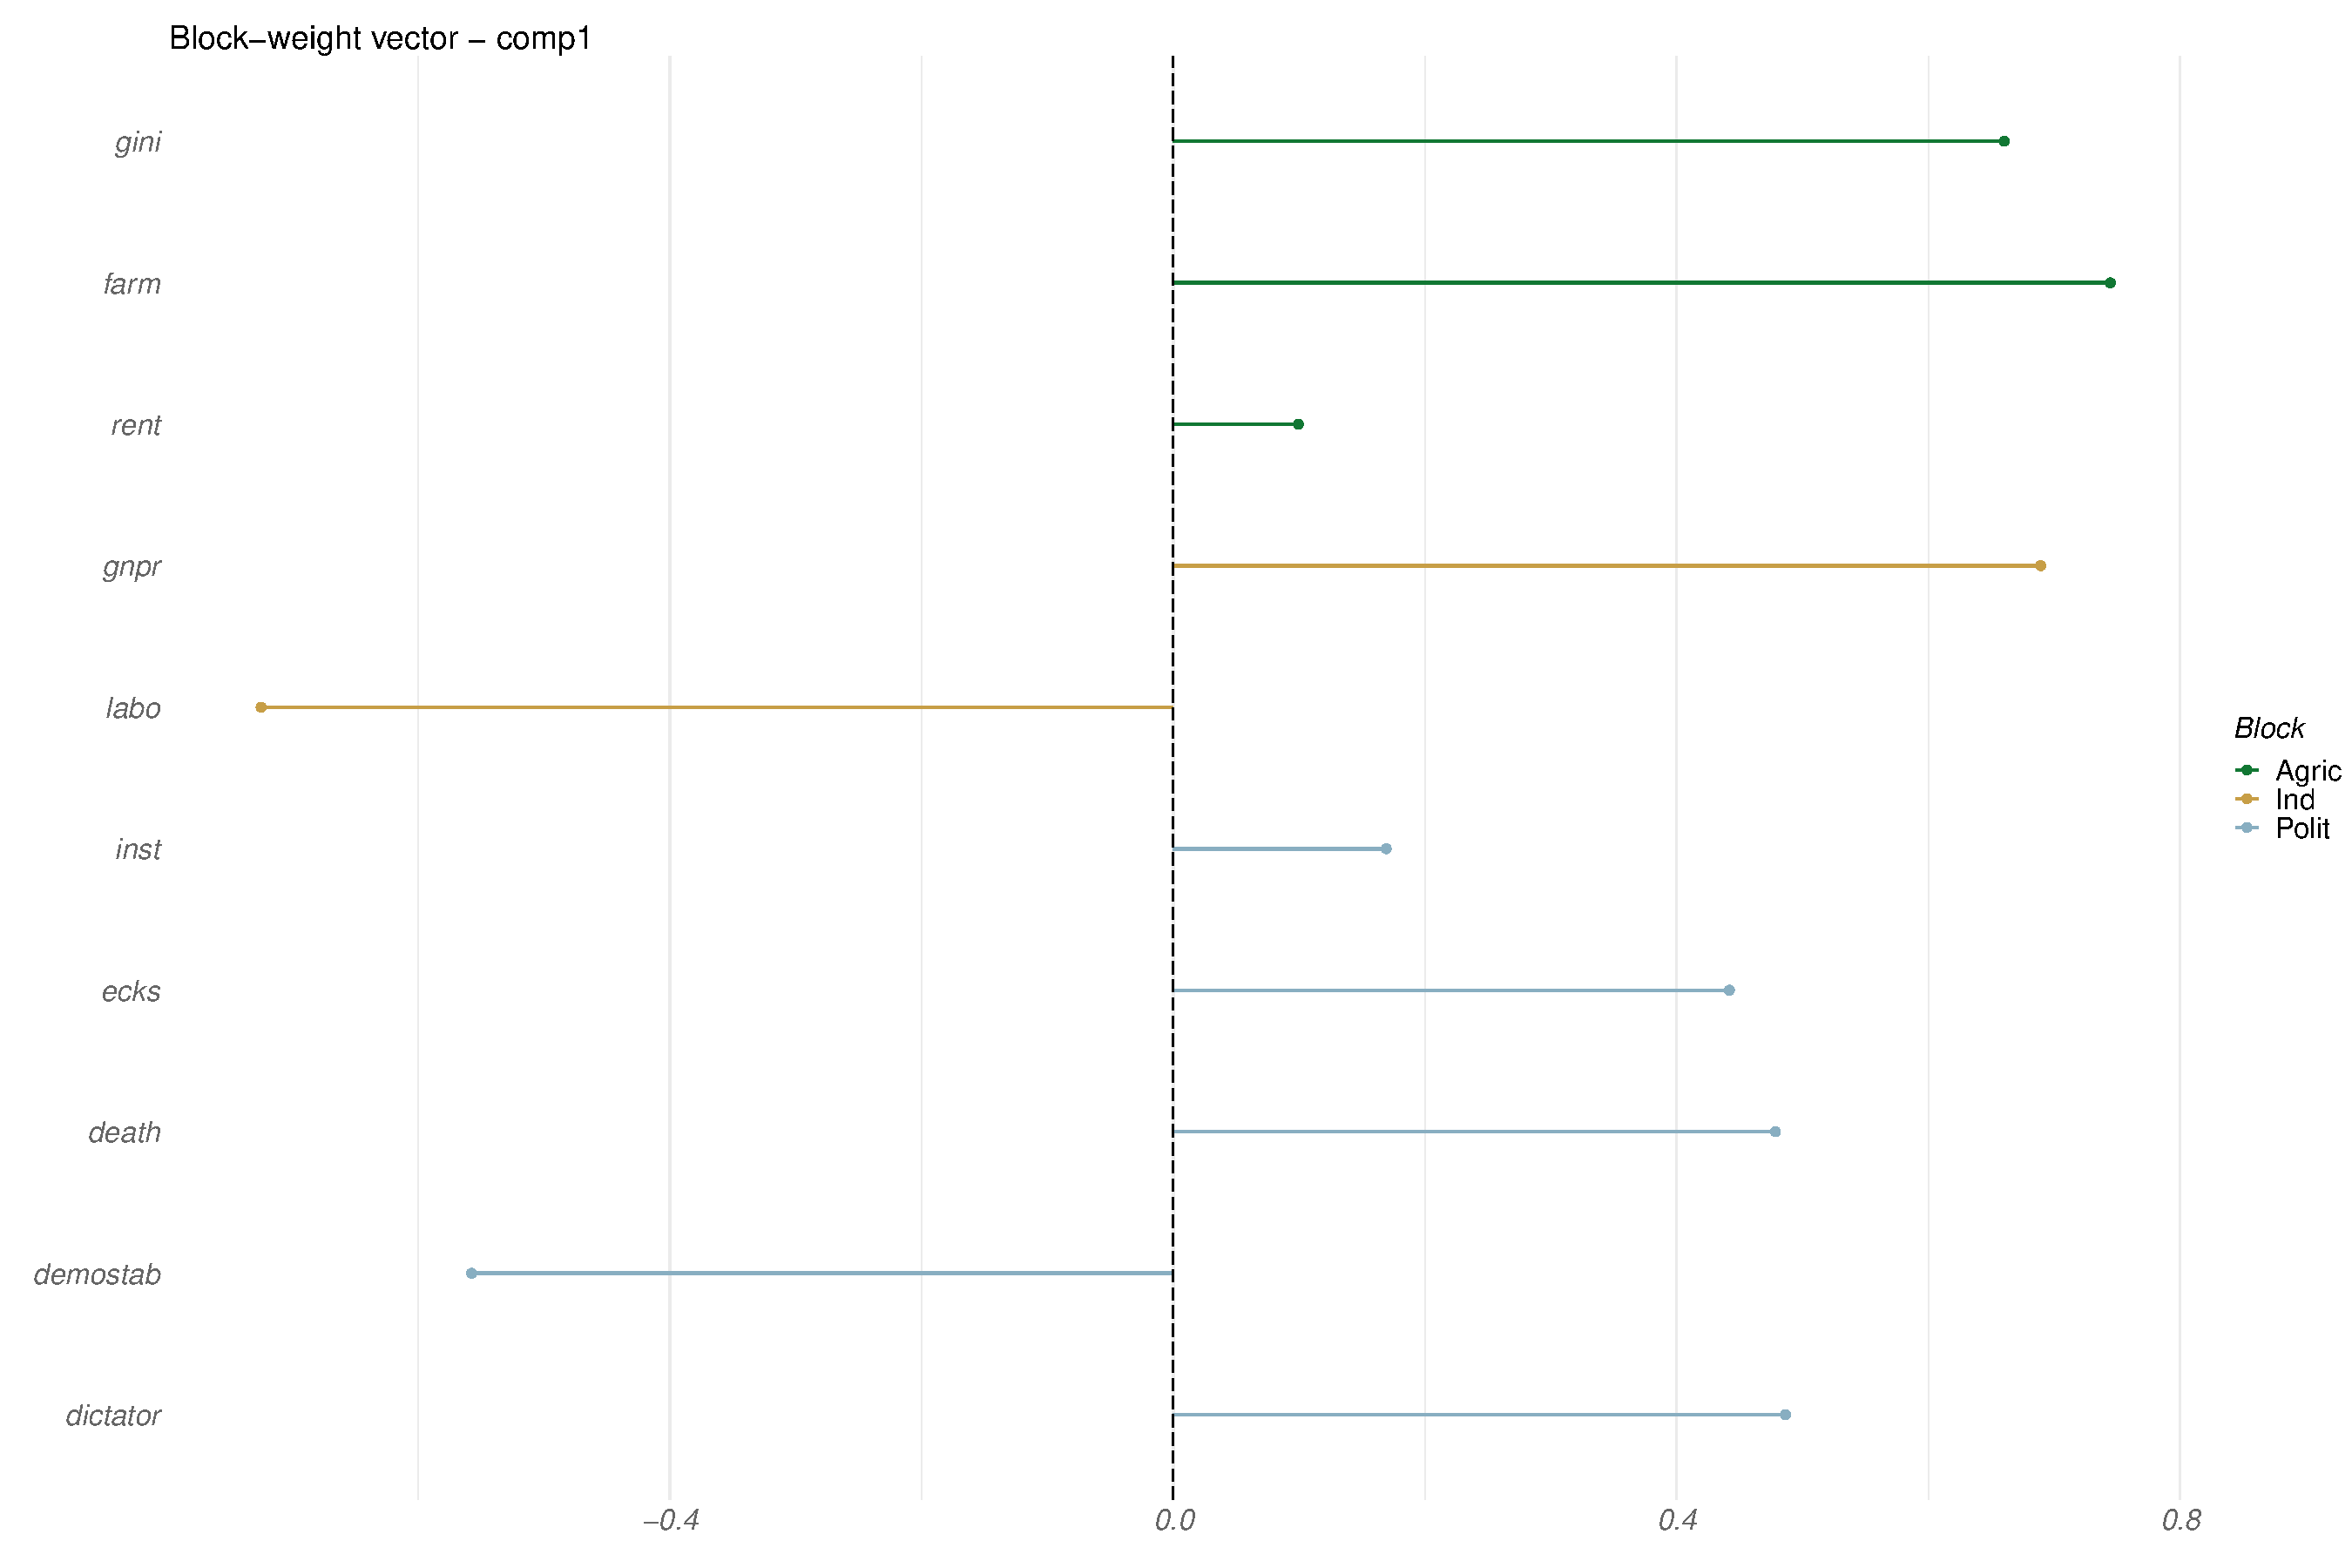
\includegraphics{RGCCA_files/figure-latex/unnamed-chunk-7-1} \end{center}

\end{CodeChunk}

\normalsize

\textbf{Assessment of the reliability of parameter estimates.} It is
possible to use a bootstrap resampling method to assess the reliability
of parameter estimates (block-weight/loading vectors) obtained using
RGCCA. \(B=\)\texttt{n\_boot} bootstrap samples of the same size as the
original data is repeatedly sampled with replacement from the original
data. RGCCA is then applied to each bootstrap sample to obtain the RGCCA
estimates. We calculate the standard deviation of the estimates across
the bootstrap samples, from which we derived, bootstrap confidence
intervals, t-ratio (defined as the ratio of the parameter estimate to
its bootstrap estimate of the standard deviation) and p-value (the
p-value is computed by assuming that the ratio of the parameter estimate
to its standard deviation follows the standardized normal distribution)
to indicate how reliably parameters were estimated. Since several
p-values are constructed simultaneously, FDR correction can be applied
for controlling the False Discovery Rate. This function is available
using the \texttt{rgcca\_bootstrap()} function of the RGCCA package.

\begin{CodeChunk}
\begin{CodeInput}
R> boot_out = rgcca_bootstrap(fit, n_boot = 500, n_cores = 1)
\end{CodeInput}
\begin{CodeOutput}
Bootstrap samples sanity check...OK
\end{CodeOutput}
\end{CodeChunk}

The bootstrap results are detailed using the \texttt{print()} function.

\footnotesize

\begin{CodeChunk}
\begin{CodeInput}
R> print(boot_out, block = 1:3, ncomp = 1)
\end{CodeInput}
\begin{CodeOutput}
Call: method='rgcca', superblock=FALSE, scale=TRUE, scale_block=FALSE, init='svd',
bias=TRUE, tol=1e-08, NA_method='nipals', ncomp=c(2,2,2), response=NULL,
comp_orth=TRUE 
There are J = 3 blocks.
The design matrix is:
      Agric Ind Polit
Agric     0   0     1
Ind       0   0     1
Polit     1   1     0

The factorial scheme is used.

Extracted statistics from 500 bootstrap samples.
Block-weight vectors for component 1: 
         estimate    mean     sd lower_bound upper_bound bootstrap_ratio   pval
gini       0.6602  0.6360 0.0773       0.426       0.734           8.540 0.0000
farm       0.7445  0.7318 0.0522       0.637       0.842          14.261 0.0000
rent       0.0994  0.0783 0.2128      -0.408       0.451           0.467 0.4006
gnpr       0.6891  0.6886 0.0325       0.612       0.743          21.222 0.0000
labo      -0.7247 -0.7237 0.0301      -0.791      -0.670         -24.108 0.0000
inst       0.1692  0.1681 0.1136      -0.065       0.355           1.489 0.0893
ecks       0.4418  0.4352 0.0621       0.315       0.546           7.120 0.0000
death      0.4784  0.4705 0.0515       0.363       0.567           9.296 0.0000
demostab  -0.5574 -0.5505 0.0503      -0.644      -0.438         -11.086 0.0000
dictator   0.4864  0.4828 0.0538       0.363       0.584           9.045 0.0000
         adjust.pval
gini           0.000
farm           0.000
rent           0.471
gnpr           0.000
labo           0.000
inst           0.128
ecks           0.000
death          0.000
demostab       0.000
dictator       0.000
\end{CodeOutput}
\end{CodeChunk}

\normalsize

and displayed using the \texttt{plot()}function.

\footnotesize

\begin{CodeChunk}
\begin{CodeInput}
R> plot(boot_out, type = "weight", 
+      block = 1:3, comp = 1, 
+      display_order = FALSE, cex = 1.3)
\end{CodeInput}


\begin{center}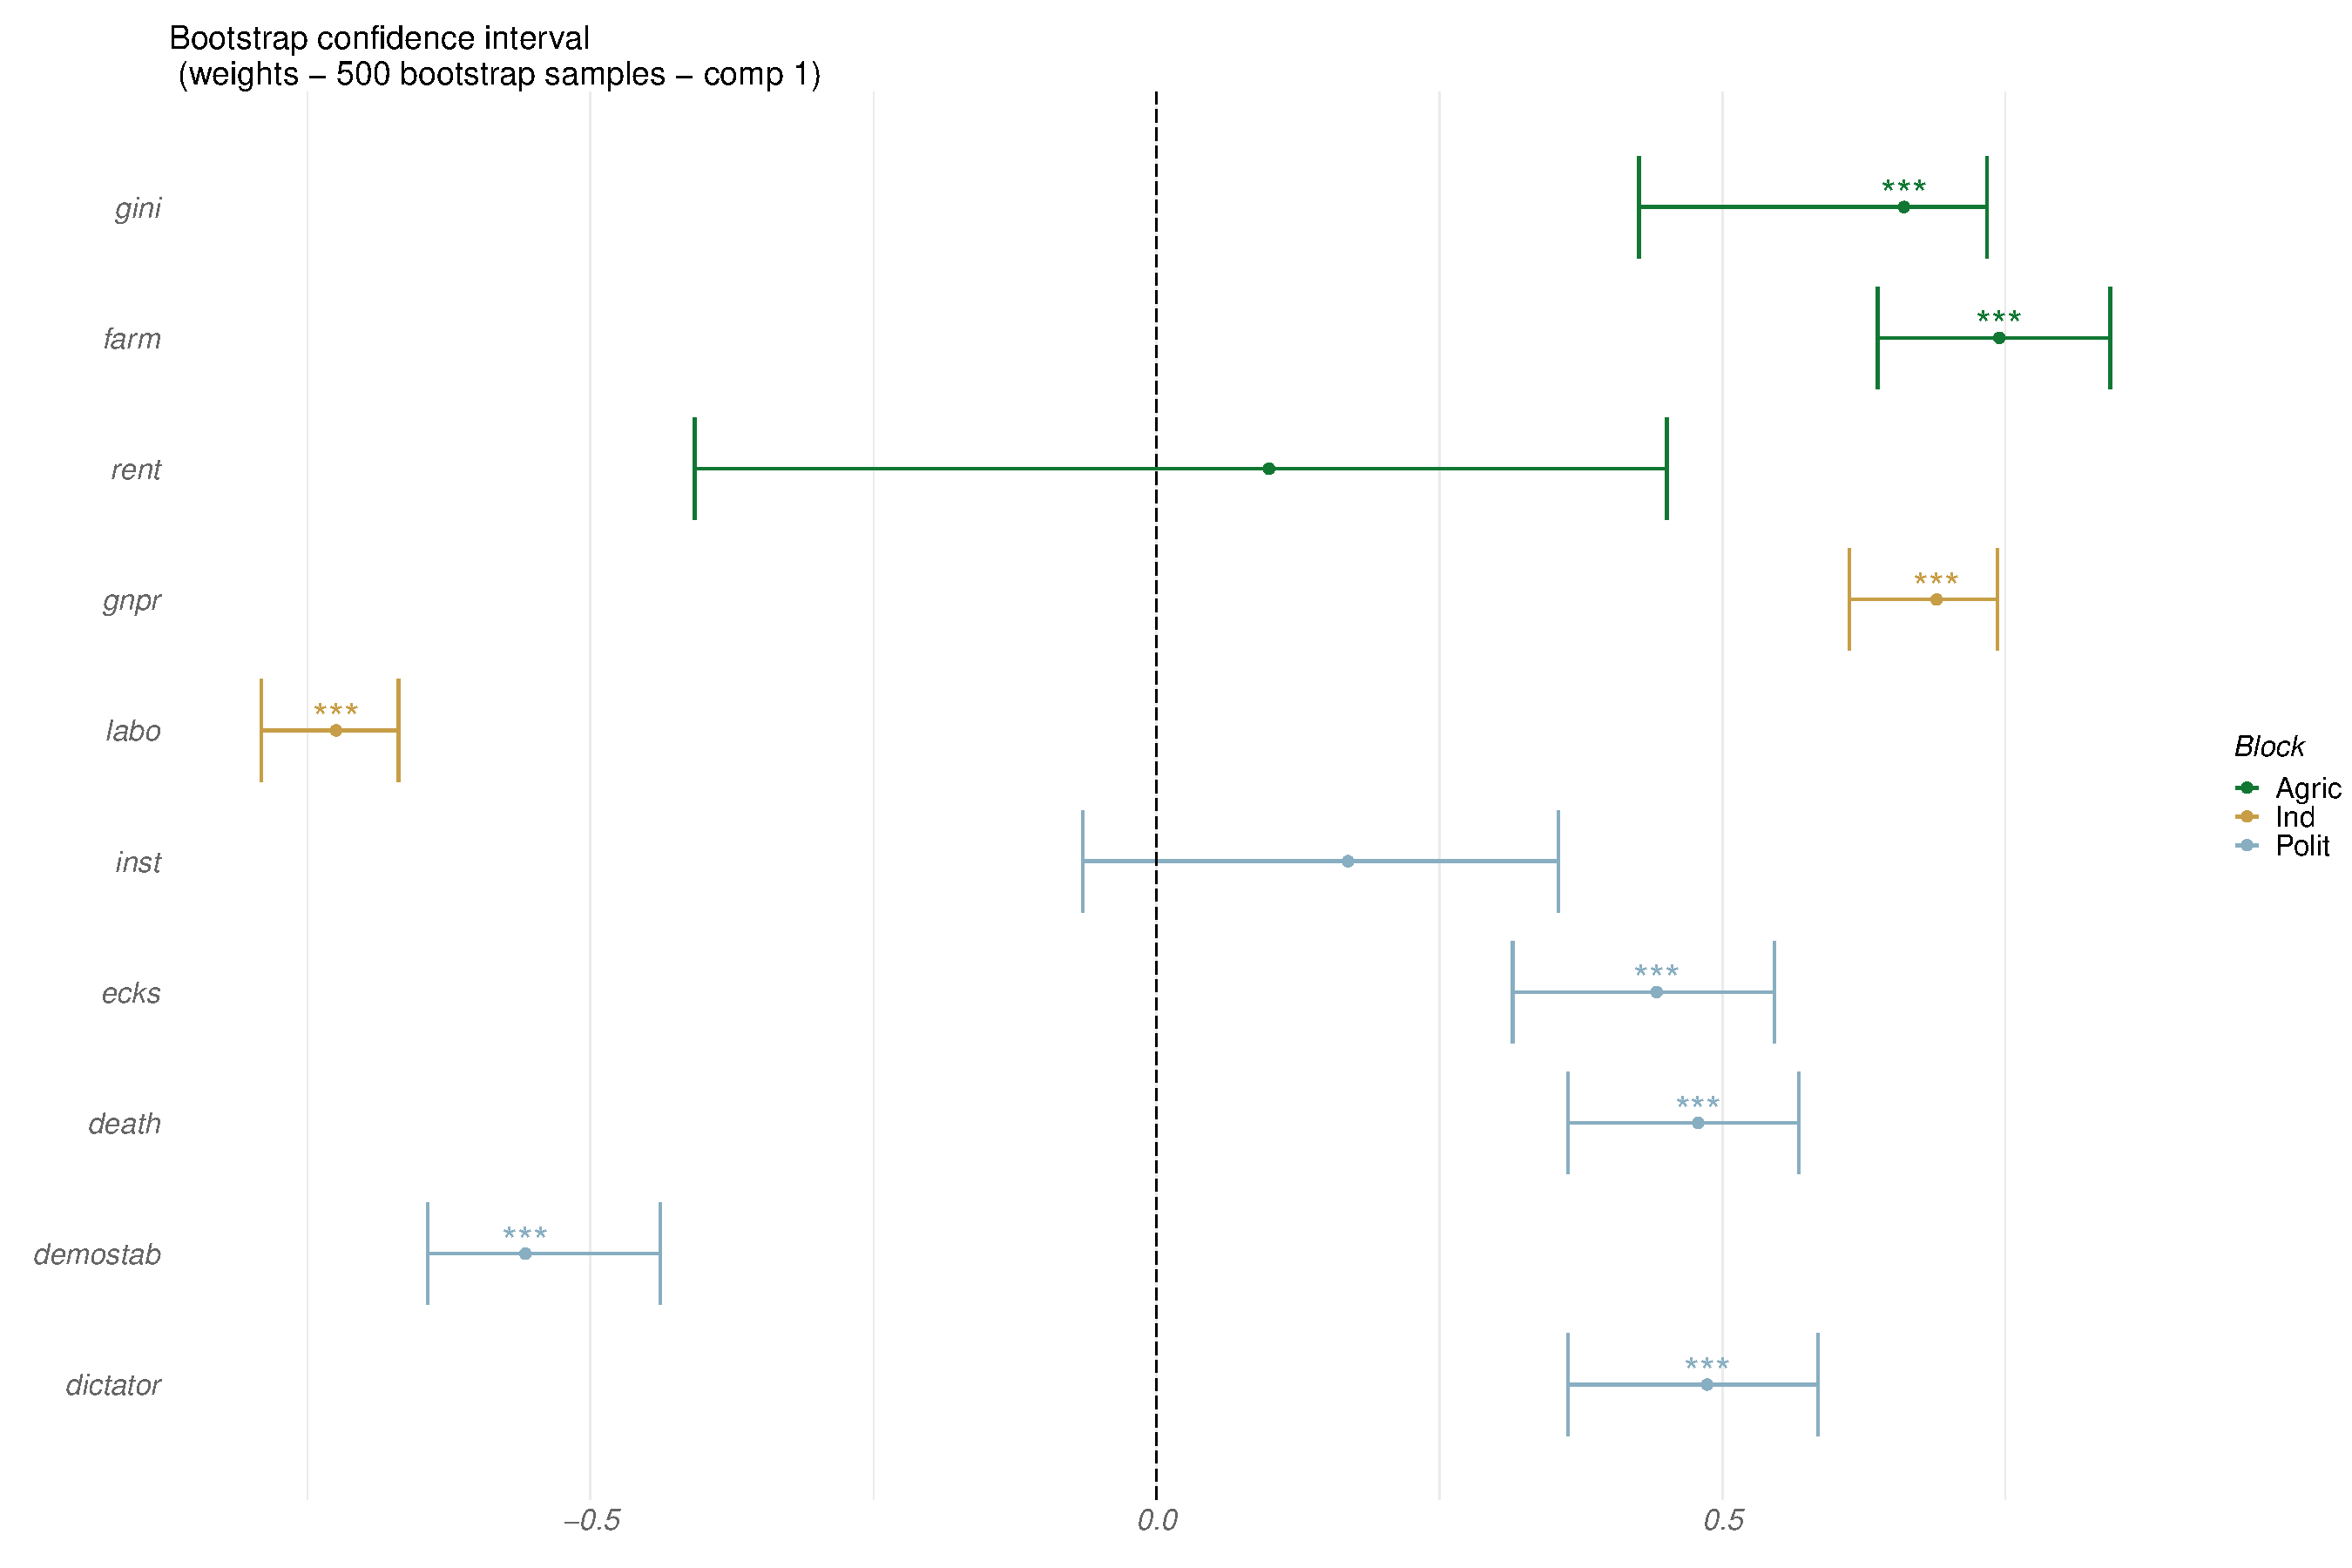
\includegraphics{RGCCA_files/figure-latex/unnamed-chunk-10-1} \end{center}

\end{CodeChunk}

\normalsize

At last, as a component-based method, The RGCCA package provides block
components as output of the \texttt{rgcca()} function in \texttt{fit\$Y}
and graphical representations, including factor plot and correlation
circle. This graphical displays allows visualizing the sources of
variability within blocks, the relationships between variables within
and between blocks and the amount of correlation between blocks. The
graphical display of the countries obtained by crossing
\(\ensuremath{\mathbf{X}}_1 \ensuremath{\mathbf{a}}_1\) = Agricultural
Inequality and \(\ensuremath{\mathbf{X}}_2 \ensuremath{\mathbf{a}}_2\) =
Industrial Development and marked with their political regime in 1960 is
shown in below.

\footnotesize

\begin{CodeChunk}
\begin{CodeInput}
R> plot(fit, type = "sample",
+      block = 1:2, comp = 1,
+      resp = lab, repel = TRUE, cex = 1.3)
\end{CodeInput}
\begin{figure}

{\centering 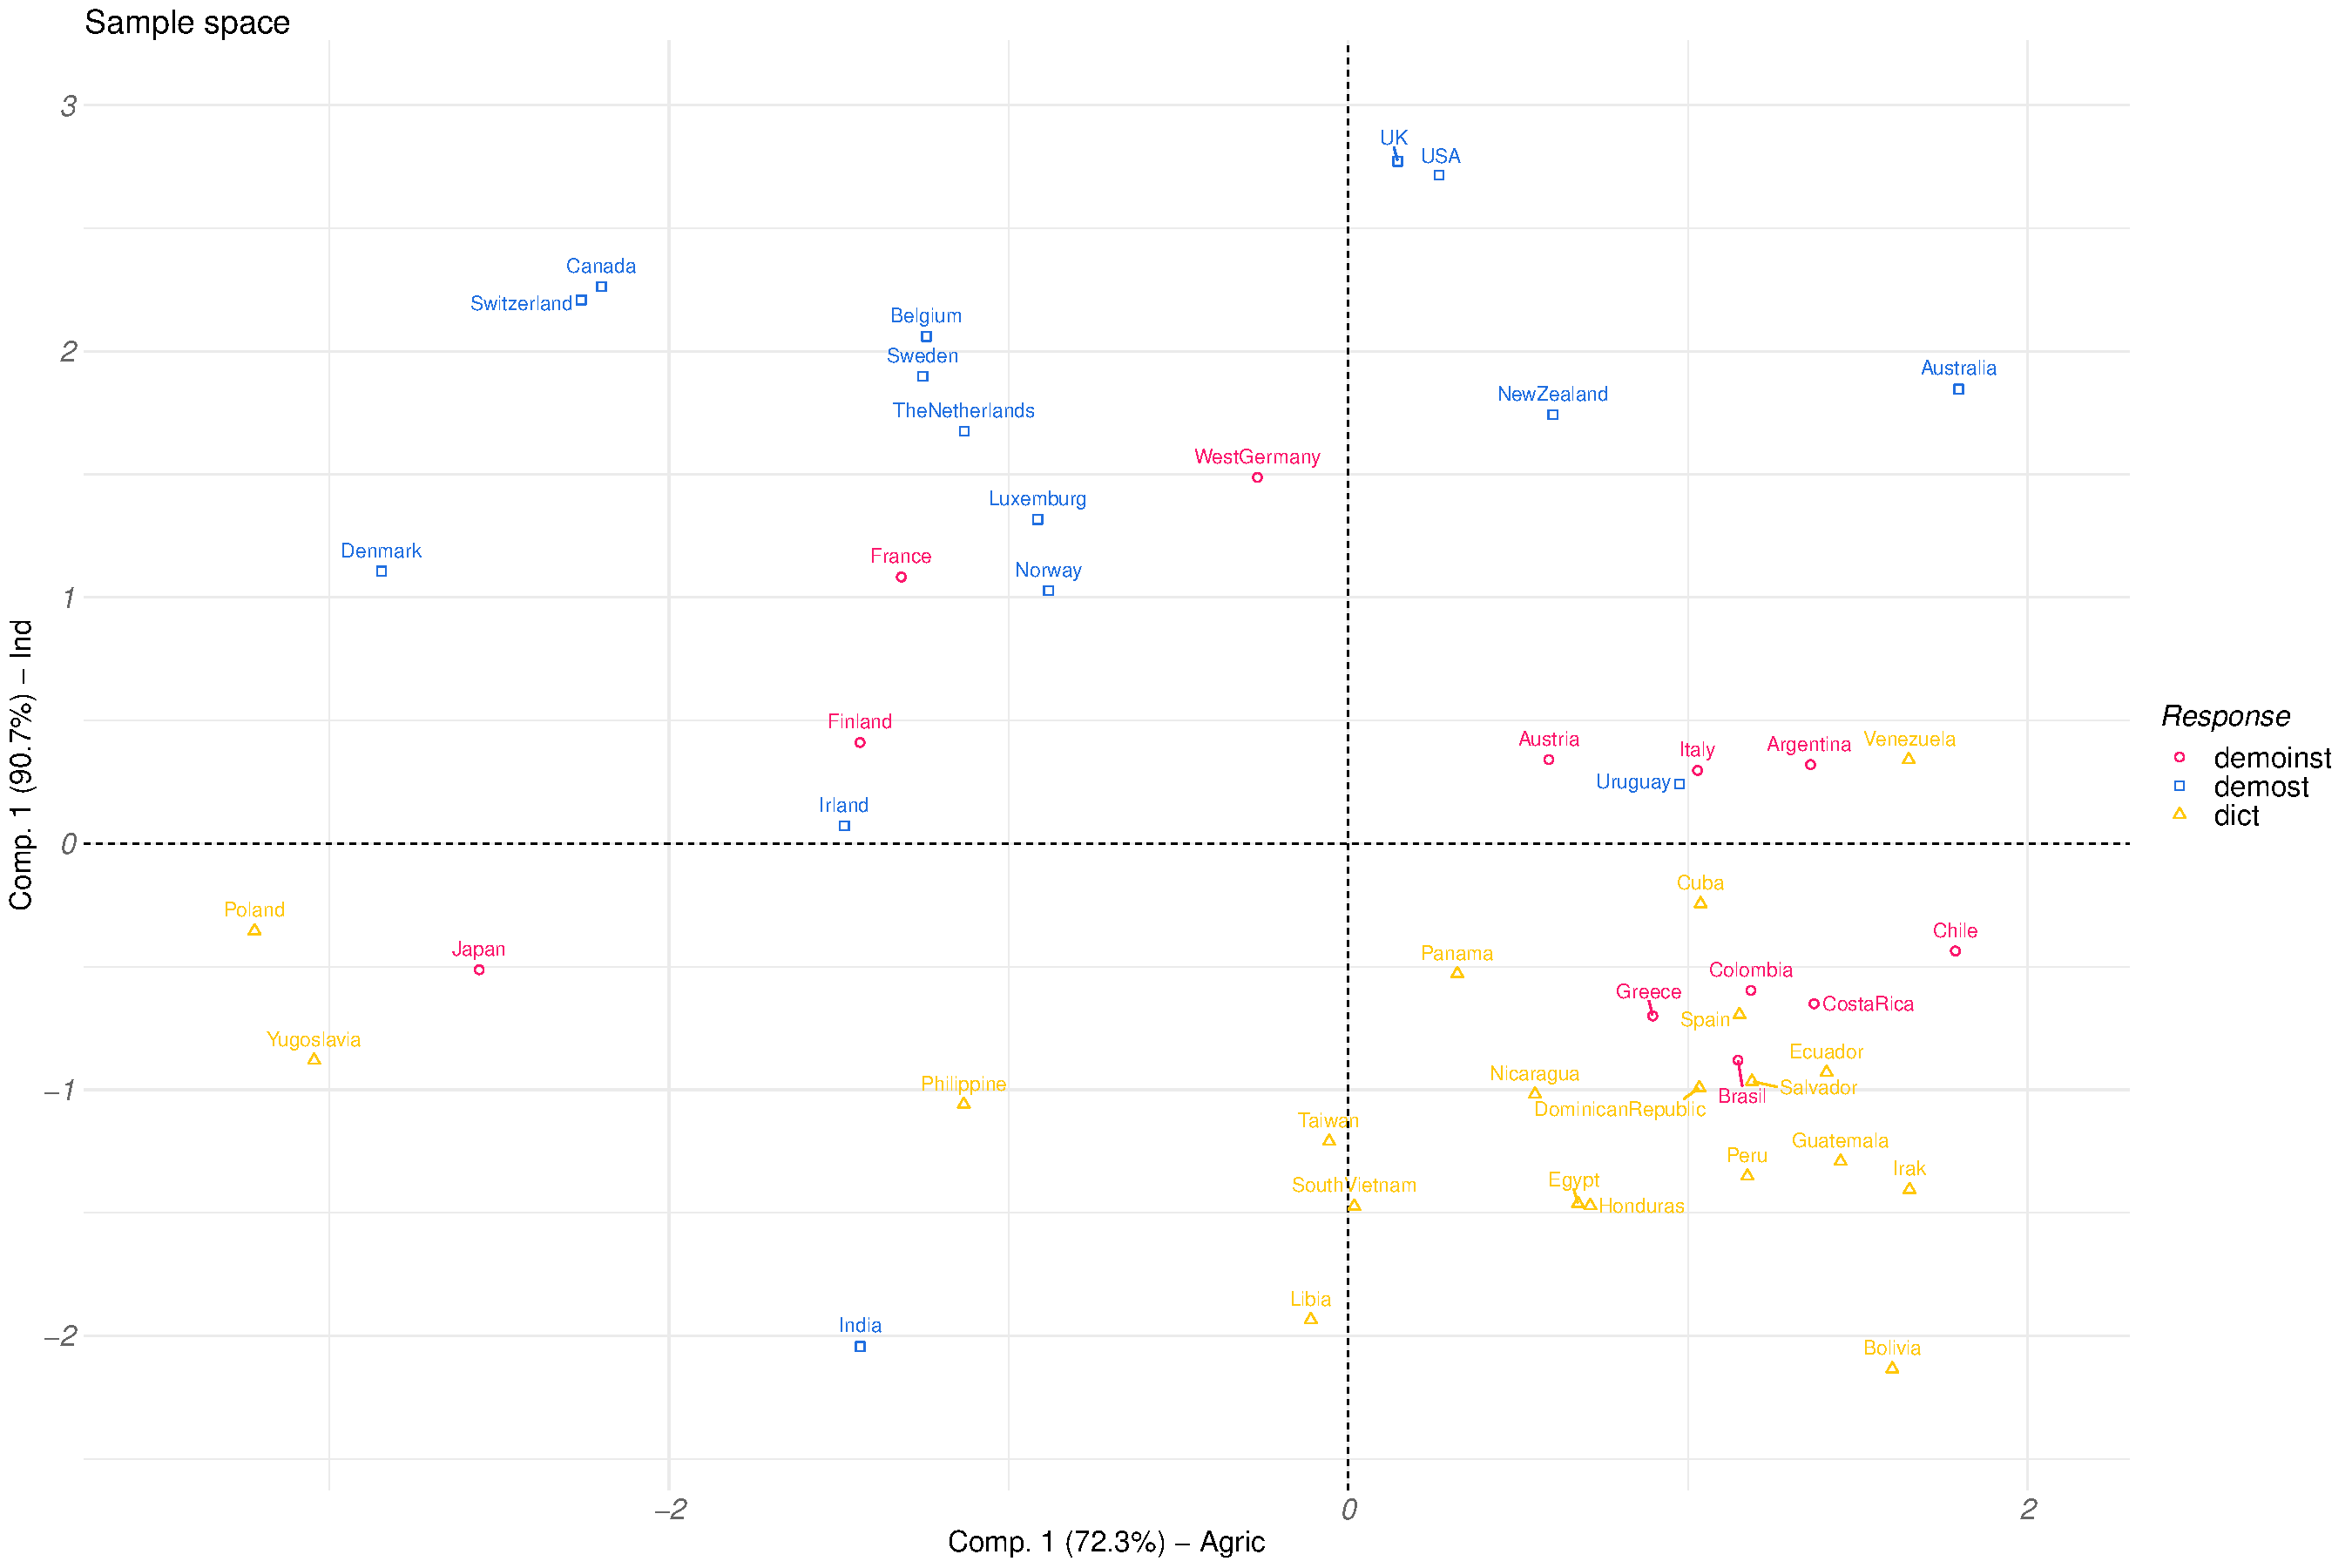
\includegraphics{RGCCA_files/figure-latex/unnamed-chunk-11-1} 

}

\caption[graphical display of the countries obtained by crossing y11 and y21 and labeled according to their political regime]{graphical display of the countries obtained by crossing y11 and y21 and labeled according to their political regime}\label{fig:unnamed-chunk-11}
\end{figure}
\end{CodeChunk}

\normalsize

Countries aggregate together when they share similarities. It may be
noted that the lower ight quadrant concentrates on dictatorships. It is
difficult for a country to escape dictatorship when its industrial
development is below-average and its agricultural inequality is above
average. It is worth pointing out that some unstable democracies located
in this quadrant (or close to it) became dictatorships for a period of
time after 1960: Greece (1967-1974), Brazil (1964-1985), Chili
(1973-1990), and Argentina (1966-1973). The Average Variance Explained
(AVE) defined below is also reported in the axis of the Figure. The AVE
of block \(\mathbf{X}_j\) for a specific block component
\(\mathbf{y}_j\) is defined as:

\begin{equation}
\mathrm{AVE}({\mathbf{X}_j)=  \frac{1}{\Vert \mathbf{X}_j \Vert^2} \sum_{h=1}^{p_j} var(\mathbf{x}_{jh}) \times cor^2( \mathbf{x}}_{jh},\mathbf{y}_j)
\end{equation}

AVE(\(\mathbf{X}_j\)) varies between 0 and 1 and reflects the proportion
of variance captured by \(\mathbf{y}_j\).

Additional indicators of model quality are also proposed:

\begin{itemize}
\tightlist
\item
  For all blocks:
\end{itemize}

\begin{equation}
\displaystyle \mathrm{AVE(outer model)} = \left( 1/\sum_j p_j \right) \sum_j p_j \mathrm{AVE}(\ensuremath{\mathbf{X}}_j)
\end{equation}

\begin{itemize}
\tightlist
\item
  For the inner model:
\end{itemize}

\begin{equation}
\displaystyle \mathrm{AVE(inner model)} = \left( 1/\sum_{j<k} c_{jk} \right) \sum_{j<k} c_{jk} \mathrm{cor}^2(\ensuremath{\mathbf{y}}_j , \ensuremath{\mathbf{y}}_k)
\end{equation}

These indicators of model quality are also available as output of the
\texttt{rgcca()} function in \texttt{fit\$AVE}. These AVEs can be
visualized using the generic \texttt{plot()} function.

\footnotesize

\begin{CodeChunk}
\begin{CodeInput}
R> plot(fit, type = "ave", cex = 1.3)
\end{CodeInput}
\begin{figure}

{\centering 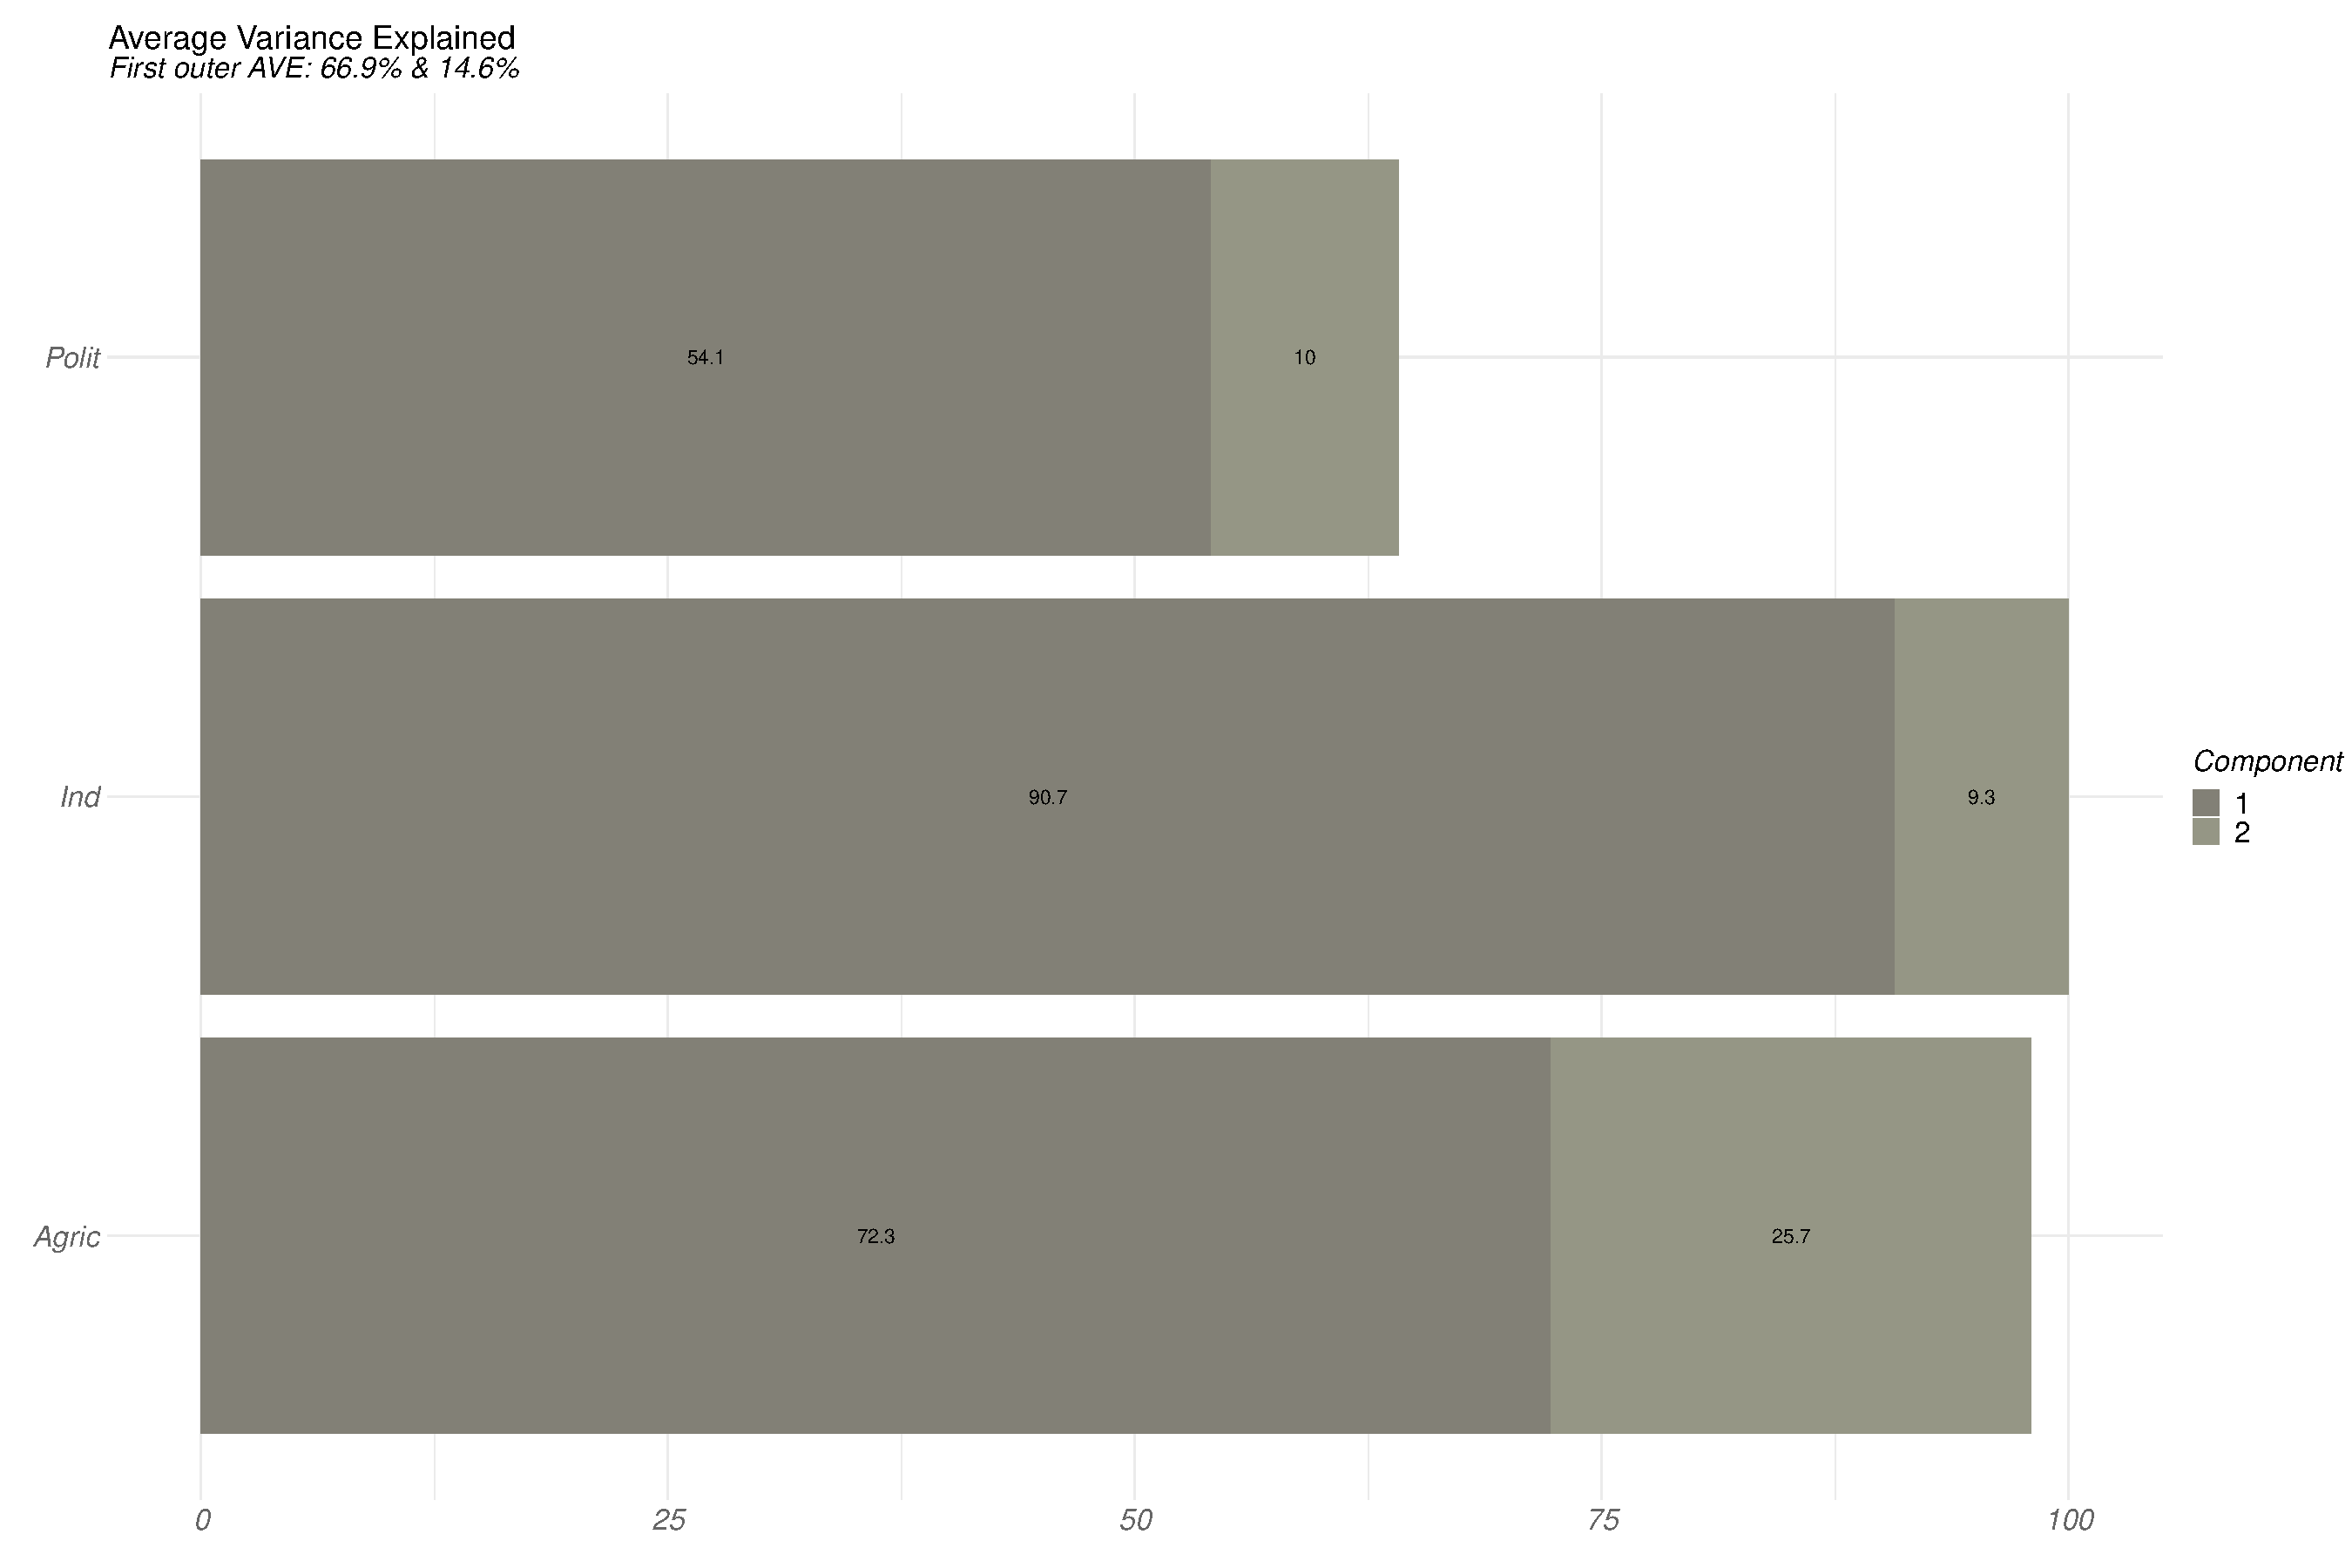
\includegraphics{RGCCA_files/figure-latex/unnamed-chunk-12-1} 

}

\caption[Average variance explained of the various blocks]{Average variance explained of the various blocks}\label{fig:unnamed-chunk-12}
\end{figure}
\end{CodeChunk}

\normalsize

\hypertarget{rgcca-with-superblock}{%
\subsection{RGCCA with superblock}\label{rgcca-with-superblock}}

When the superblock option is considered global components can be
derived. The space spanned by the global components can be viewed as a
consensus space that integrated all the modalities and facilitates the
visualization of the results and their interpretation. In this section,
we consider Multiple Co-Inertia Analysis \cite{Hanafi2006} with \(2\)
components per block. See \texttt{available\_methods()} for a list of
pre-specified multiblock component methods.

\footnotesize

\begin{CodeChunk}
\begin{CodeInput}
R> fit.mcoa = rgcca(blocks=A, method = "mcoa", ncomp = 2)
\end{CodeInput}
\end{CodeChunk}

\normalsize

MCOA enables the countries to be represented in the space spanned by the
two first global components. Despite some overlap, the first global
component exhibits a separation/continuum among regimes.

\footnotesize

\begin{CodeChunk}
\begin{CodeInput}
R> plot(fit.mcoa, type = "sample", 
+      block = 4, comp = 1:2, 
+      response = lab, repel = TRUE, cex = 1.3)
\end{CodeInput}
\begin{figure}

{\centering 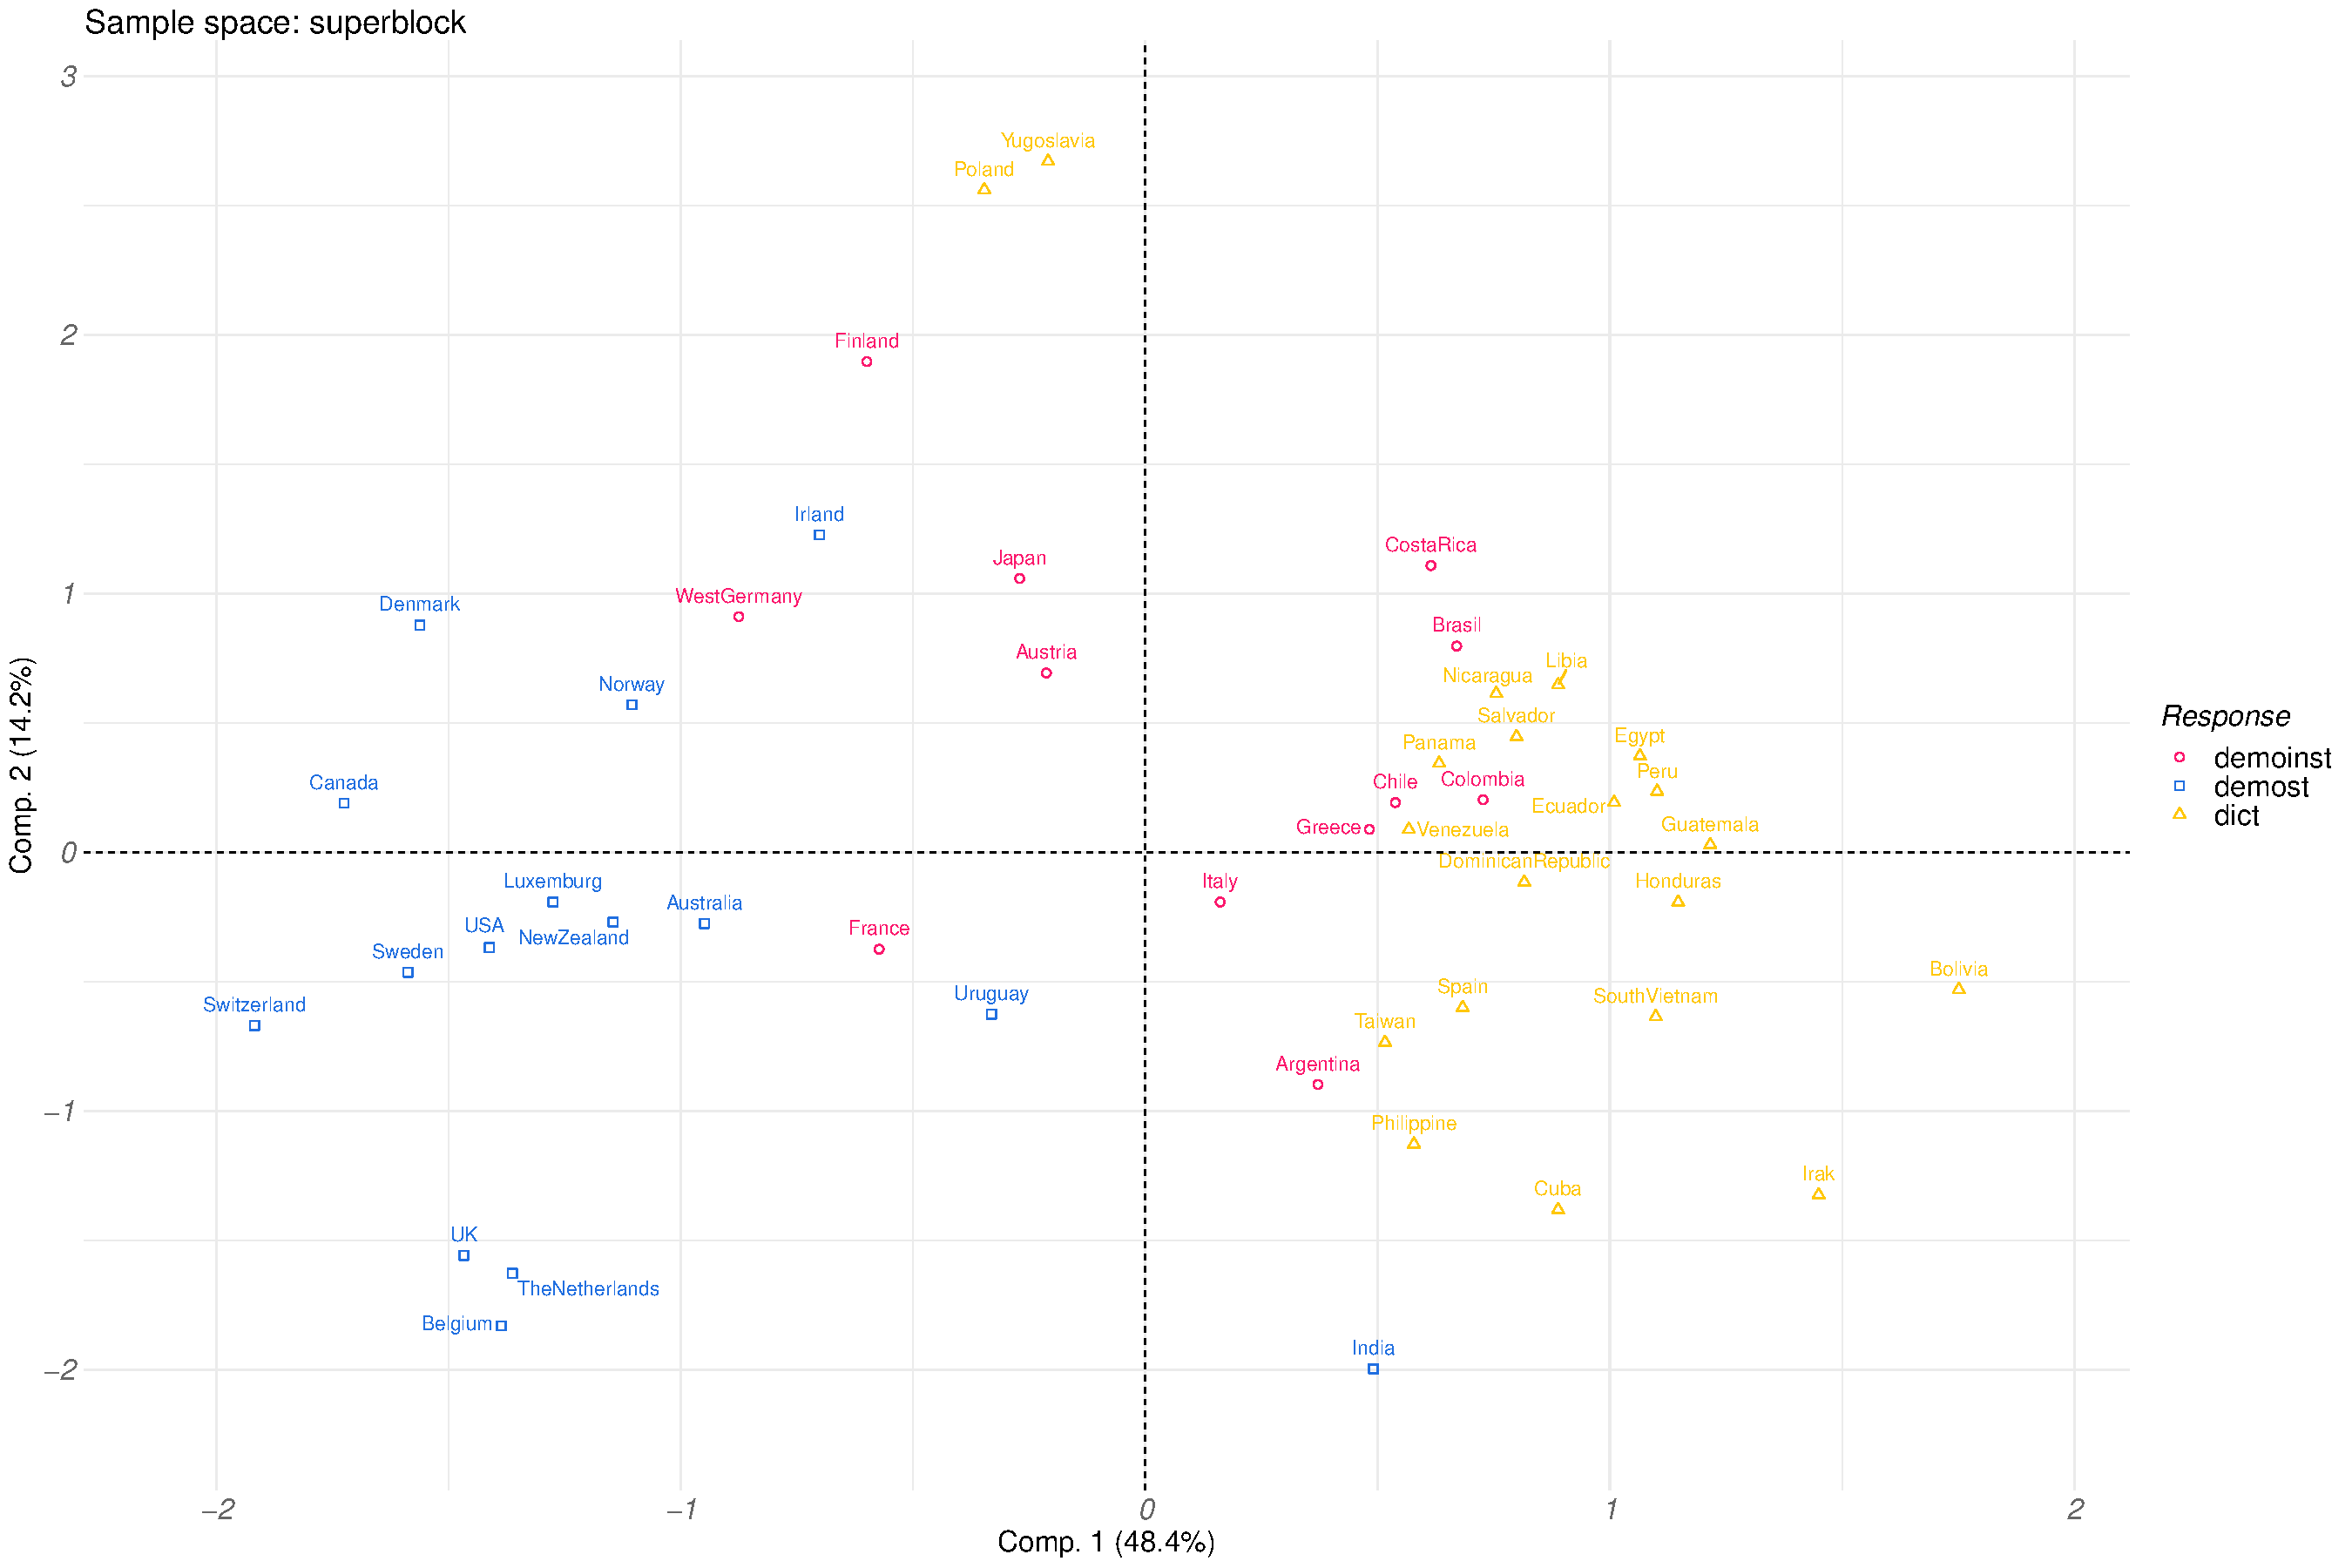
\includegraphics{RGCCA_files/figure-latex/unnamed-chunk-14-1} 

}

\caption[graphical display of the countries obtained by crossing the two first components of the superblock and labeled according to their political regime]{graphical display of the countries obtained by crossing the two first components of the superblock and labeled according to their political regime}\label{fig:unnamed-chunk-14}
\end{figure}
\end{CodeChunk}

\normalsize

Moreover, the correlation circle highlights the contribution of each
variable to the construction of the global components.

\footnotesize

\begin{CodeChunk}
\begin{CodeInput}
R> plot(fit.mcoa, type = "cor_circle",
+      block = 4, comp = 1:2, 
+      repel = TRUE, cex = 1.3)
\end{CodeInput}
\begin{figure}

{\centering 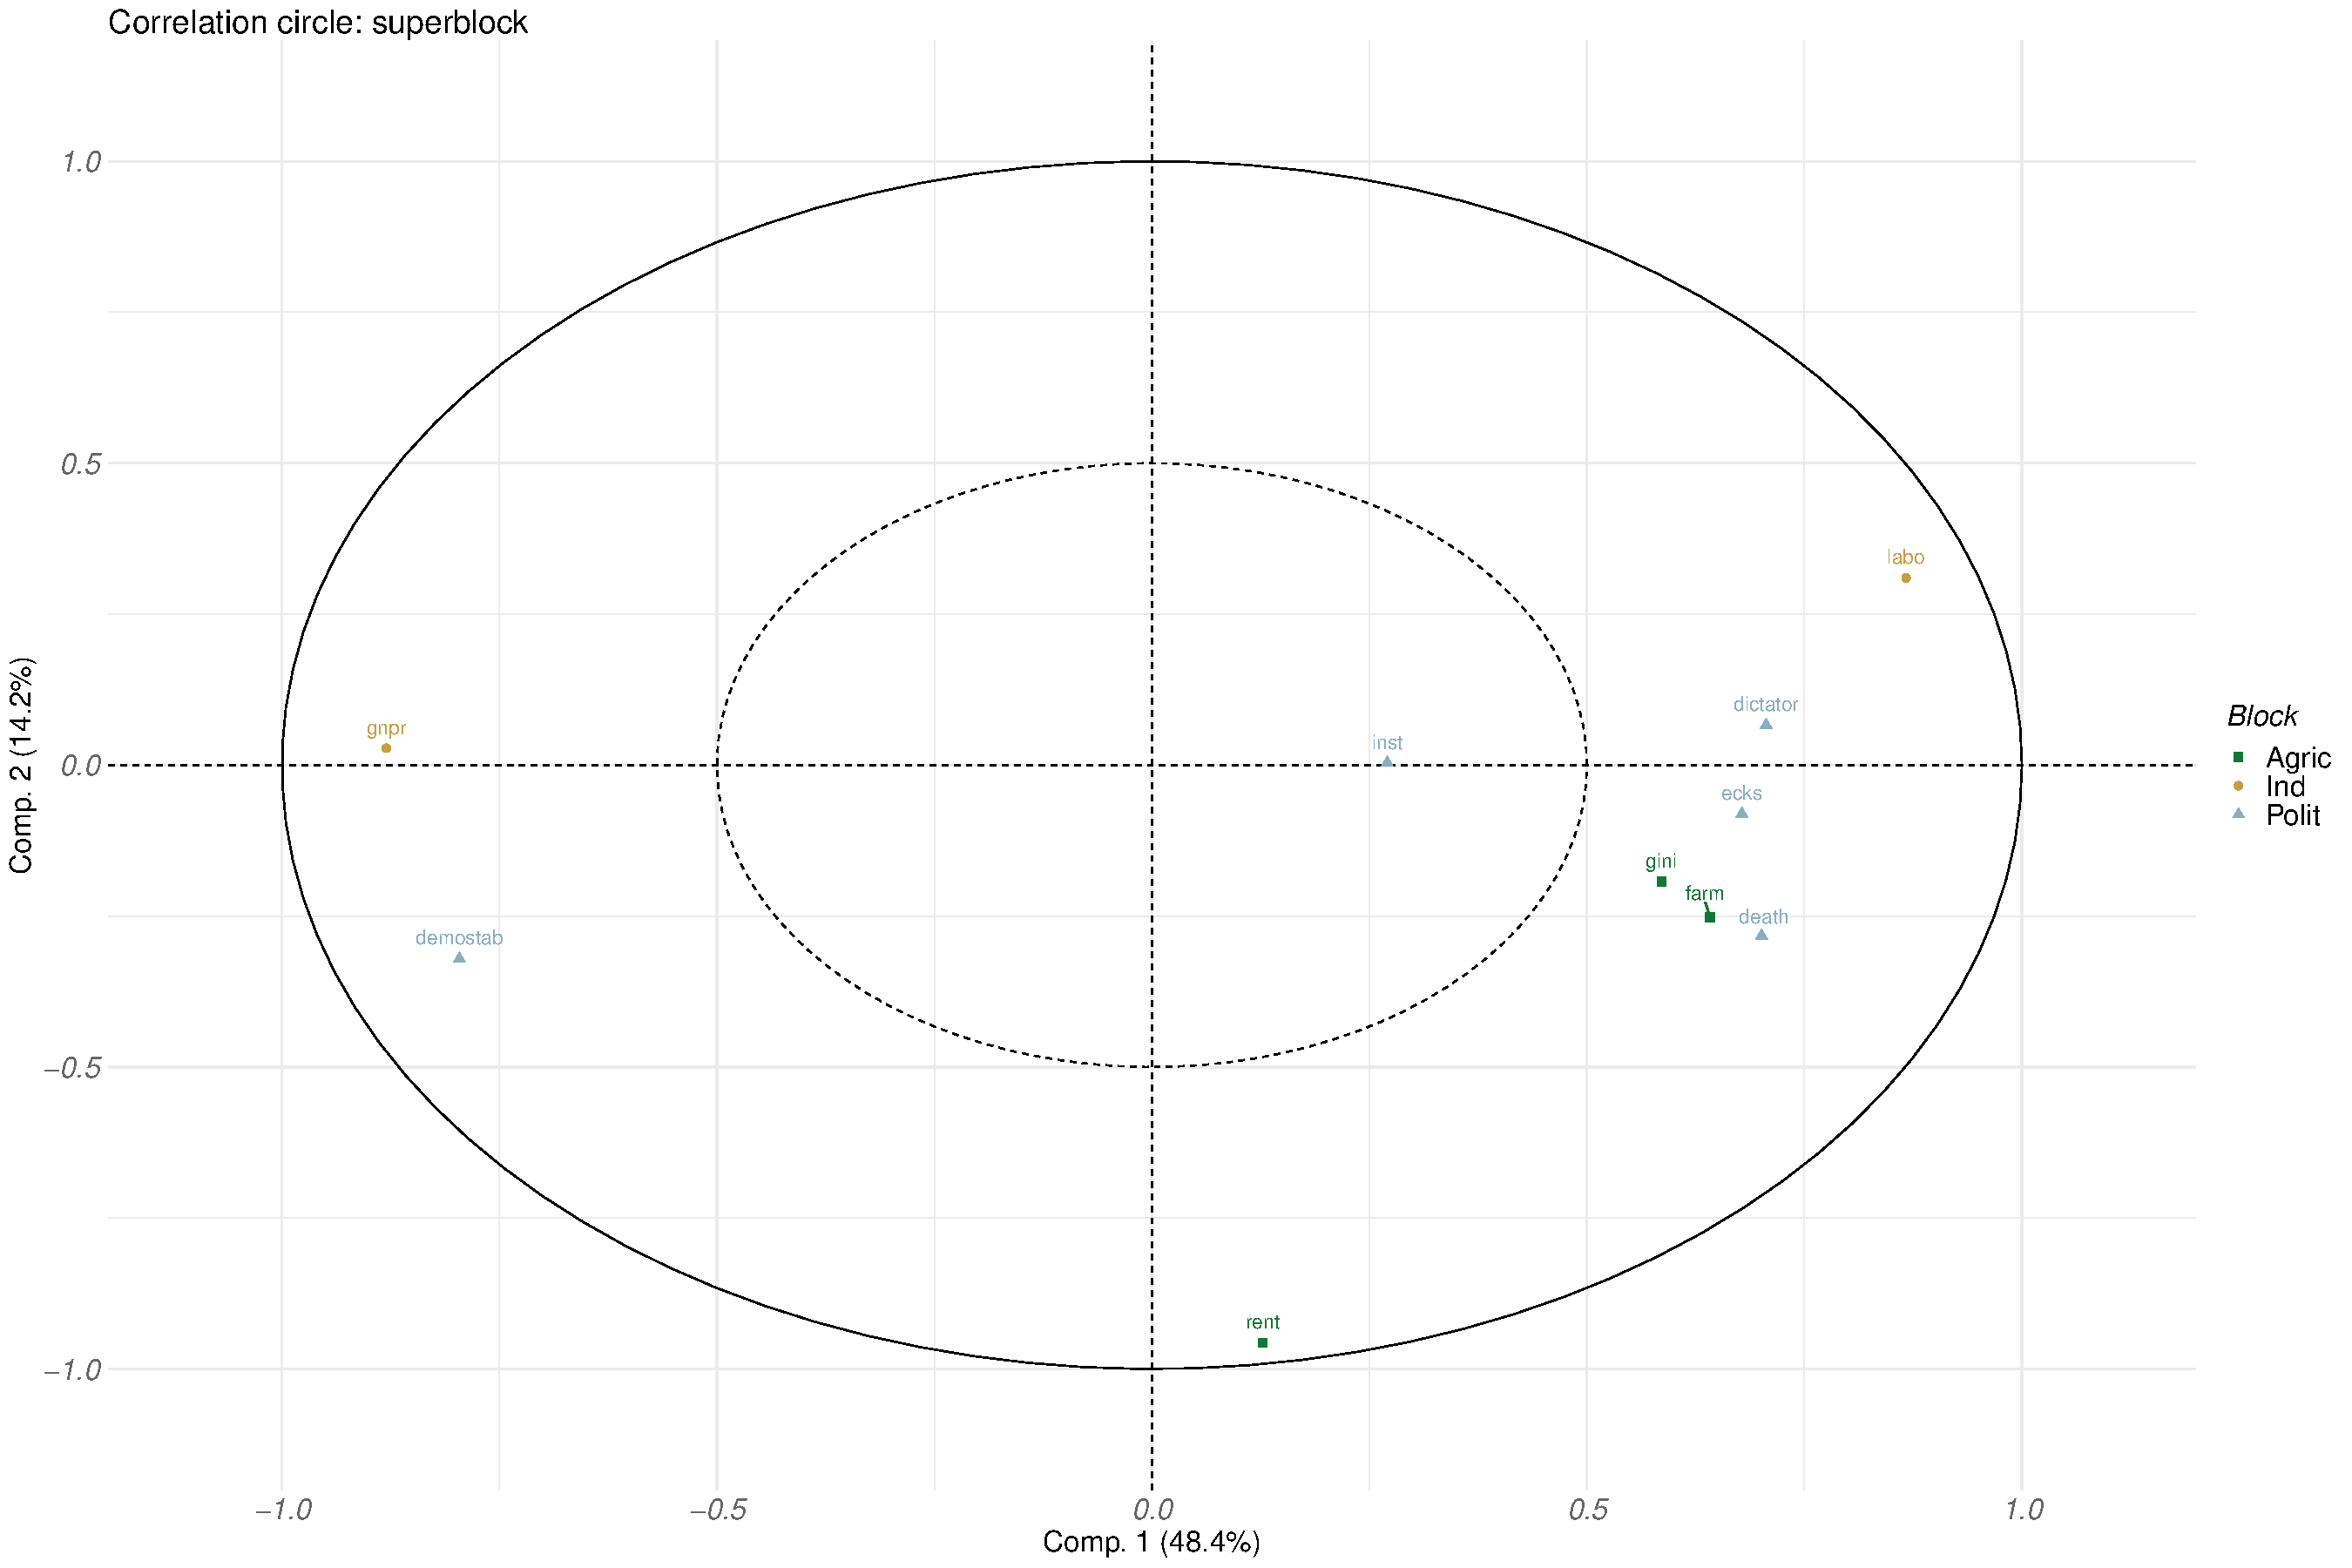
\includegraphics{RGCCA_files/figure-latex/unnamed-chunk-15-1} 

}

\caption[graphical display of the correlation cicle associated with the two first components of the superblock]{graphical display of the correlation cicle associated with the two first components of the superblock. Each variable are colored according to their block membership}\label{fig:unnamed-chunk-15}
\end{figure}
\end{CodeChunk}

\normalsize

A variable that is highly expressed for a category of individuals is
projected with a high weight (far from the origin) in the direction of
that category.

It is often useful to visualize jointly the sample space and the
correlation circle. This is make possible by using the
\texttt{type\ =\ "both"} argument of the plot function.

\footnotesize

\begin{CodeChunk}
\begin{CodeInput}
R> plot(fit.mcoa, type = "both",
+      block = 4, comp = 1:2, 
+      repel = TRUE, cex = 1.3, response = lab)
\end{CodeInput}
\begin{figure}

{\centering 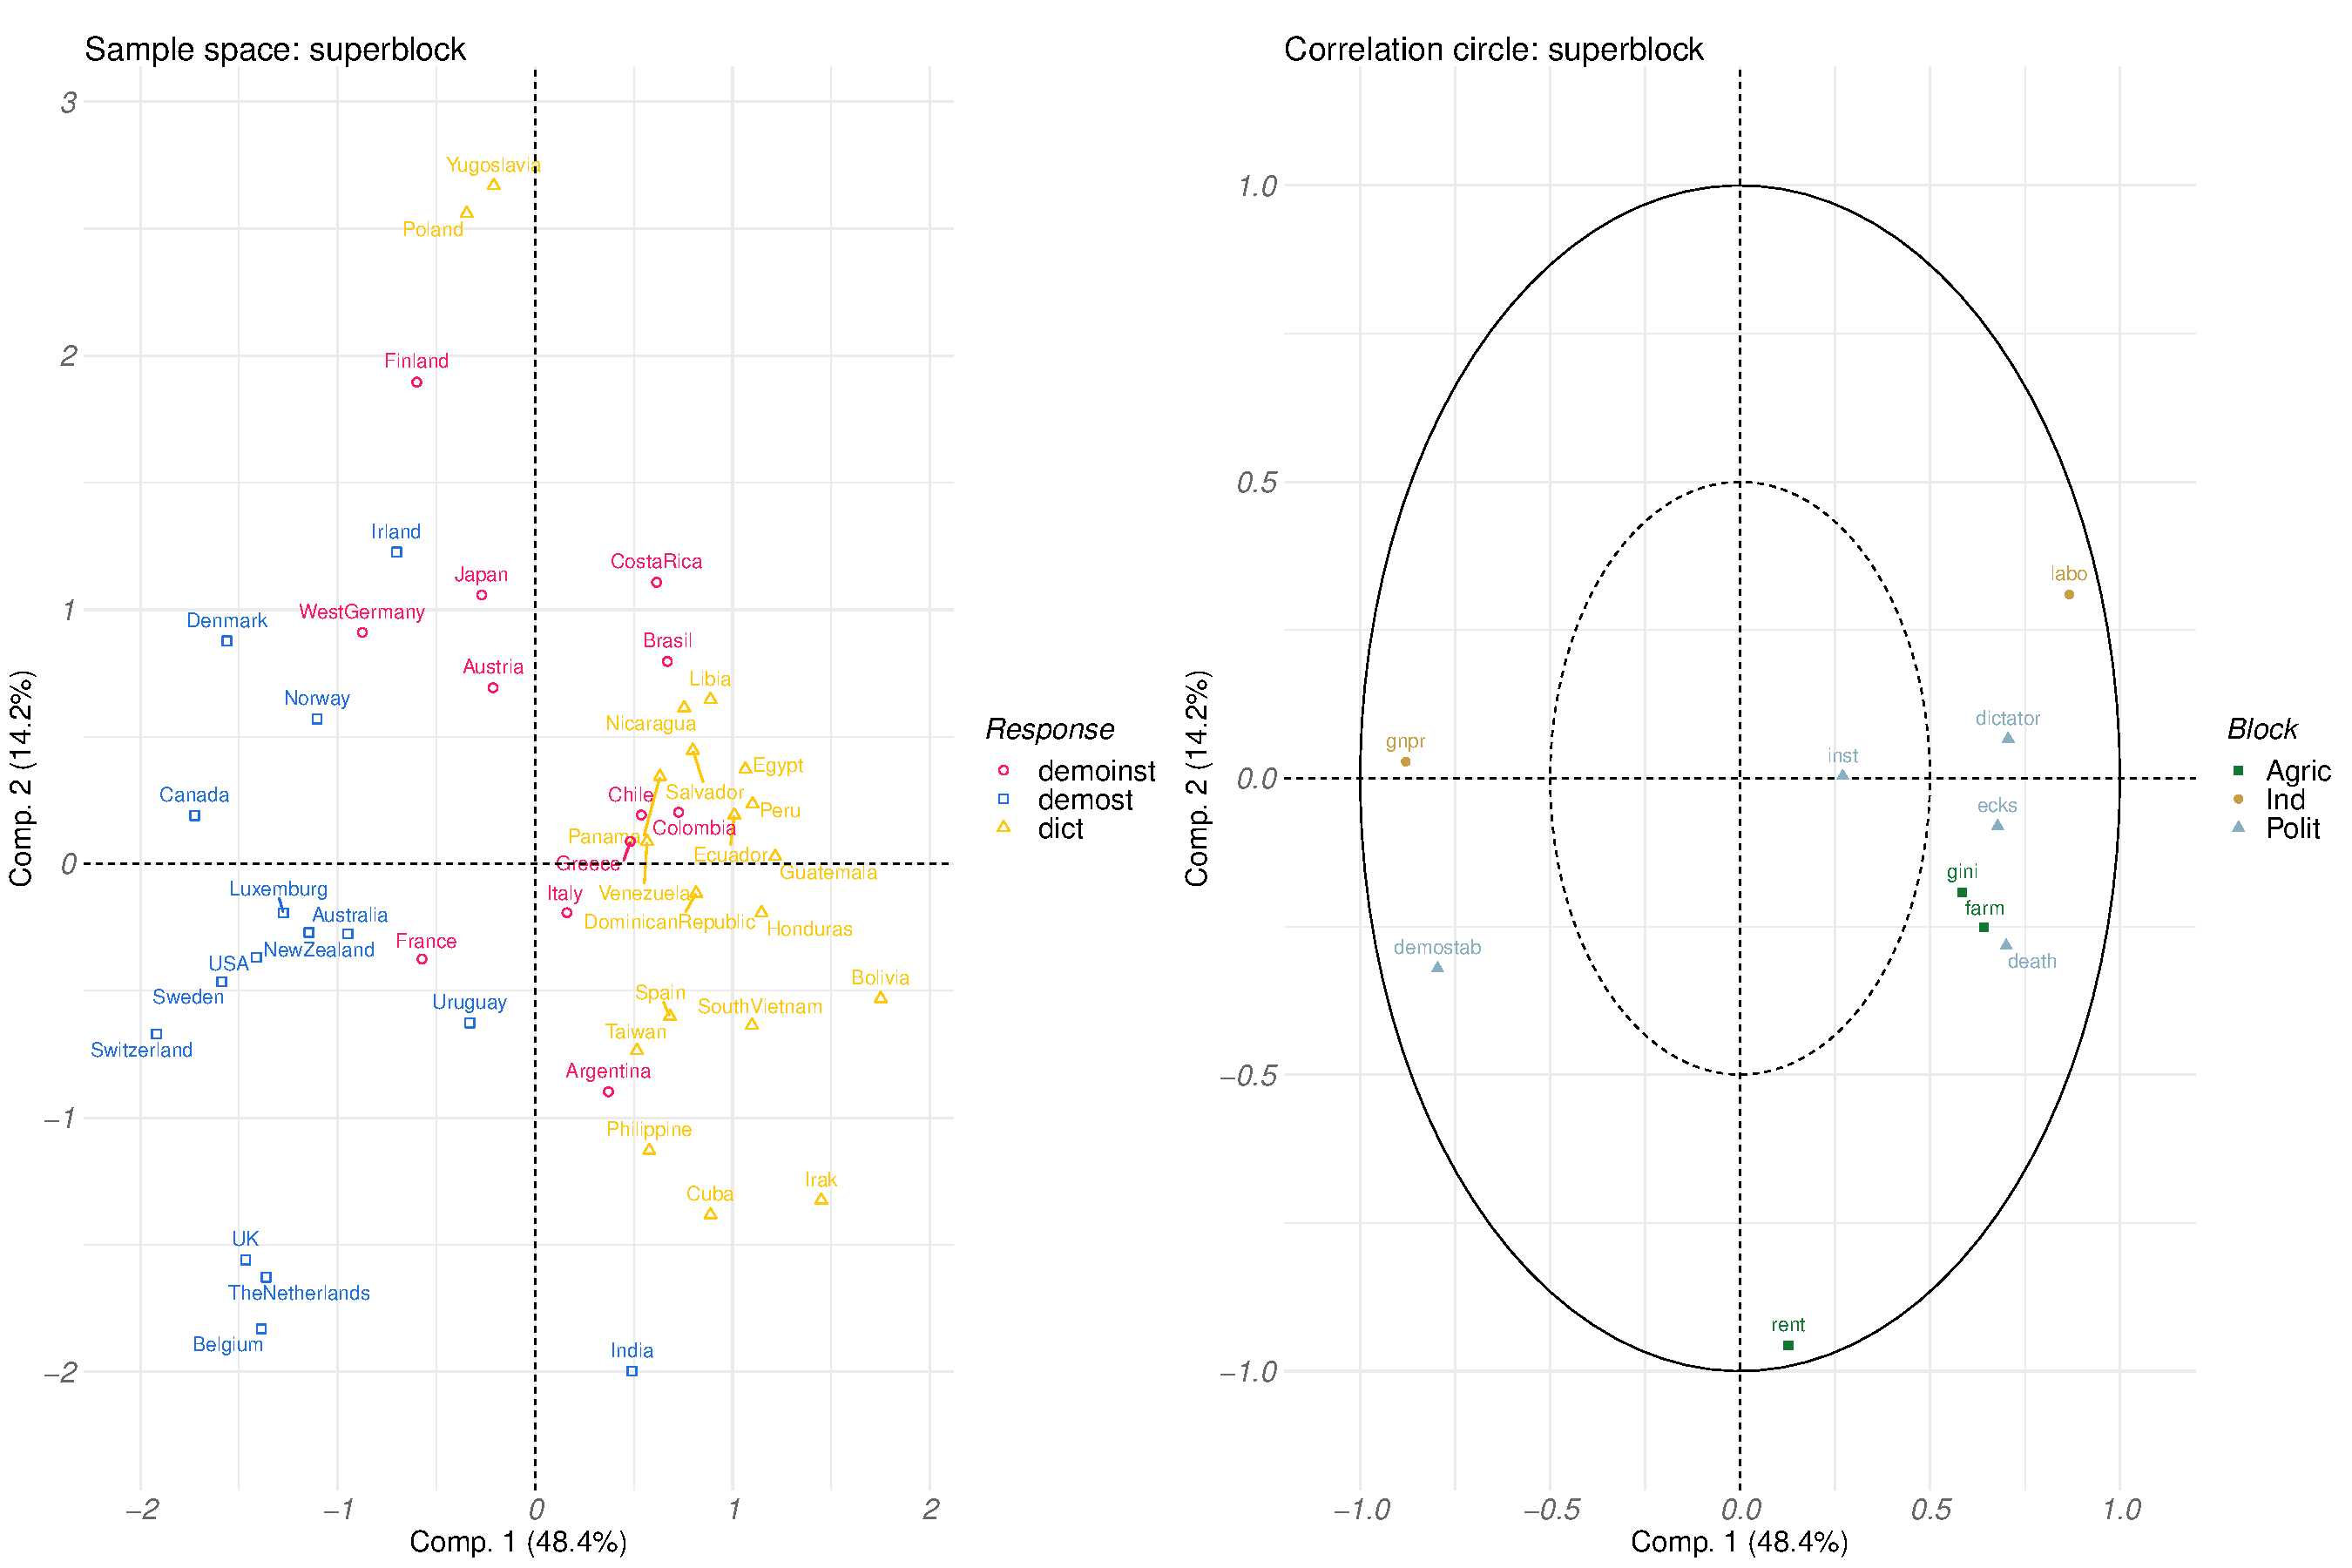
\includegraphics{RGCCA_files/figure-latex/unnamed-chunk-16-1} 

}

\caption[sample space and correlation cirle]{sample space and correlation cirle}\label{fig:unnamed-chunk-16}
\end{figure}
\end{CodeChunk}

\normalsize

The block-weight vectors solution of MCOA are displayed below:

\footnotesize

\begin{CodeChunk}
\begin{CodeInput}
R> plot(fit.mcoa, type = "weight",
+      block = 1:3, comp = 1,
+      display_order = FALSE, cex = 1.3)
\end{CodeInput}


\begin{center}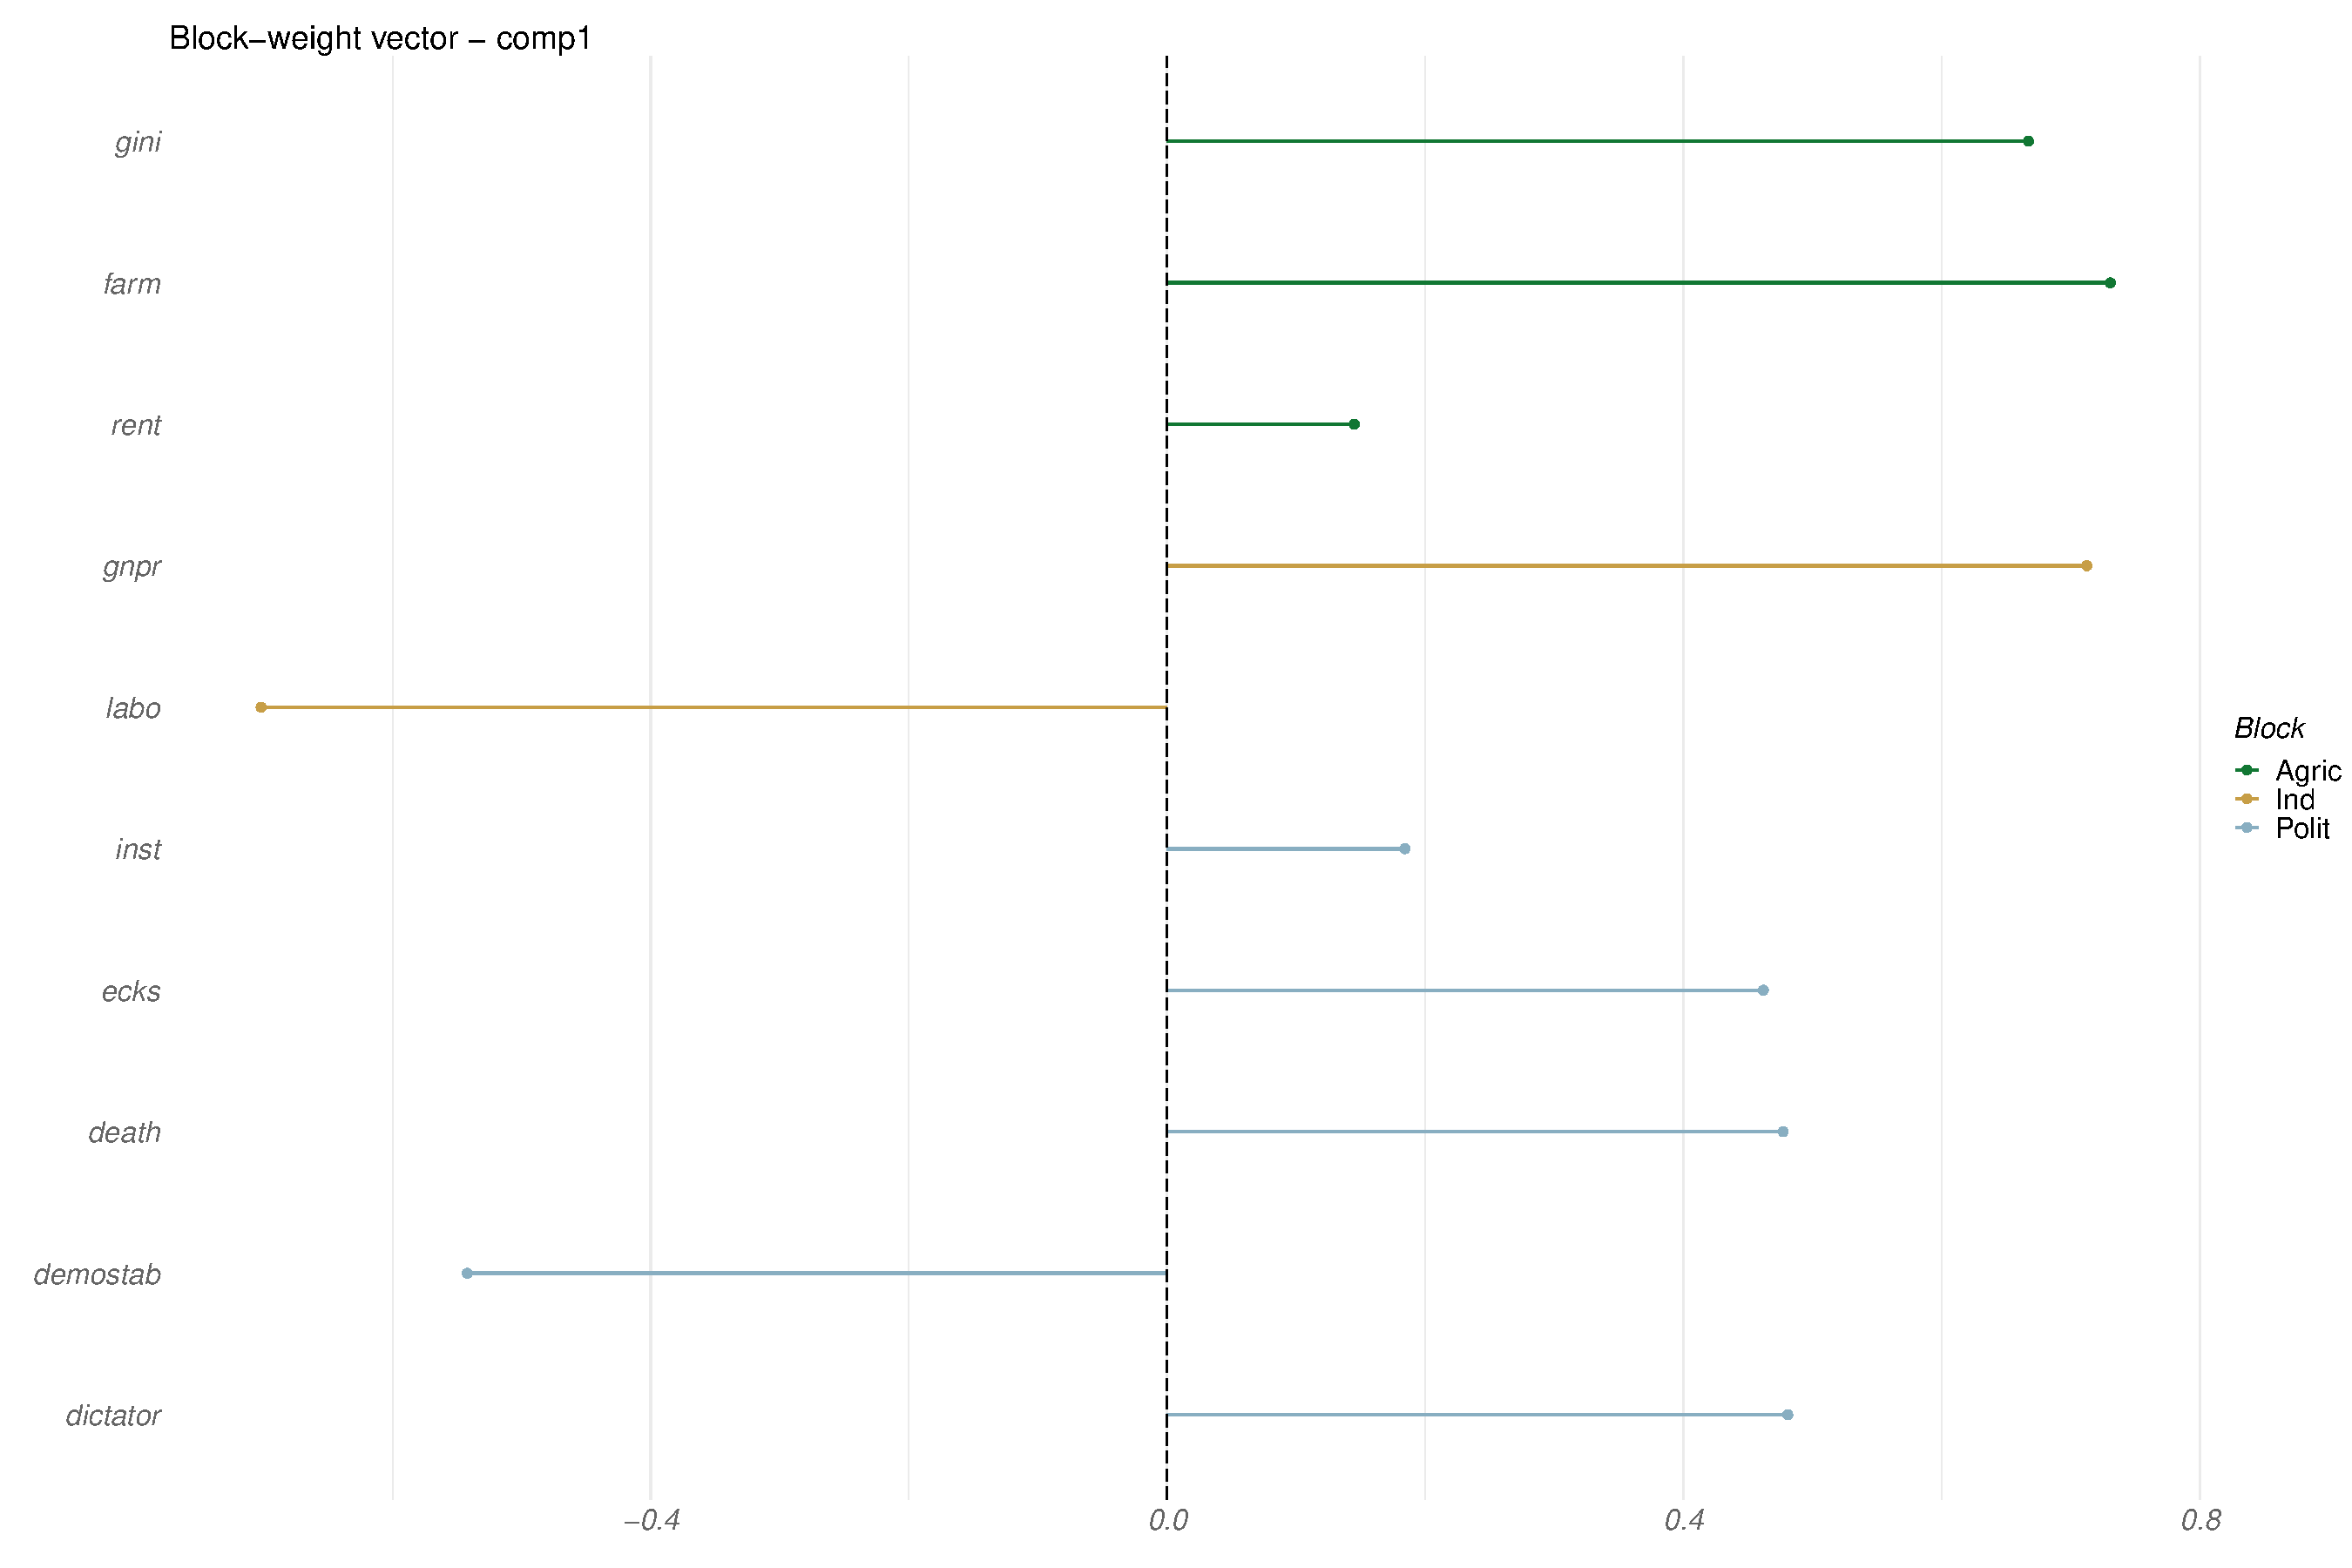
\includegraphics{RGCCA_files/figure-latex/unnamed-chunk-17-1} \end{center}

\end{CodeChunk}

\normalsize This model can be easily bootstrapped as follows:

\begin{CodeChunk}
\begin{CodeInput}
R> boot_out = rgcca_bootstrap(fit.mcoa, n_boot = 500)
\end{CodeInput}
\begin{CodeOutput}
Bootstrap samples sanity check...OK
\end{CodeOutput}
\end{CodeChunk}

The bootstrap confidence intervals are available using the
print()/plot() function

\footnotesize

\begin{CodeChunk}
\begin{CodeInput}
R> plot(boot_out, comp = 1,
+      display_order = FALSE, cex = 1.3)
\end{CodeInput}


\begin{center}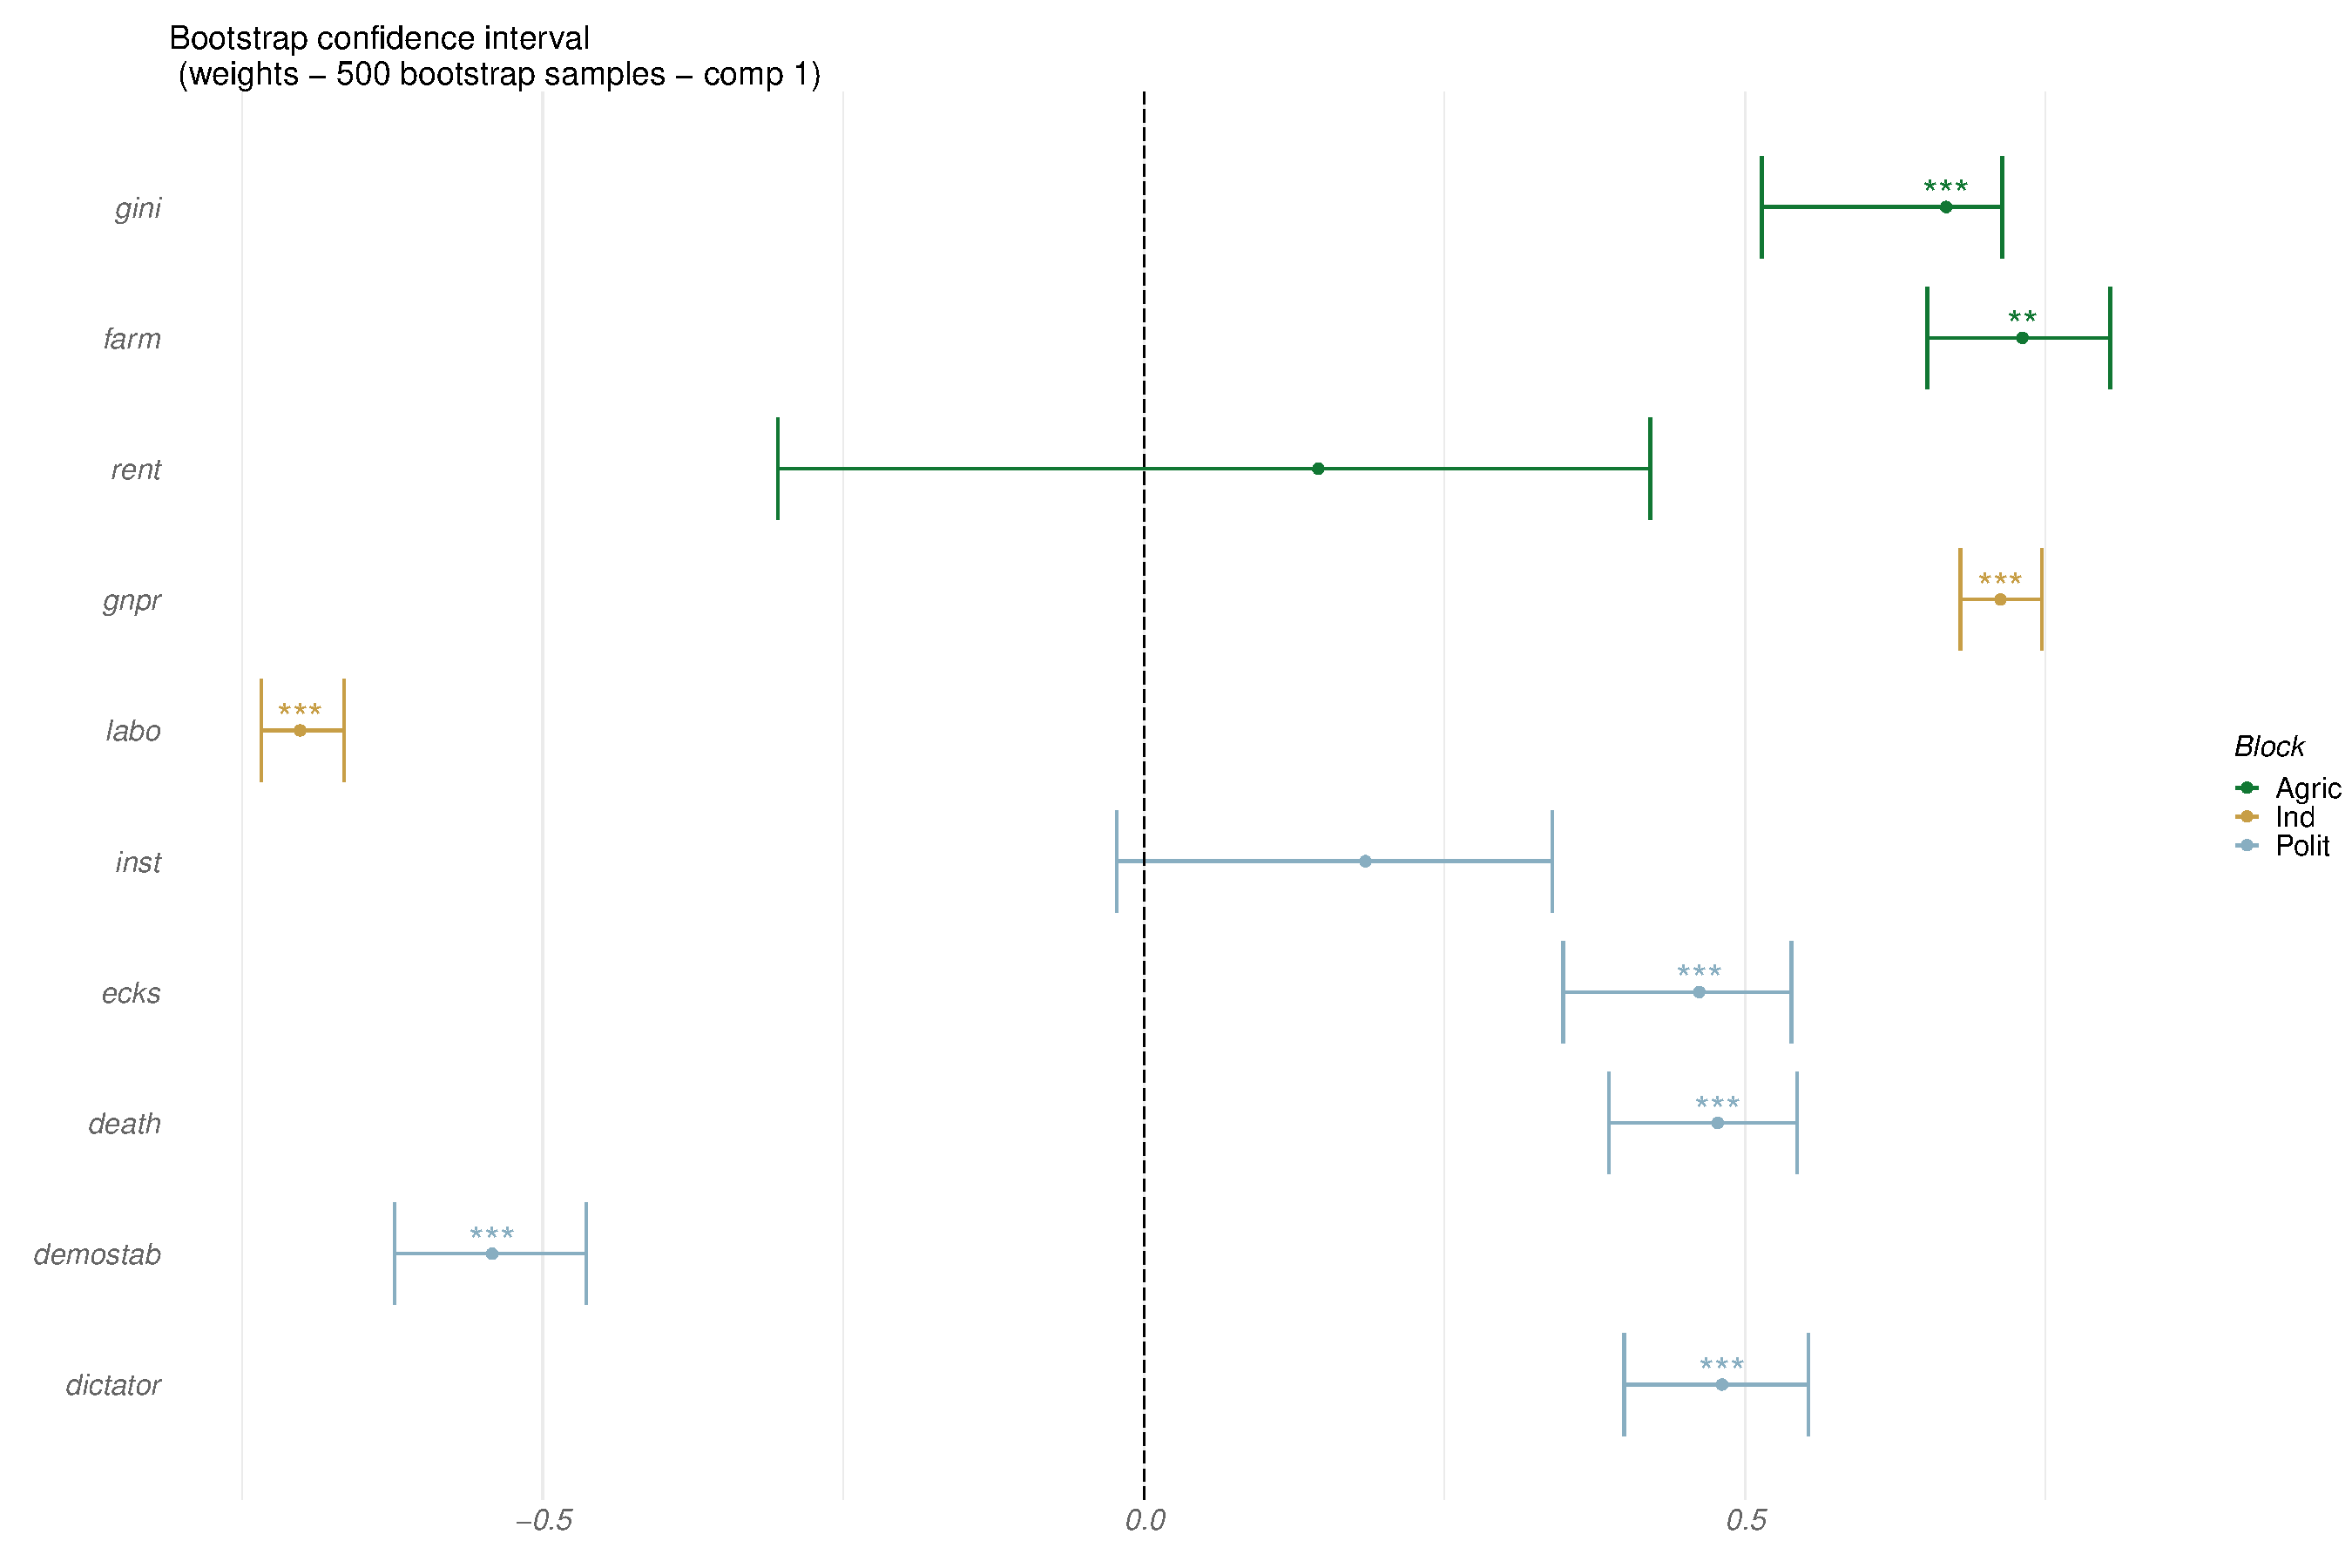
\includegraphics{RGCCA_files/figure-latex/unnamed-chunk-19-1} \end{center}

\end{CodeChunk}

\normalsize

\hypertarget{choice-of-the-shrinkage-parameter}{%
\subsection{Choice of the shrinkage
parameter}\label{choice-of-the-shrinkage-parameter}}

Three fully automatic strategies are proposed to select the optimal
shrinkage parameters:

\textbf{Choice of the shrinkage parameter using the Schafer and Strimmer
analytical formula \citep{Schafer2005}} For each block \(j\), an
``optimal'' shrinkage parameter \(\tau_j\) can be obtained from the
Schafer and Strimmer analytical formula \citep{Schafer2005} by setting
the \texttt{tau} argument of the the \texttt{rgcca()} function to
\texttt{"optimal"}.

\footnotesize

\begin{CodeChunk}
\begin{CodeInput}
R> fit = rgcca(blocks = A, connection=C, response=3,
+             tau = "optimal", scheme = "factorial")
\end{CodeInput}
\end{CodeChunk}

\normalsize

The optimal shrinkage parameters are given by:

\footnotesize

\begin{CodeChunk}
\begin{CodeInput}
R> fit$call$tau
\end{CodeInput}
\begin{CodeOutput}
[1] 0.08853216 0.02703256 0.08422566
\end{CodeOutput}
\end{CodeChunk}

\normalsize

This automatic estimation of the shrinkage parameters allows one to come
closer to the correlation criterion, even in the case of high
multicollinearity or when the number of individuals is smaller than the
number of variables.

As previously, all the fitted RGCCA object can be visualized/bootstraped
using the \texttt{print}, \texttt{plot()} and
\texttt{rgcca\_bootstrap()} functions.

\textbf{Choice of the shrinkage parameter by permutation strategy.} A
permutation based strategy very similar to the one proposed in
\citep{Witten2009a} has been also integrated within the RGCCA package
through the \texttt{rgcca\_permutation()} function. This function is
used to select automatically the regularization parameters for R/SGCCA.

For each set of regularization parameters (generally this will be a
\(J\)-dimensional vector), repeat the following \texttt{n\_perm} times,
for (\texttt{n\_perm} large):

\begin{enumerate}
\item [\label{p1}] The samples in $\mathbf X_1, \ldots, \mathbf X_J$ are
randomly permuted to obtained data sets $\mathbf X_1^*, \ldots, \mathbf X_J^*$.

\item [\label{p2}] S/RGCCA is run on the permuted data set
$\mathbf X_1^*, \ldots, \mathbf X_J^*$ to get block weight vectors
$\mathbf w_1^*, \ldots, \mathbf w_J^*$.

\item [\label{p3}]  Record $t^* = \displaystyle \sum_{j,k} c_{jk} g(\text{cov}(\mathbf X_j^*\mathbf w_j^*, \mathbf X_k^*\mathbf w_k^*))$.

\item [\label{p4}]  S/RGCCA is run on the original data
$\mathbf X_1, \ldots, \mathbf X_J$ to obtain the block weight vectors
$\mathbf w_1, \ldots, \mathbf w_J$.

\item [\label{p5}]  Record $t = \displaystyle \sum_{j,k} c_{jk} g(\text{cov}(\mathbf X_j\mathbf w_j, \mathbf X_k\mathbf w_k))$.

\item [\label{p6}]  The resulting p-value is given by the fraction of permuted
$t*$ that exceed the real $t$t obtained from the real data.
\end{enumerate}

Then choose the set of tuning parameters that gives the smallest value
in step (\ref{p6}).

This procedure is available though the \texttt{rgcca\_permutation()}
function.

\begin{CodeChunk}
\begin{CodeInput}
R> set.seed(123)
R> perm_out = rgcca_permutation(blocks = A, connection=C, 
+                              par_type = "tau",
+                              par_value = c(.51, .13, 0),
+                              par_length = 10,
+                              n_cores = 1,
+                              n_perms = 10)
\end{CodeInput}
\end{CodeChunk}

By default, the \texttt{rgcca\_permutation()} function takes 10 sets of
tuning parameters between min values (0 for RGCCA and \(1/sqrt(ncol)\)
for SGCCA) and 1. Results of the permutation procedure are
summarized/displayed using the generic \texttt{print()/plot()} function

\footnotesize

\begin{CodeChunk}
\begin{CodeInput}
R> print(perm_out)
\end{CodeInput}
\begin{CodeOutput}
Call: method='rgcca', superblock=FALSE, scale=TRUE, scale_block=TRUE, init='svd',
bias=TRUE, tol=1e-08, NA_method='nipals', ncomp=c(1,1,1), response=NULL,
comp_orth=TRUE 
There are J = 3 blocks.
The design matrix is:
      Agric Ind Polit
Agric     0   0     1
Ind       0   0     1
Polit     1   1     0

The factorial scheme is used.

Tuning parameters (tau) used: 
   Agric   Ind Polit
1  0.510 0.130     0
2  0.453 0.116     0
3  0.397 0.101     0
4  0.340 0.087     0
5  0.283 0.072     0
6  0.227 0.058     0
7  0.170 0.043     0
8  0.113 0.029     0
9  0.057 0.014     0
10 0.000 0.000     0

   Tuning parameters Criterion Permuted criterion    sd zstat p-value
1              Set 1      1.52              0.392 0.165  6.87       0
2              Set 2      1.54              0.400 0.168  6.76       0
3              Set 3      1.55              0.409 0.172  6.63       0
4              Set 4      1.57              0.420 0.176  6.50       0
5              Set 5      1.58              0.433 0.181  6.36       0
6              Set 6      1.61              0.448 0.187  6.20       0
7              Set 7      1.63              0.467 0.194  6.02       0
8              Set 8      1.67              0.493 0.203  5.82       0
9              Set 9      1.73              0.531 0.214  5.61       0
10            Set 10      1.93              0.665 0.230  5.52       0
The best combination is: Set 1 for a z score of 6.87 and a p-value of 0.
\end{CodeOutput}
\end{CodeChunk}

\normalsize

and displayed using the \texttt{plot()} function.

\footnotesize

\begin{CodeChunk}
\begin{CodeInput}
R> plot(perm_out, cex = 1.3)
\end{CodeInput}


\begin{center}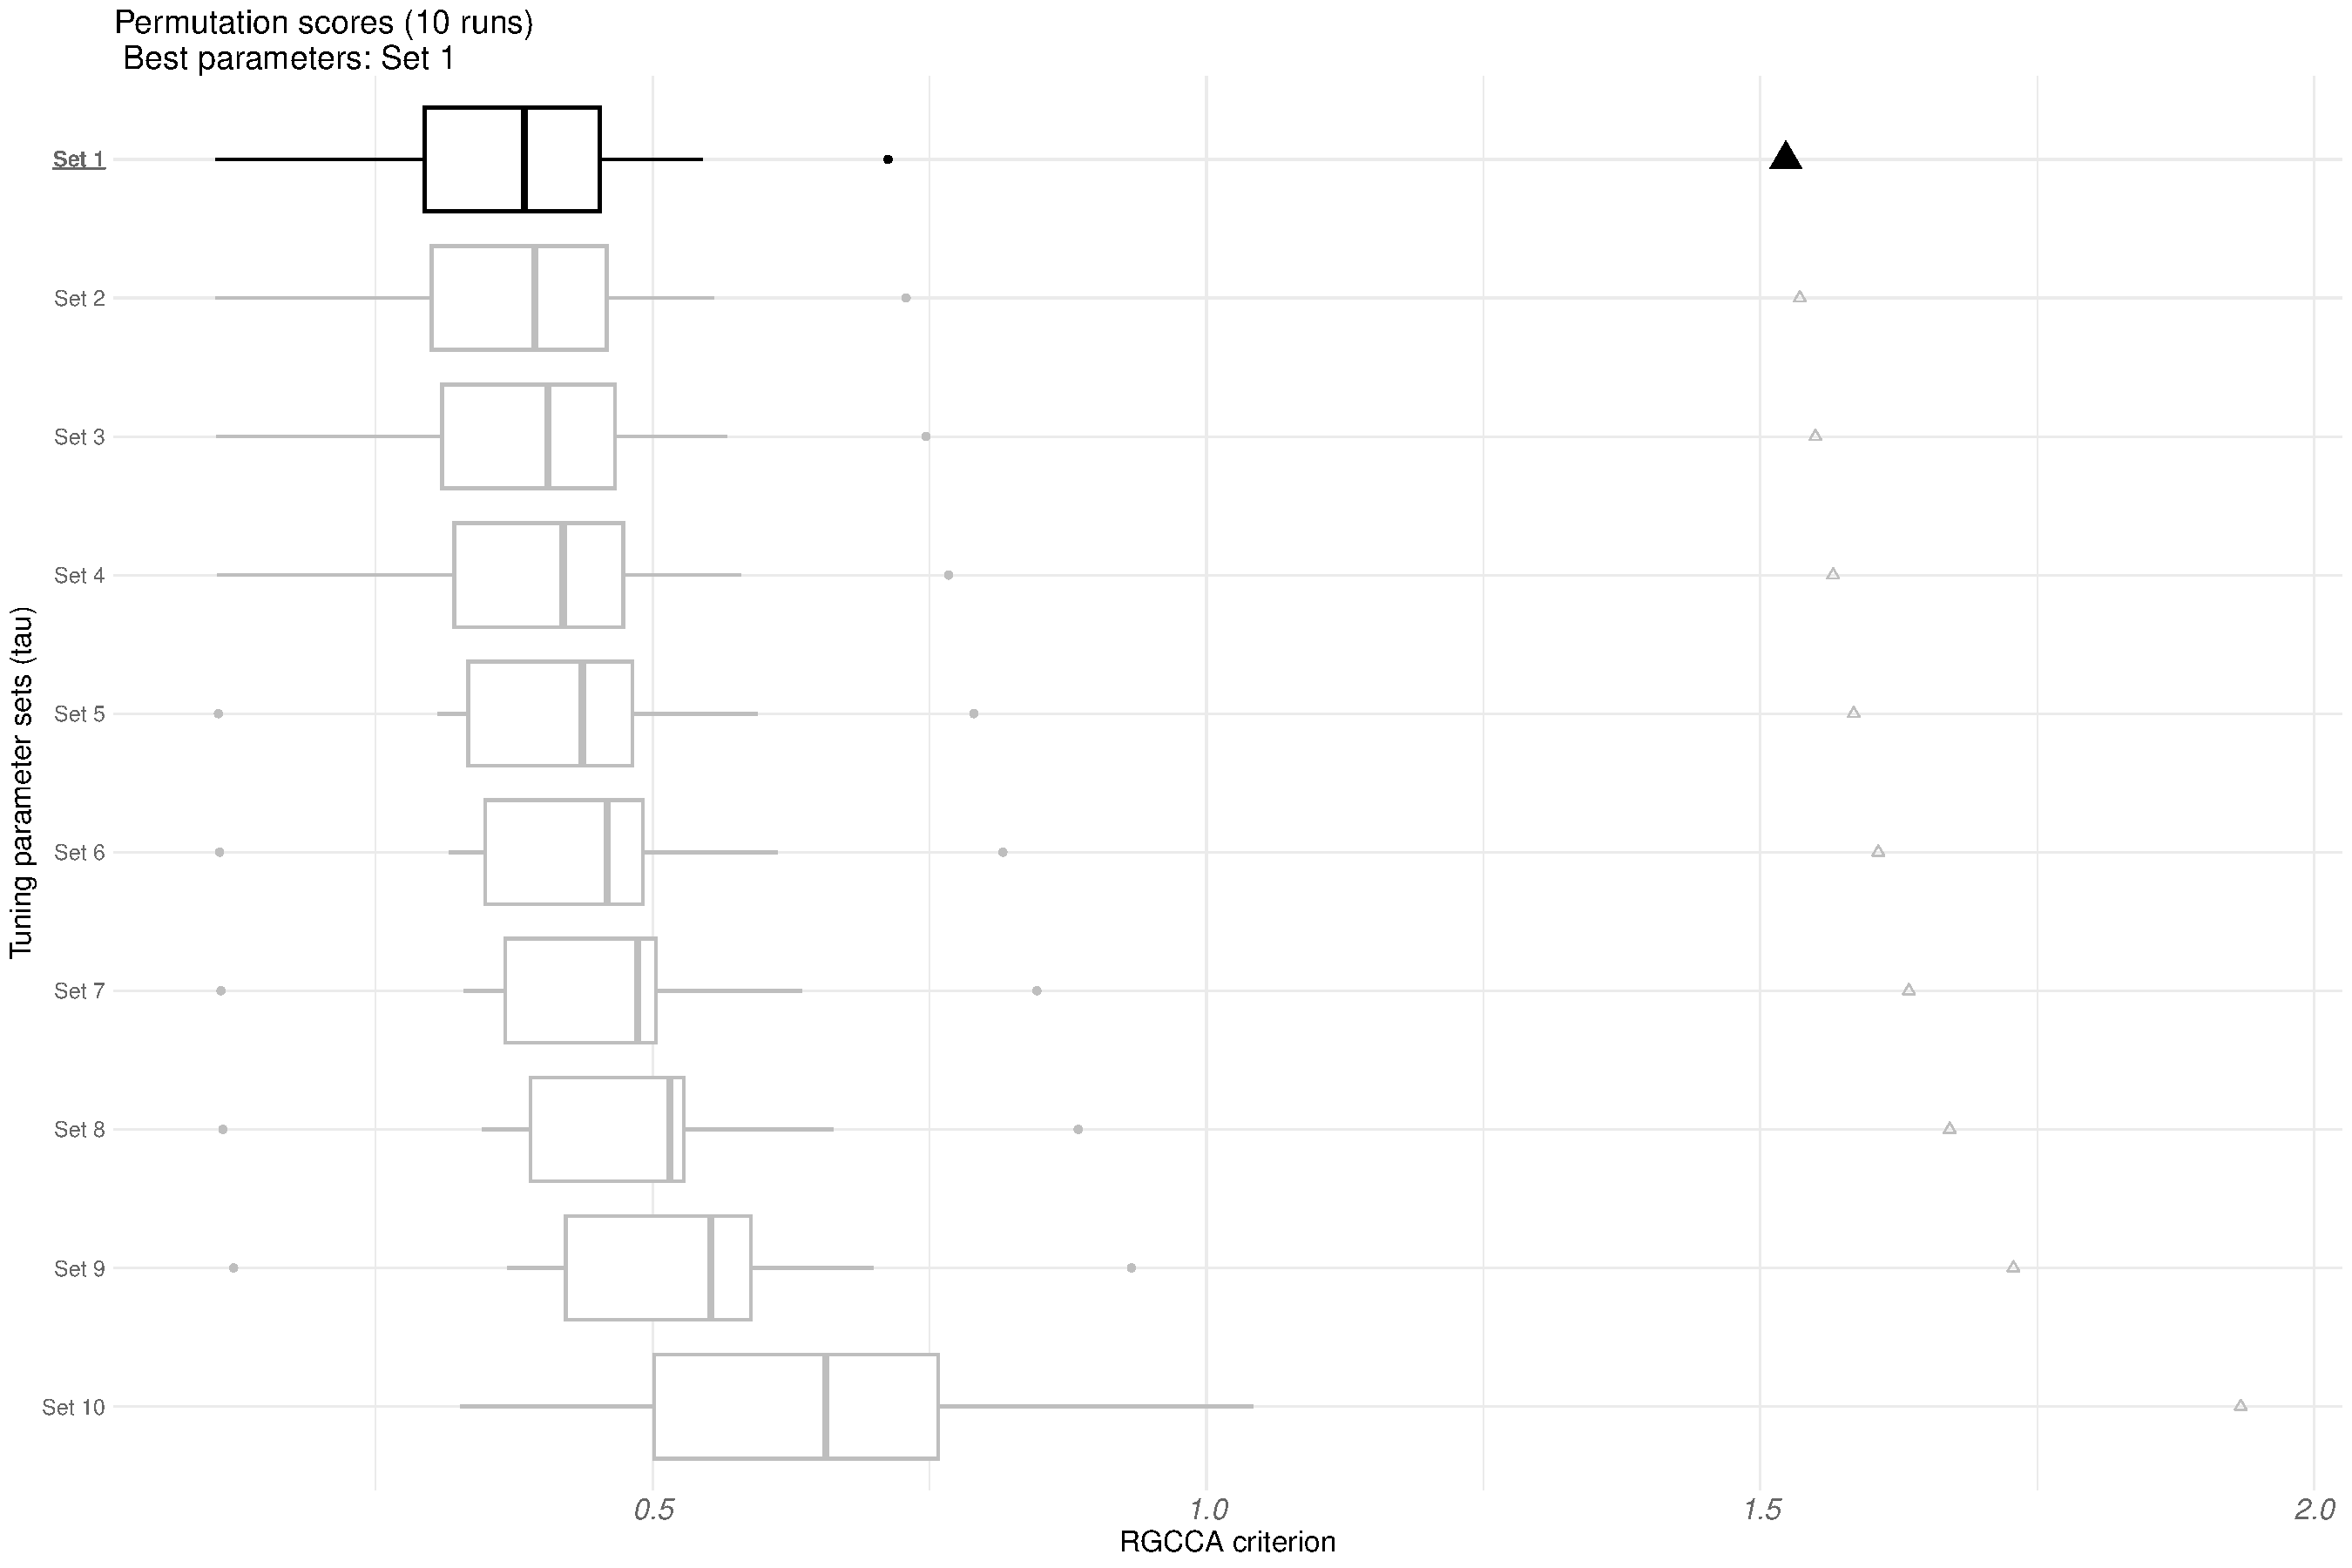
\includegraphics{RGCCA_files/figure-latex/unnamed-chunk-24-1} \end{center}

\end{CodeChunk}

\normalsize

The fitted permutation object, \texttt{perm\_out}, can be directly
provided as output of \texttt{rgcca()} and visualized/bootstrapped as
usual.

\footnotesize

\begin{CodeChunk}
\begin{CodeInput}
R> fit = rgcca(perm_out)
\end{CodeInput}
\end{CodeChunk}

\normalsize

Of course, it is possible to define explicitly the combination of
regularization parameters to be tested. In that case a matrix of
dimension \(K \times J\) is required. Each row of this matrix
corresponds to one set of tuning parameters.

\begin{CodeChunk}
\begin{CodeInput}
R> fit.perm = rgcca_permutation(A, connection = C,
+                              par_type = "tau",
+                              par_value = rbind(rep(1, 3),
+                                                seq(0, 1, l=3),
+                                                rep(0, 3),
+                                                sapply(A, RGCCA:::tau.estimate)),
+                              n_cores = 1, n_perms = 5)
\end{CodeInput}
\end{CodeChunk}

Alternatively a numeric vector of length \(J\) indicating the range of
values to be tested: from the minimum values (0 for RGCCA and
\(1/sqrt(ncol)\) for SGCCA) to the maximum values specified by the user
with \texttt{par\_value}.

\begin{CodeChunk}
\begin{CodeInput}
R> fit.perm = rgcca_permutation(A, connection = C,
+                              par_type = "tau",
+                              par_value = seq(0, 1, l=3),
+                              n_cores = 1, n_perms = 5)
\end{CodeInput}
\end{CodeChunk}

\textbf{Choice of the shrinkage parameter by cross-validation strategy.}
The optimal tuning parameters can also be determined by cross-validating
different indicators of quality, namely :

\begin{itemize}
\item
  For Classification: \texttt{Accuracy}, \texttt{Kappa}, \texttt{F1},
  \texttt{Sensitivity}, \texttt{Specificity}, \texttt{Pos\_Pred\_Value},
  \texttt{Neg\_Pred\_Value}, \texttt{Precision}, \texttt{Recall},
  \texttt{Detection\_Rate}, \texttt{Balanced\_Accuracy}.
\item
  For regression: \texttt{RMSE} and \texttt{MAE}.
\end{itemize}

This cross-validation protocol is made avalaible through the
\texttt{rgcca\_cv()} function. and is used for predicting the
qualitative variable political regime from Agriculture inequality and
Industrial development .

\begin{CodeChunk}
\begin{CodeInput}
R> blocks <- 
+   list(agriculture = Russett[, seq(3)],
+        industry = Russett[, 4:5],
+        lab = as.matrix(factor(apply(Russett[, 9:11], 1, which.max),
+                        labels = c("Stable", 
+                                   "Unstable",
+                                   "Dictator")))
+                )
R> 
R> set.seed(27) #my favorite number
R> inTraining <- caret:::createDataPartition(blocks[[3]], 
+                                   p = .75, list = FALSE)
R> training <- lapply(blocks, 
+                    function(x) x[inTraining, , drop = FALSE])
R> 
R> testing  <- lapply(blocks, 
+                    function(x) x[-inTraining, , drop = FALSE])
R> 
R> cv_out = rgcca_cv(blocks = training, response = 3, 
+                   par_type = "tau", 
+                   prediction_model = "rf", 
+                   n_run = 10, k = 3,
+                   validation = "kfold", 
+                   ncomp = 1, metric = "Accuracy")
\end{CodeInput}
\end{CodeChunk}

\texttt{rgcca\_cv()} relies on the \texttt{caret} package. As direct
consequence an astonishing large number of models are made available
(see \texttt{caret::modelLookup()}). Results of the cross validation
procedure are reported/displayed using the generic
\texttt{print()/plot()} function

\footnotesize

\begin{CodeChunk}
\begin{CodeInput}
R> print(cv_out)
\end{CodeInput}
\begin{CodeOutput}
Call: method='rgcca', superblock=FALSE, scale=TRUE, scale_block=TRUE, init='svd',
bias=TRUE, tol=1e-08, NA_method='nipals', ncomp=c(1,1,1), response=3,
comp_orth=TRUE 
There are J = 3 blocks.
The design matrix is:
            agriculture industry lab
agriculture           0        0   1
industry              0        0   1
lab                   1        1   0

The factorial scheme is used.

Tuning parameters (tau) used: 
   agriculture industry lab
1        1.000    1.000   0
2        0.889    0.889   0
3        0.778    0.778   0
4        0.667    0.667   0
5        0.556    0.556   0
6        0.444    0.444   0
7        0.333    0.333   0
8        0.222    0.222   0
9        0.111    0.111   0
10       0.000    0.000   0

Validation: kfold with 3 folds and 10 run(s)) 
Prediction model: rf 

   Tuning parameters Mean Accuracy     Sd
1     1.00/1.00/0.00         0.683 0.1226
2     0.89/0.89/0.00         0.689 0.1136
3     0.78/0.78/0.00         0.683 0.1036
4     0.67/0.67/0.00         0.669 0.1014
5     0.56/0.56/0.00         0.681 0.0981
6     0.44/0.44/0.00         0.686 0.0946
7     0.33/0.33/0.00         0.675 0.0963
8     0.22/0.22/0.00         0.678 0.1132
9     0.11/0.11/0.00         0.683 0.0939
10    0.00/0.00/0.00         0.642 0.0982

The best combination is: 0.89/0.89/0.00 for a mean Accuracy of 0.689.
\end{CodeOutput}
\end{CodeChunk}

\normalsize

and displayed using the \texttt{plot()} function.

\footnotesize

\begin{CodeChunk}
\begin{CodeInput}
R> plot(cv_out, cex = 1.3)
\end{CodeInput}


\begin{center}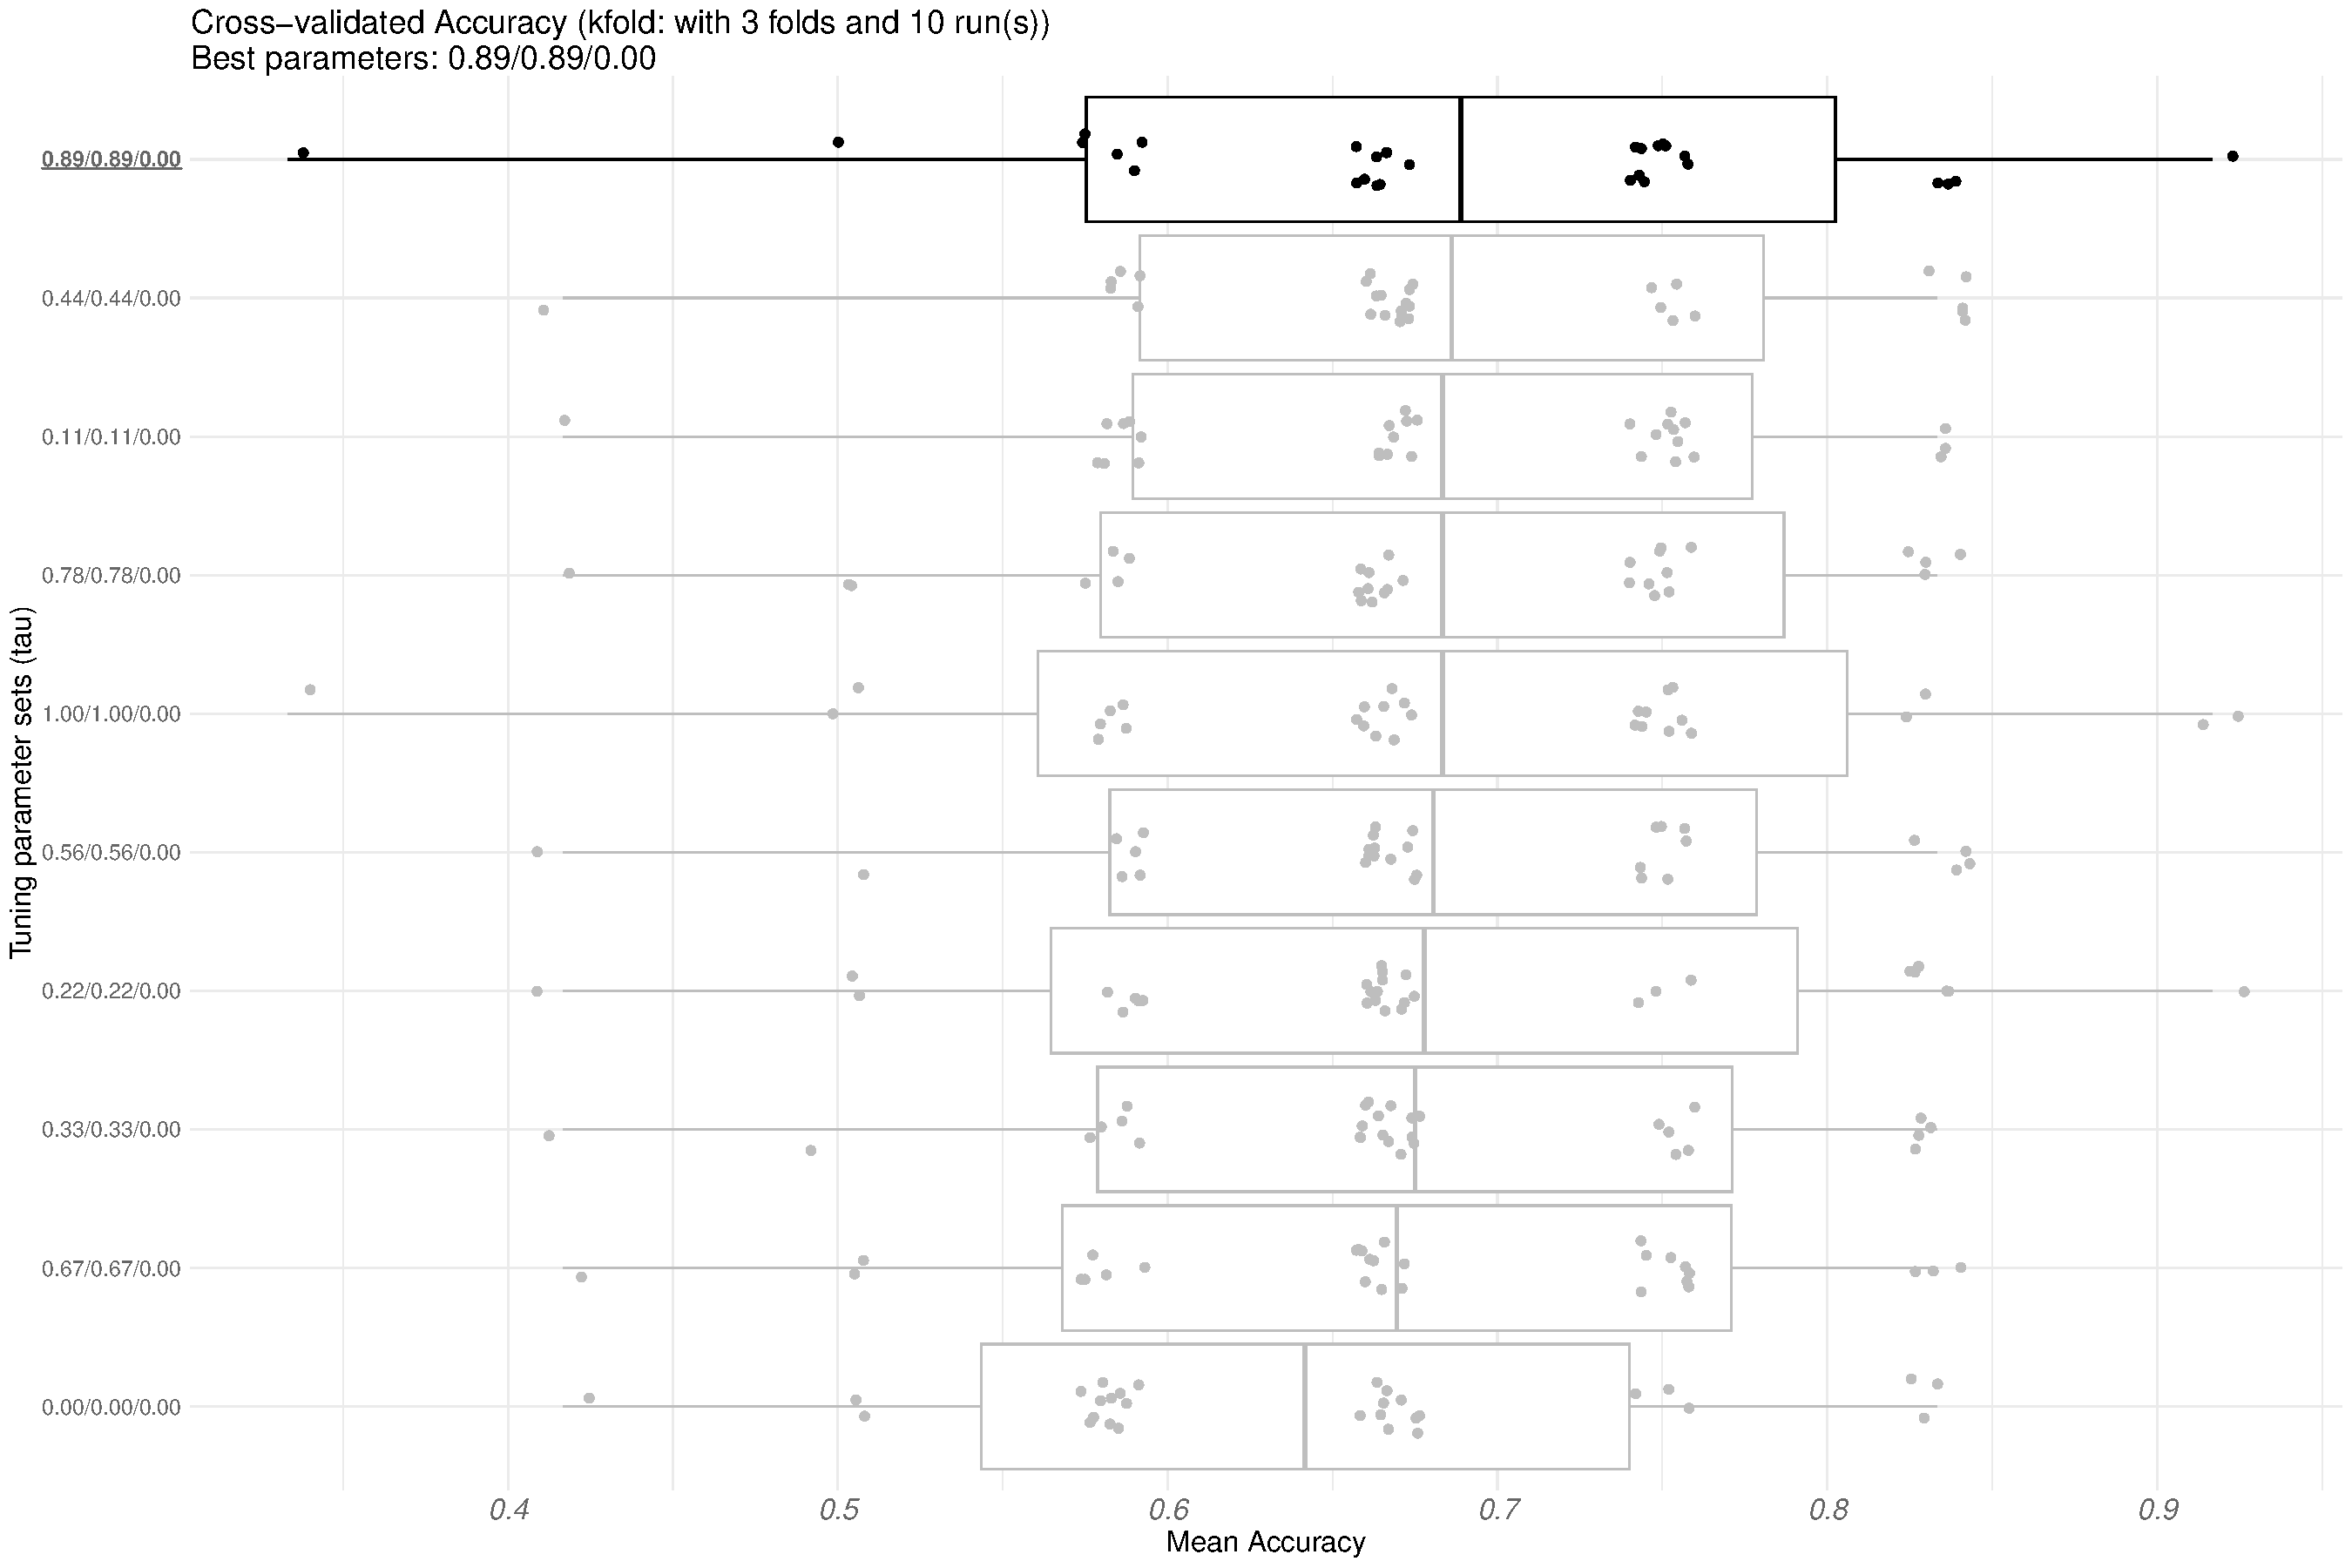
\includegraphics{RGCCA_files/figure-latex/unnamed-chunk-30-1} \end{center}

\end{CodeChunk}

\normalsize

Of course, the fitted cval object can be provided as output of
\texttt{rgcca()} and resulting optimal model can be
visualized/bootstrapped as usual.

\footnotesize

\begin{CodeChunk}
\begin{CodeInput}
R> fit = rgcca(cv_out)
\end{CodeInput}
\end{CodeChunk}

\normalsize

At last, \texttt{rgcca\_predict()} can be used for predicting new
blocks.

\footnotesize

\begin{CodeChunk}
\begin{CodeInput}
R> perf = rgcca_predict(fit, blocks_test = testing, prediction_model = "lda")
\end{CodeInput}
\end{CodeChunk}

\normalsize

and a \texttt{caret} summary of the performances be reported

\footnotesize

\begin{CodeChunk}
\begin{CodeInput}
R> perf$results$lab$confusion$test
\end{CodeInput}
\begin{CodeOutput}
Confusion Matrix and Statistics

          Reference
Prediction Dictator Stable Unstable
  Dictator        5      0        2
  Stable          0      3        1
  Unstable        0      0        0

Overall Statistics
                                          
               Accuracy : 0.7273          
                 95% CI : (0.3903, 0.9398)
    No Information Rate : 0.4545          
    P-Value [Acc > NIR] : 0.06478         
                                          
                  Kappa : 0.5541          
                                          
 Mcnemar's Test P-Value : NA              

Statistics by Class:

                     Class: Dictator Class: Stable Class: Unstable
Sensitivity                   1.0000        1.0000          0.0000
Specificity                   0.6667        0.8750          1.0000
Pos Pred Value                0.7143        0.7500             NaN
Neg Pred Value                1.0000        1.0000          0.7273
Prevalence                    0.4545        0.2727          0.2727
Detection Rate                0.4545        0.2727          0.0000
Detection Prevalence          0.6364        0.3636          0.0000
Balanced Accuracy             0.8333        0.9375          0.5000
\end{CodeOutput}
\end{CodeChunk}

\normalsize

All the functions presented previously has been adapted to sparse
analysis. This will be illustrated in the next section.

\hypertarget{high-dimensional-case-study-glioma-data}{%
\section{High dimensional case study: Glioma
Data}\label{high-dimensional-case-study-glioma-data}}

\textbf{Biological problem.} Brain tumors are the most common solid
tumors in children and have the highest mortality rate of all pediatric
cancers. Despite advances in multimodality therapy, children with pHGG
invariably have an overall survival of around 20\% at 5 years. Depending
on their location (e.g.~brainstem, central nuclei, or supratentorial),
pHGG present different characteristics in terms of radiological
appearance, histology, and prognosis. Our hypothesis is that pHGG have
different genetic origins and oncogenic pathways depending on their
location. Thus, the biological processes involved in the development of
the tumor may be different from one location to another, as it has been
frequently suggested.

\textbf{Description of the data.} Pretreatment frozen tumor samples were
obtained from 53 children with newly diagnosed pHGG from Necker Enfants
Malades (Paris, France) \citep{Puget2012}. The 53 tumors are divided
into 3 locations: supratentorial (HEMI), central nuclei (MIDL), and
brain stem (DIPG). The final dataset is organized in 3 blocks of
variables defined for the 53 tumors: the first block
\(\ensuremath{\mathbf{X}}_1\) provides the expression of \(15702\) genes
(GE). The second block \(\ensuremath{\mathbf{X}}_2\) contains the
imbalances of \(1229\) segments (CGH) of chromosomes.
\(\ensuremath{\mathbf{X}}_3\) is a block of dummy variables describing
the categorical variable location. One dummy variable has been left out
because of redundancy with he others.

\footnotesize

\begin{CodeChunk}
\begin{CodeInput}
R> # Download the dataset's package at http://biodev.cea.fr/sgcca/.
R> # --> gliomaData_0.4.tar.gz
R> 
R> require(gliomaData)
\end{CodeInput}
\begin{CodeOutput}
Loading required package: gliomaData
\end{CodeOutput}
\begin{CodeInput}
R> data(ge_cgh_locIGR)
R> 
R> blocks <- ge_cgh_locIGR$multiblocks
R> Loc <- factor(ge_cgh_locIGR$y)
R> levels(Loc) <- colnames(ge_cgh_locIGR$multiblocks$y)
R> blocks[[3]] = Loc
R> 
R> # check dimensions of the blocks
R> sapply(blocks, NCOL)
\end{CodeInput}
\begin{CodeOutput}
   GE   CGH     y 
15702  1229     1 
\end{CodeOutput}
\end{CodeChunk}

\normalsize

We impose \(\mathbf{X}_1\) and \(\mathbf{X}_2\) to be connected to
\(\mathbf{X}_3\). This design is commonly used in many applications and
is oriented toward the prediction of the location. The argument
\texttt{response=3} of the \texttt{rgcca()} function encodes this
design.

\footnotesize

\begin{CodeChunk}
\begin{CodeInput}
R> fit.rgcca = rgcca(blocks = blocks, response = 3, ncomp = 1)
\end{CodeInput}
\end{CodeChunk}

\normalsize

when the response variable is qualitative, two steps are implicitly
performed: (i) disjunctive coding and (ii) the associated shrinkage
parameter is set to \(0\) regardless of the value specified by the user.

\footnotesize

\begin{CodeChunk}
\begin{CodeInput}
R> fit.rgcca$call$connection
\end{CodeInput}
\begin{CodeOutput}
    GE CGH y
GE   0   0 1
CGH  0   0 1
y    1   1 0
\end{CodeOutput}
\end{CodeChunk}

\normalsize

\footnotesize

\begin{CodeChunk}
\begin{CodeInput}
R> fit.rgcca$call$tau
\end{CodeInput}
\begin{CodeOutput}
[1] 1 1 0
\end{CodeOutput}
\end{CodeChunk}

\normalsize

At last, from the dimension of each block (\(n>p\) or \(n\leq p\)),
\texttt{rgcca()} selects automatically the dual formulation for
\(\mathbf{X}_1\) and \(\mathbf{X}_2\) and the primal one for
\(\mathbf{X}_3\). The formulation used for each block is returned using
the following command:

\footnotesize

\begin{CodeChunk}
\begin{CodeInput}
R> fit.rgcca$primal_dual
\end{CodeInput}
\begin{CodeOutput}
[1] "dual"   "dual"   "primal"
\end{CodeOutput}
\end{CodeChunk}

\normalsize

The dual formulation make the RGCCA algorithm highly efficient even in a
high dimensional setting.

\footnotesize

\begin{CodeChunk}
\begin{CodeInput}
R> system.time(
+   rgcca(blocks = blocks, response = 3)
+ )
\end{CodeInput}
\begin{CodeOutput}
   user  system elapsed 
   3.13    0.06    3.39 
\end{CodeOutput}
\end{CodeChunk}

\normalsize

RGCCA enables visual inspection of the spatial relationships between
classes. This facilitates assessment of the quality of the
classification and makes it possible to readily determine which
components capture the discriminant information.

\footnotesize

\begin{CodeChunk}
\begin{CodeInput}
R> plot(fit.rgcca, type = "sample", block=1:2,
+      comp = 1, response = Loc)
\end{CodeInput}


\begin{center}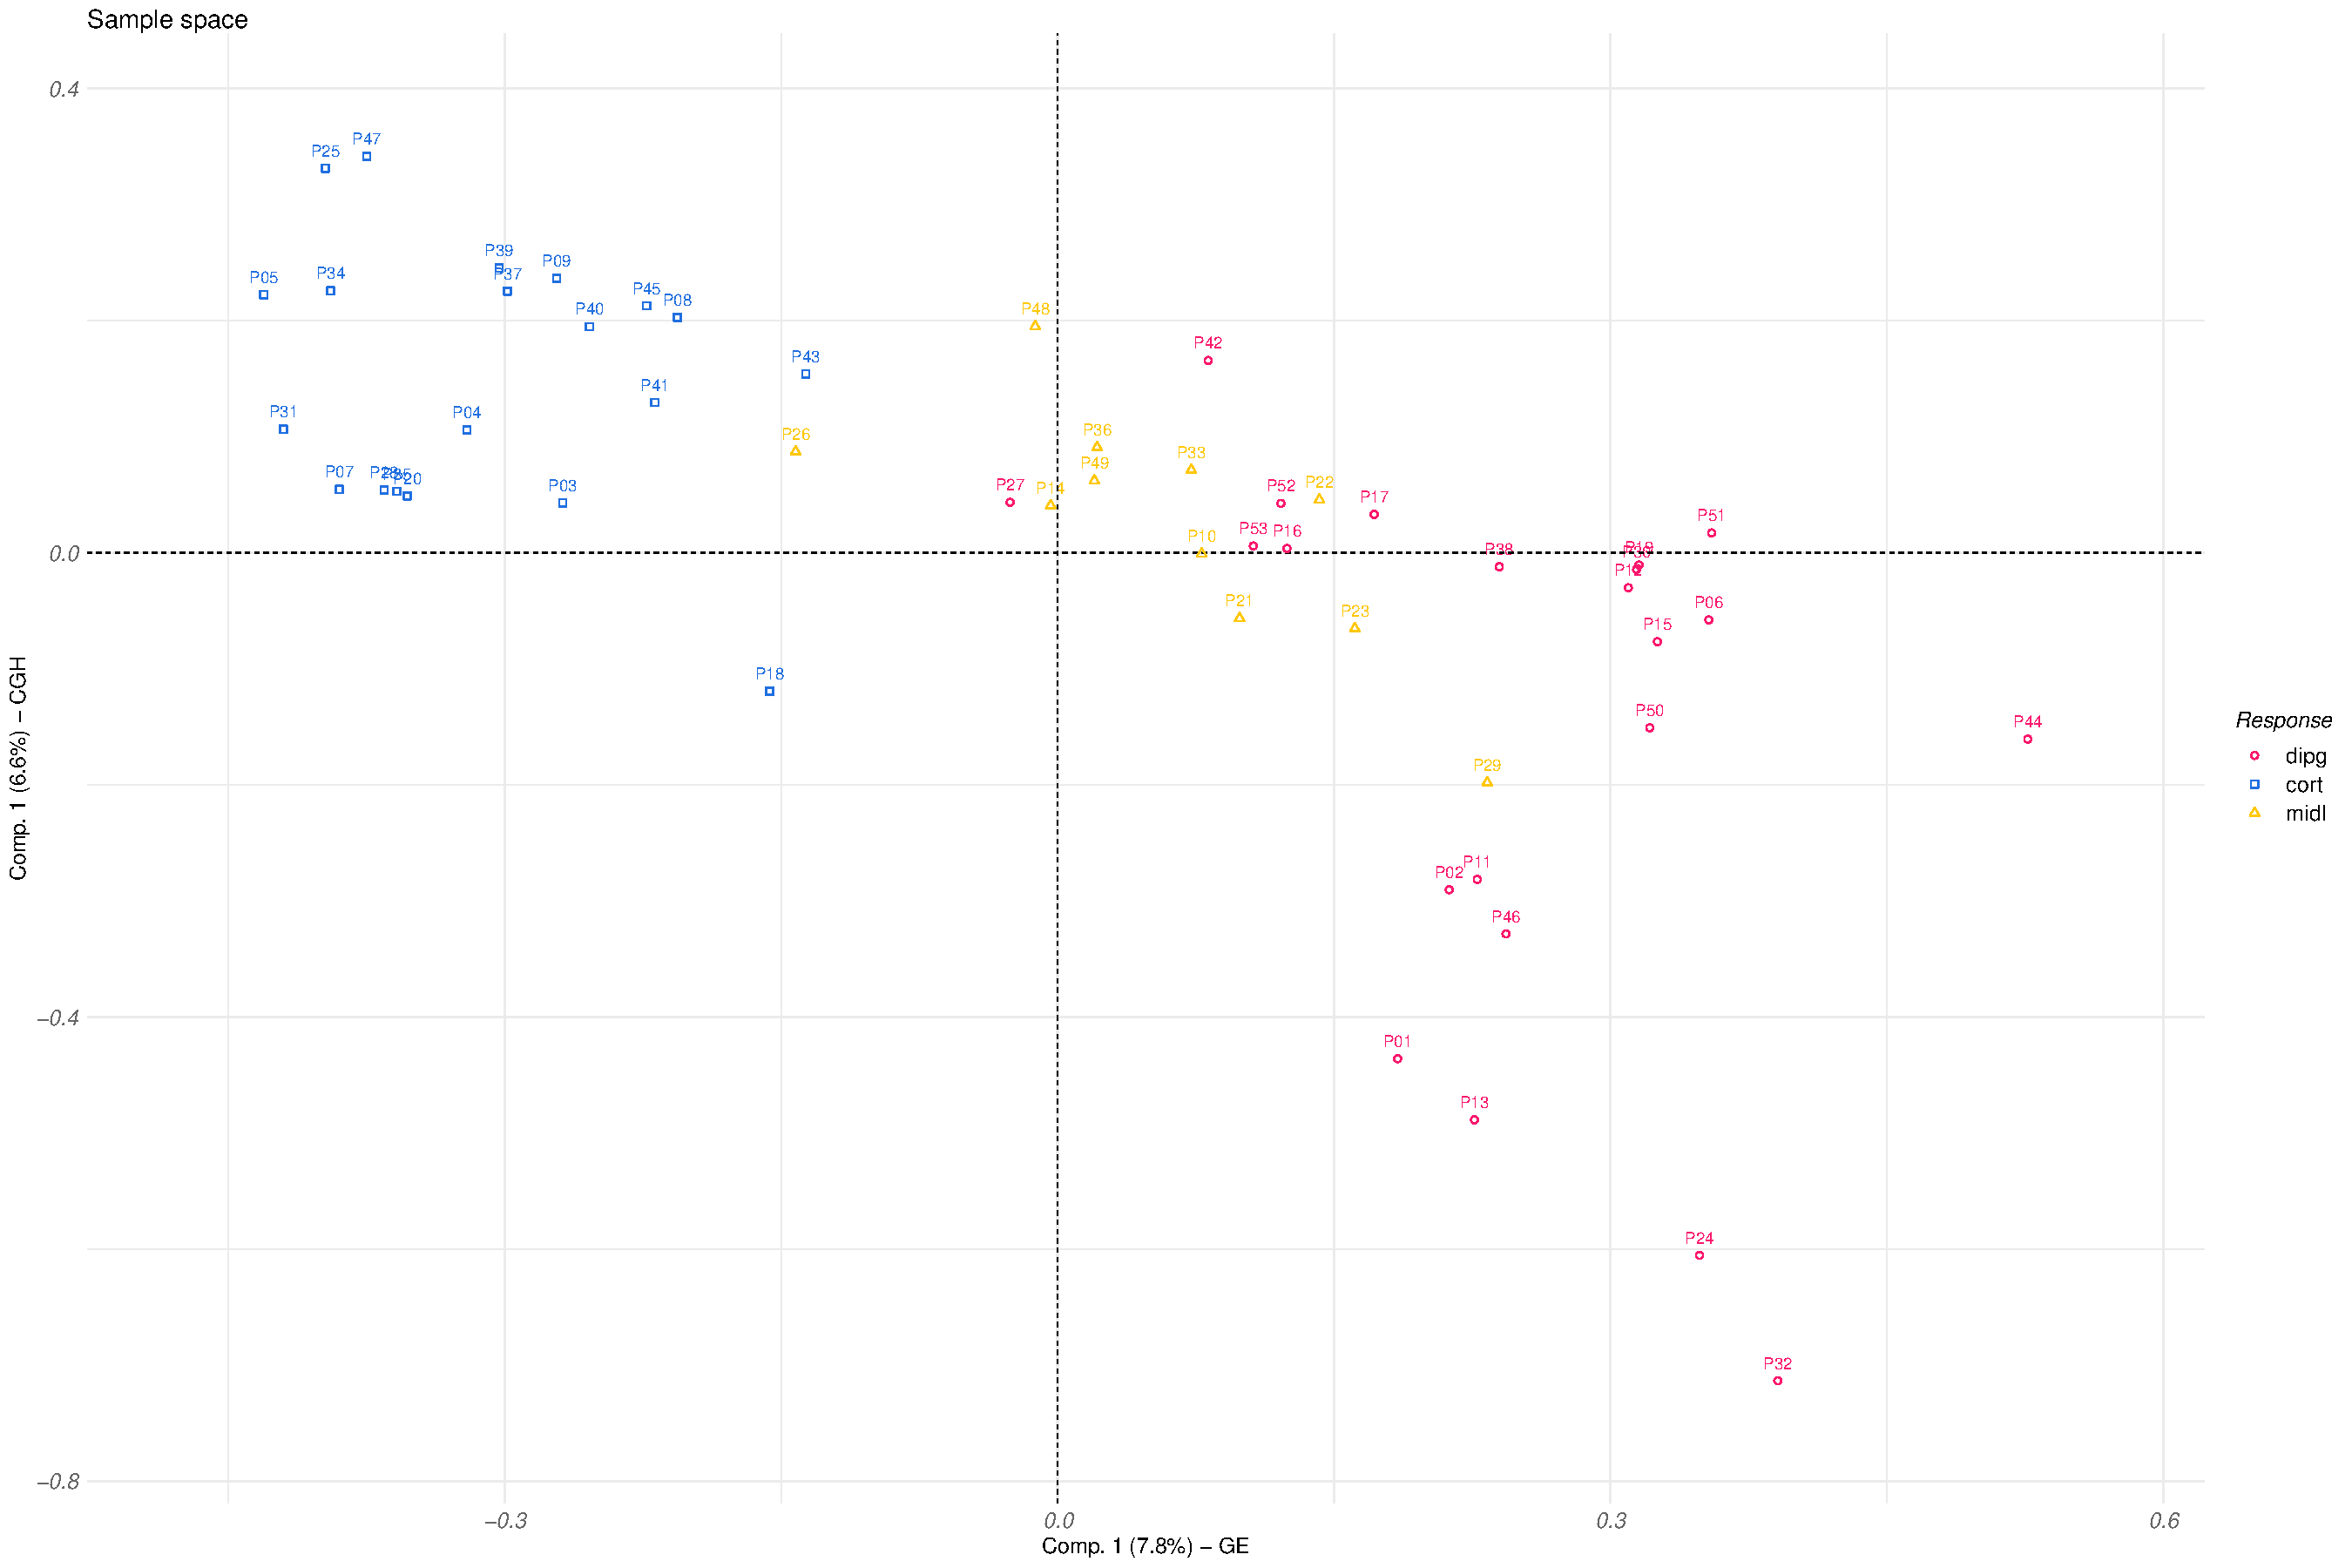
\includegraphics{RGCCA_files/figure-latex/unnamed-chunk-40-1} \end{center}

\end{CodeChunk}

\normalsize

For easier interpretation of the results, especially in high-dimensional
settings, it is often appropriate to add, within the RGCCA optimization
problem, penalties promoting sparsity. For that purpose, an \(\ell_1\)
penalization on the weight vectors
\(\mathbf{a}_1, \ldots, \mathbf{a}_J\) is applied. the \texttt{sparsity}
argument of \texttt{rgcca()} varies between 1/sqrt(ncol) and 1 (larger
values of \texttt{sparsity} correspond to less penalization) and control
the amount of sparsity of the weight vectors
\(\mathbf{a}_1, \ldots, \mathbf{a}_J\). If \texttt{sparsity} is a
vector, \(\ell_1\)-penalties are the same for all the weights
corresponding to the same block but different components:

\begin{equation}
\forall h, \Vert \ensuremath{\mathbf{a}}_j^{(h)} \Vert_{\ell_1} \leq c_{1j} \sqrt{p_j},
\end{equation}

with \(p_j\) the number of variables of \(\ensuremath{\mathbf{X}}_j\).

If \texttt{sparsity} is a matrix, row \(h\) of \texttt{sparsity} defines
the constraints applied to the weights corresponding to components
\(h\):

\begin{equation}
\forall h, \Vert \ensuremath{\mathbf{a}}_j^{(h)} \Vert_{\ell_1} \leq c_1[h,j] \sqrt{p_j}.
\end{equation}

\hypertarget{sgcca-for-the-glioma-dataset}{%
\subsection{SGCCA for the Glioma
dataset}\label{sgcca-for-the-glioma-dataset}}

In this situation, the optimal sparsity parameters is usually chosen to
minimizing the cross-validated error rate. We decide to upper bound the
sparsity paamerters for X1 and X3 to .2, to achieved an attactive amount
of sparsity.

\begin{CodeChunk}
\begin{CodeInput}
R> set.seed(27) #my favorite number
R> cv_out <- rgcca_cv(blocks, response = 3, 
+                    par_type = "sparsity",
+                    par_value = c(.2, .2, 0), 
+                    par_length = 10, 
+                    prediction_model = "lda",
+                    validation = "kfold",
+                    k = 3, n_run = 10, metric = "Accuracy",
+                    n_cores = 15)
\end{CodeInput}
\end{CodeChunk}

As usual, we can report the results of this cross-validation using the
generic \texttt{print()} and \texttt{plot()} functions and build the
optimal model using the fitted \texttt{cval} object as argument of
\texttt{rgcca()}:

\footnotesize

\begin{CodeChunk}
\begin{CodeInput}
R> print(cv_out)
\end{CodeInput}
\begin{CodeOutput}
Call: method='sgcca', superblock=FALSE, scale=TRUE, scale_block=TRUE, init='svd',
bias=TRUE, tol=1e-08, NA_method='nipals', ncomp=c(1,1,1), response=3,
comp_orth=TRUE 
There are J = 3 blocks.
The design matrix is:
    GE CGH y
GE   0   0 1
CGH  0   0 1
y    1   1 0

The factorial scheme is used.

Tuning parameters (sparsity) used: 
      GE   CGH y
1  0.200 0.200 0
2  0.179 0.181 0
3  0.157 0.162 0
4  0.136 0.143 0
5  0.115 0.124 0
6  0.093 0.105 0
7  0.072 0.086 0
8  0.051 0.067 0
9  0.029 0.048 0
10 0.008 0.029 0

Validation: kfold with 3 folds and 10 run(s)) 
Prediction model: lda 

   Tuning parameters Mean Accuracy     Sd
1              Set 1         0.760 0.0598
2              Set 2         0.760 0.0615
3              Set 3         0.760 0.0613
4              Set 4         0.774 0.0690
5              Set 5         0.777 0.0840
6              Set 6         0.771 0.0844
7              Set 7         0.747 0.1329
8              Set 8         0.748 0.1386
9              Set 9         0.664 0.1937
10            Set 10         0.567 0.1674

The best combination is: Set 5 for a mean Accuracy of 0.777.
\end{CodeOutput}
\end{CodeChunk}

\normalsize

\footnotesize

\begin{CodeChunk}
\begin{CodeInput}
R> plot(cv_out)
\end{CodeInput}


\begin{center}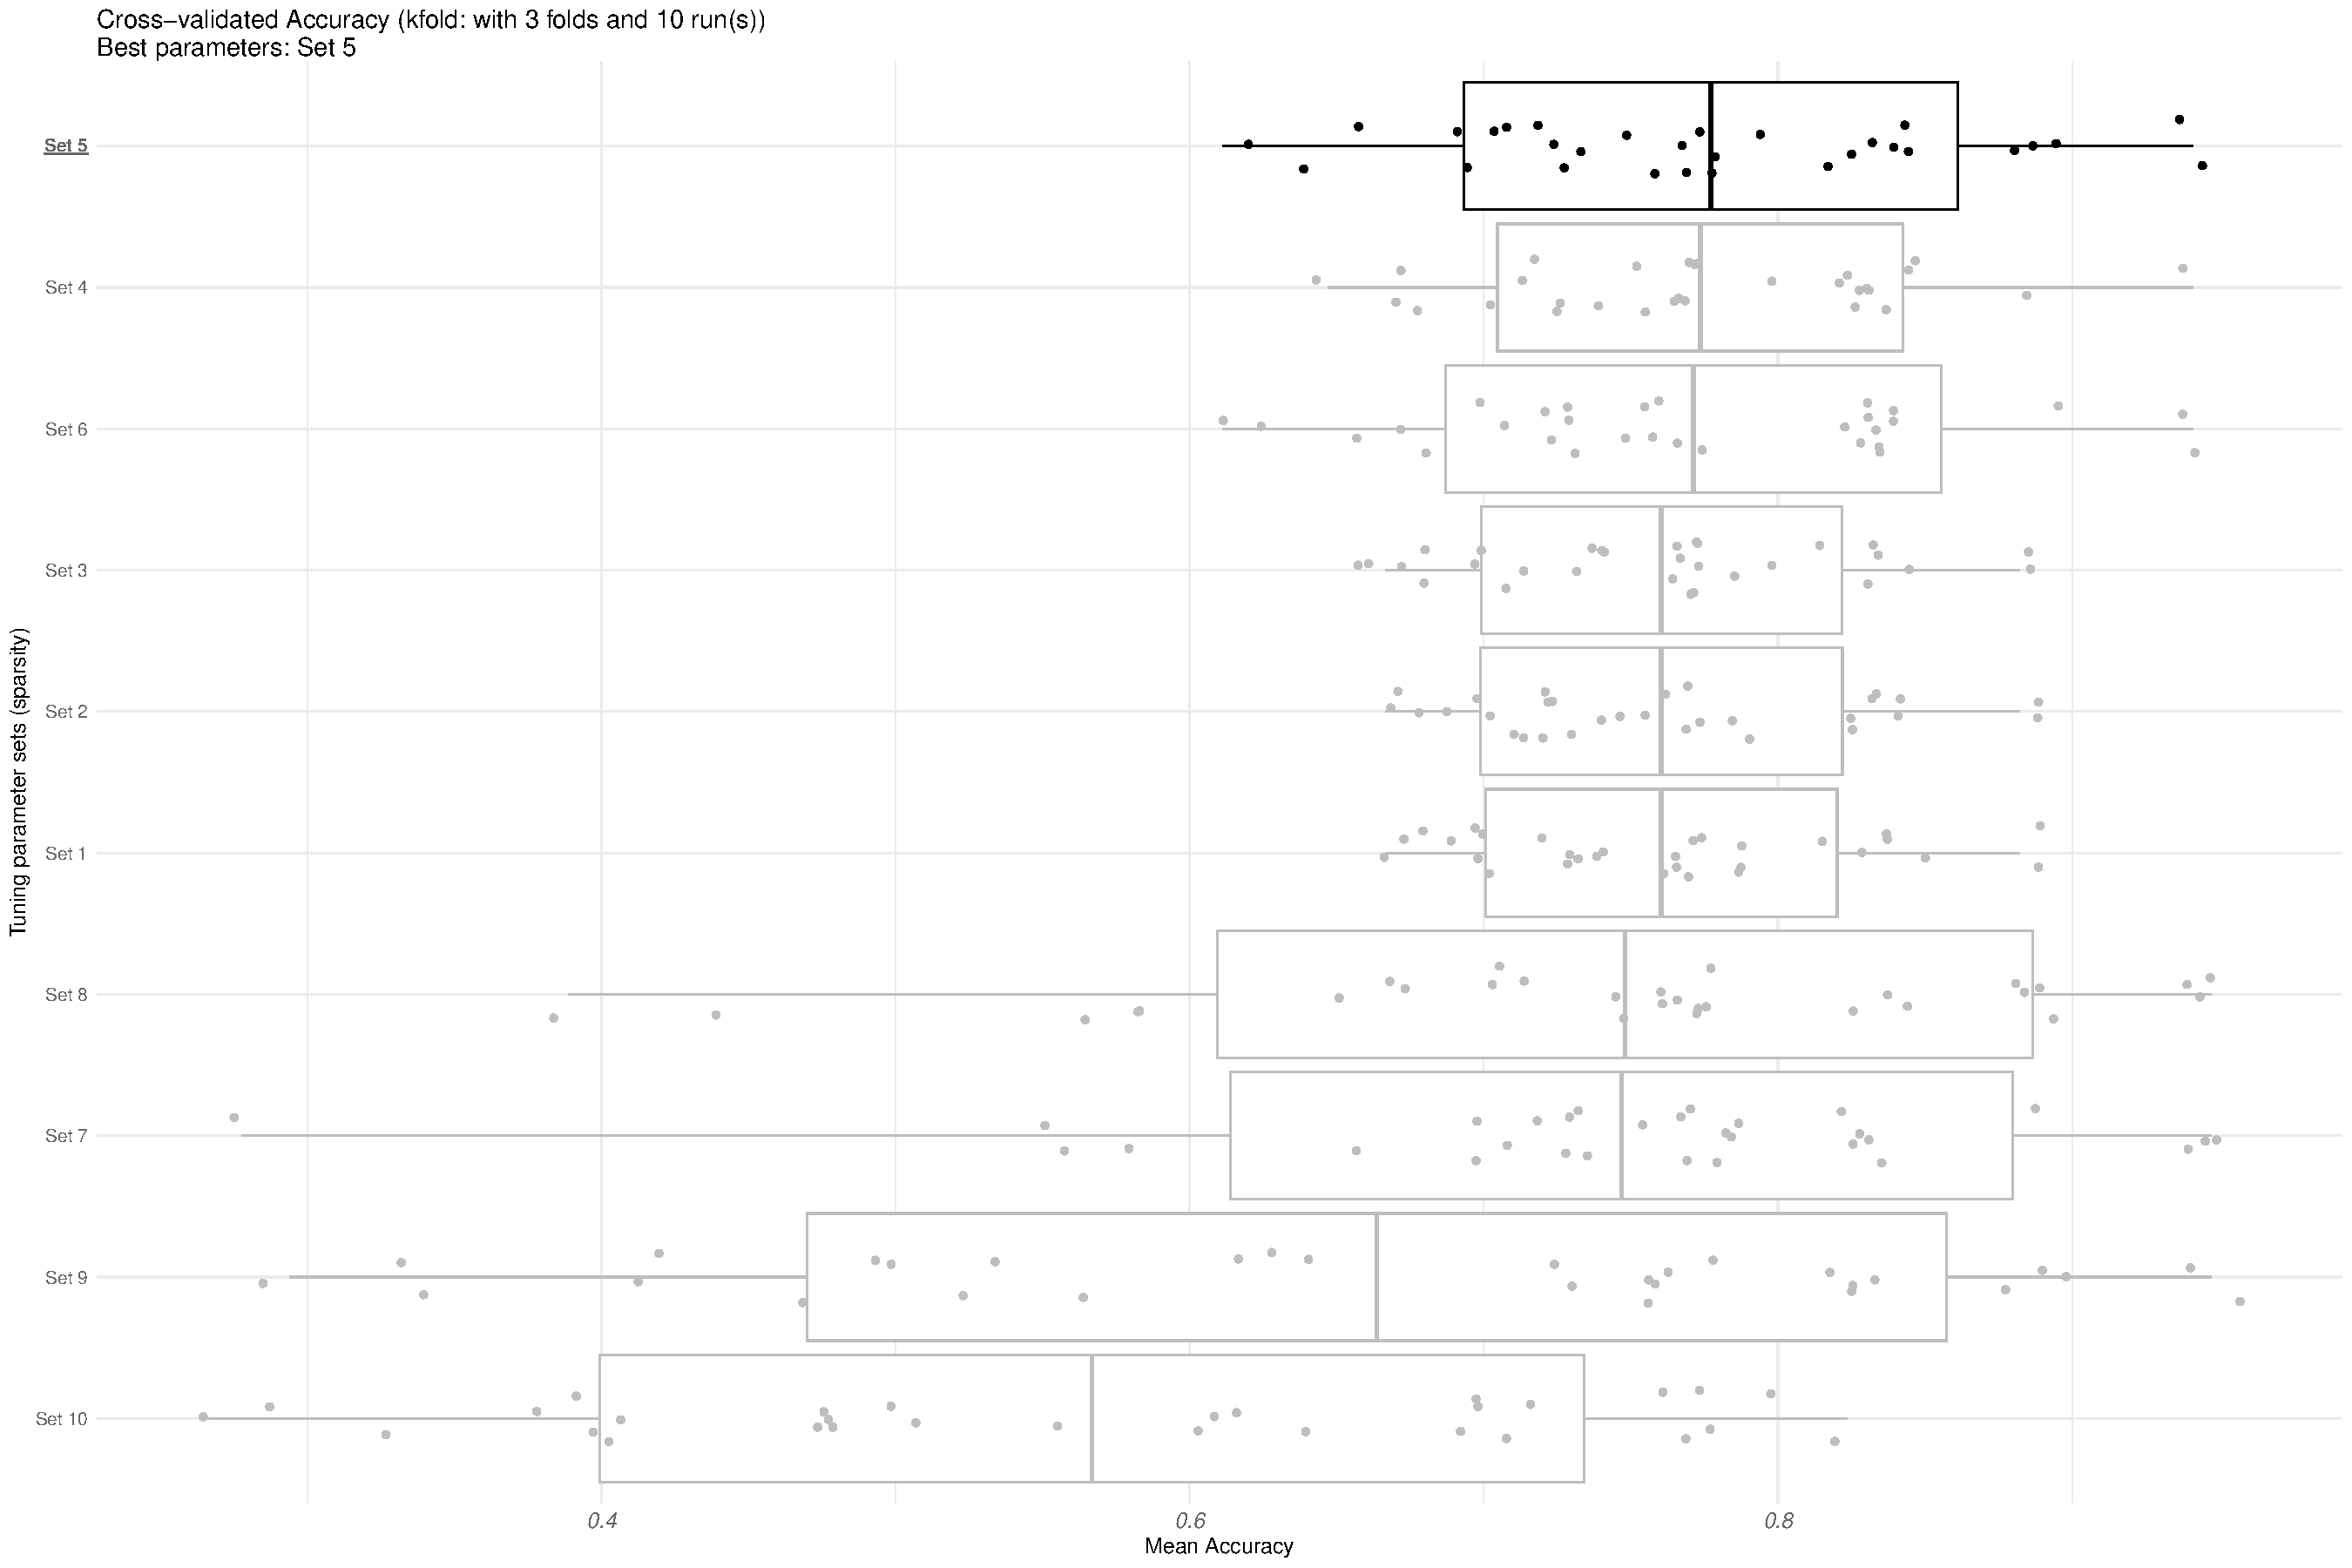
\includegraphics{RGCCA_files/figure-latex/unnamed-chunk-43-1} \end{center}

\end{CodeChunk}

\normalsize

\footnotesize

\begin{CodeChunk}
\begin{CodeInput}
R> fit = rgcca(cv_out)
\end{CodeInput}
\end{CodeChunk}

\normalsize

Notice that the sparsity parameter associated with \(\mathbf{X}_3\)
switches automatically to regularization parameter set to
\(\tau_3 = 0\). This choice is justified by the fact that we were not
looking for a block component \(\mathbf{y}_3\) that explained its own
block well (since \(\mathbf{X}_3\) is a group coding matrix) but one
that correlated with its neighboring components.

First, it possible to determine the optimal sparsity parameters by
permutation. This is made possible using the
\texttt{rgcca\_permutation()} function.

\begin{CodeChunk}
\begin{CodeInput}
R> set.seed(123456) # -> very sparse model
R> perm_out = rgcca_permutation(blocks, connection = C, response = 3,
+                                 par_type = "sparsity",
+                                 par_value = 
+                                   matrix(c(0.1, 0.25, 1, 
+                                            0.0710, 0.2000, 1,
+                                            0.0552, 0.1571, 1, 
+                                            0.0395, 0.1143, 1,
+                                            0.0237, 0.0714, 1, 
+                                            0.0080, 0.029, 1), 6, 3, 
+                                          byrow = TRUE),
+                                 n_perms = 5, n_cores = 10)
\end{CodeInput}
\end{CodeChunk}

\footnotesize

\begin{CodeChunk}
\begin{CodeInput}
R> plot(perm_out, cex = 1.3)
\end{CodeInput}


\begin{center}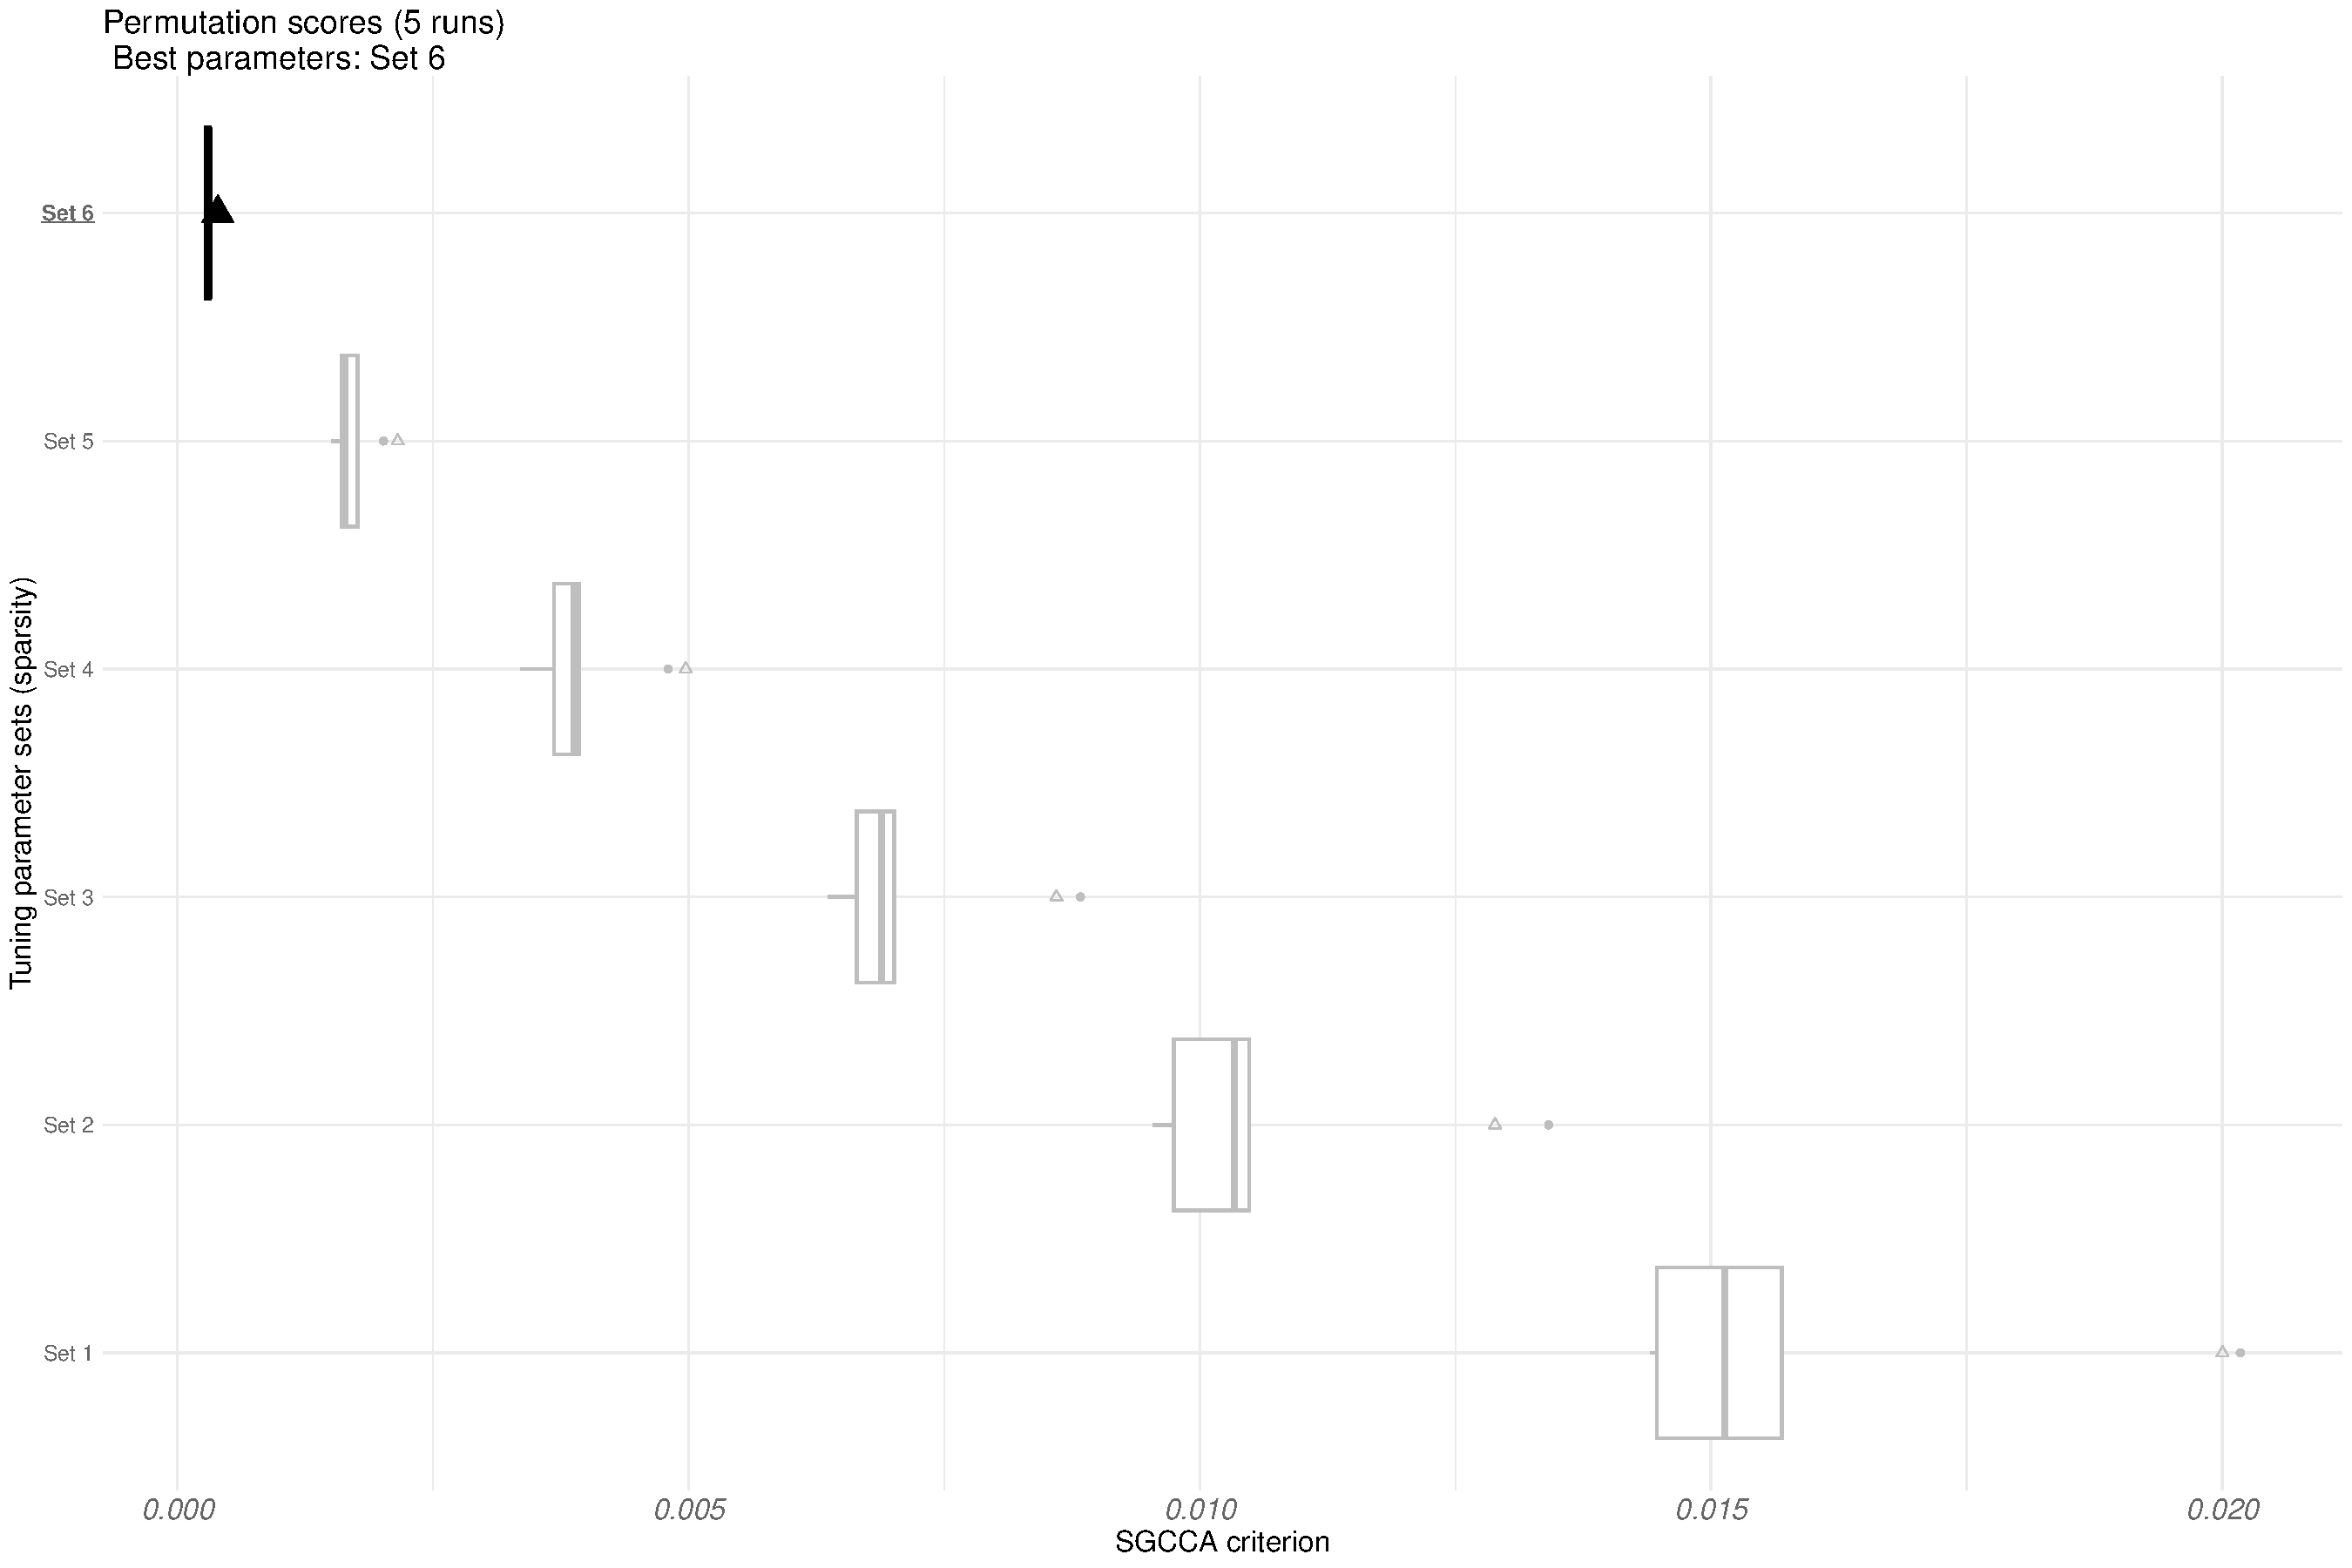
\includegraphics{RGCCA_files/figure-latex/unnamed-chunk-46-1} \end{center}

\end{CodeChunk}

\normalsize

and then directly used the optimal sparsity parameters as previously:

\footnotesize

\begin{CodeChunk}
\begin{CodeInput}
R> rgcca_opt = rgcca(perm_out)
\end{CodeInput}
\end{CodeChunk}

\normalsize

\begin{CodeChunk}
\begin{CodeInput}
R> fit_stab = rgcca_stability(rgcca_opt, 
+                            keep = sapply(rgcca_opt$a, 
+                                          function(x) mean(x!=0)),
+                            n_boot = 100, verbose = TRUE, n_cores = 15)
\end{CodeInput}
\begin{CodeOutput}
Bootstrap samples sanity check...OK
\end{CodeOutput}
\end{CodeChunk}

and then apply the bootstrap procedure on the most stable variables.

\begin{CodeChunk}
\begin{CodeInput}
R> boot_out = rgcca_bootstrap(fit_stab, n_boot = 500)
\end{CodeInput}
\begin{CodeOutput}
All the parameters were imported from the fitted rgcca_stability object.
\end{CodeOutput}
\begin{CodeOutput}
Bootstrap samples sanity check...OK
\end{CodeOutput}
\end{CodeChunk}

The bootstrap results can be visualized using the generic
\texttt{plot()} function.

\footnotesize

\begin{CodeChunk}
\begin{CodeInput}
R> plot(boot_out, block = 1:2, 
+      display_order = FALSE, 
+      n_mark = 2000, cex = 1.3)
\end{CodeInput}


\begin{center}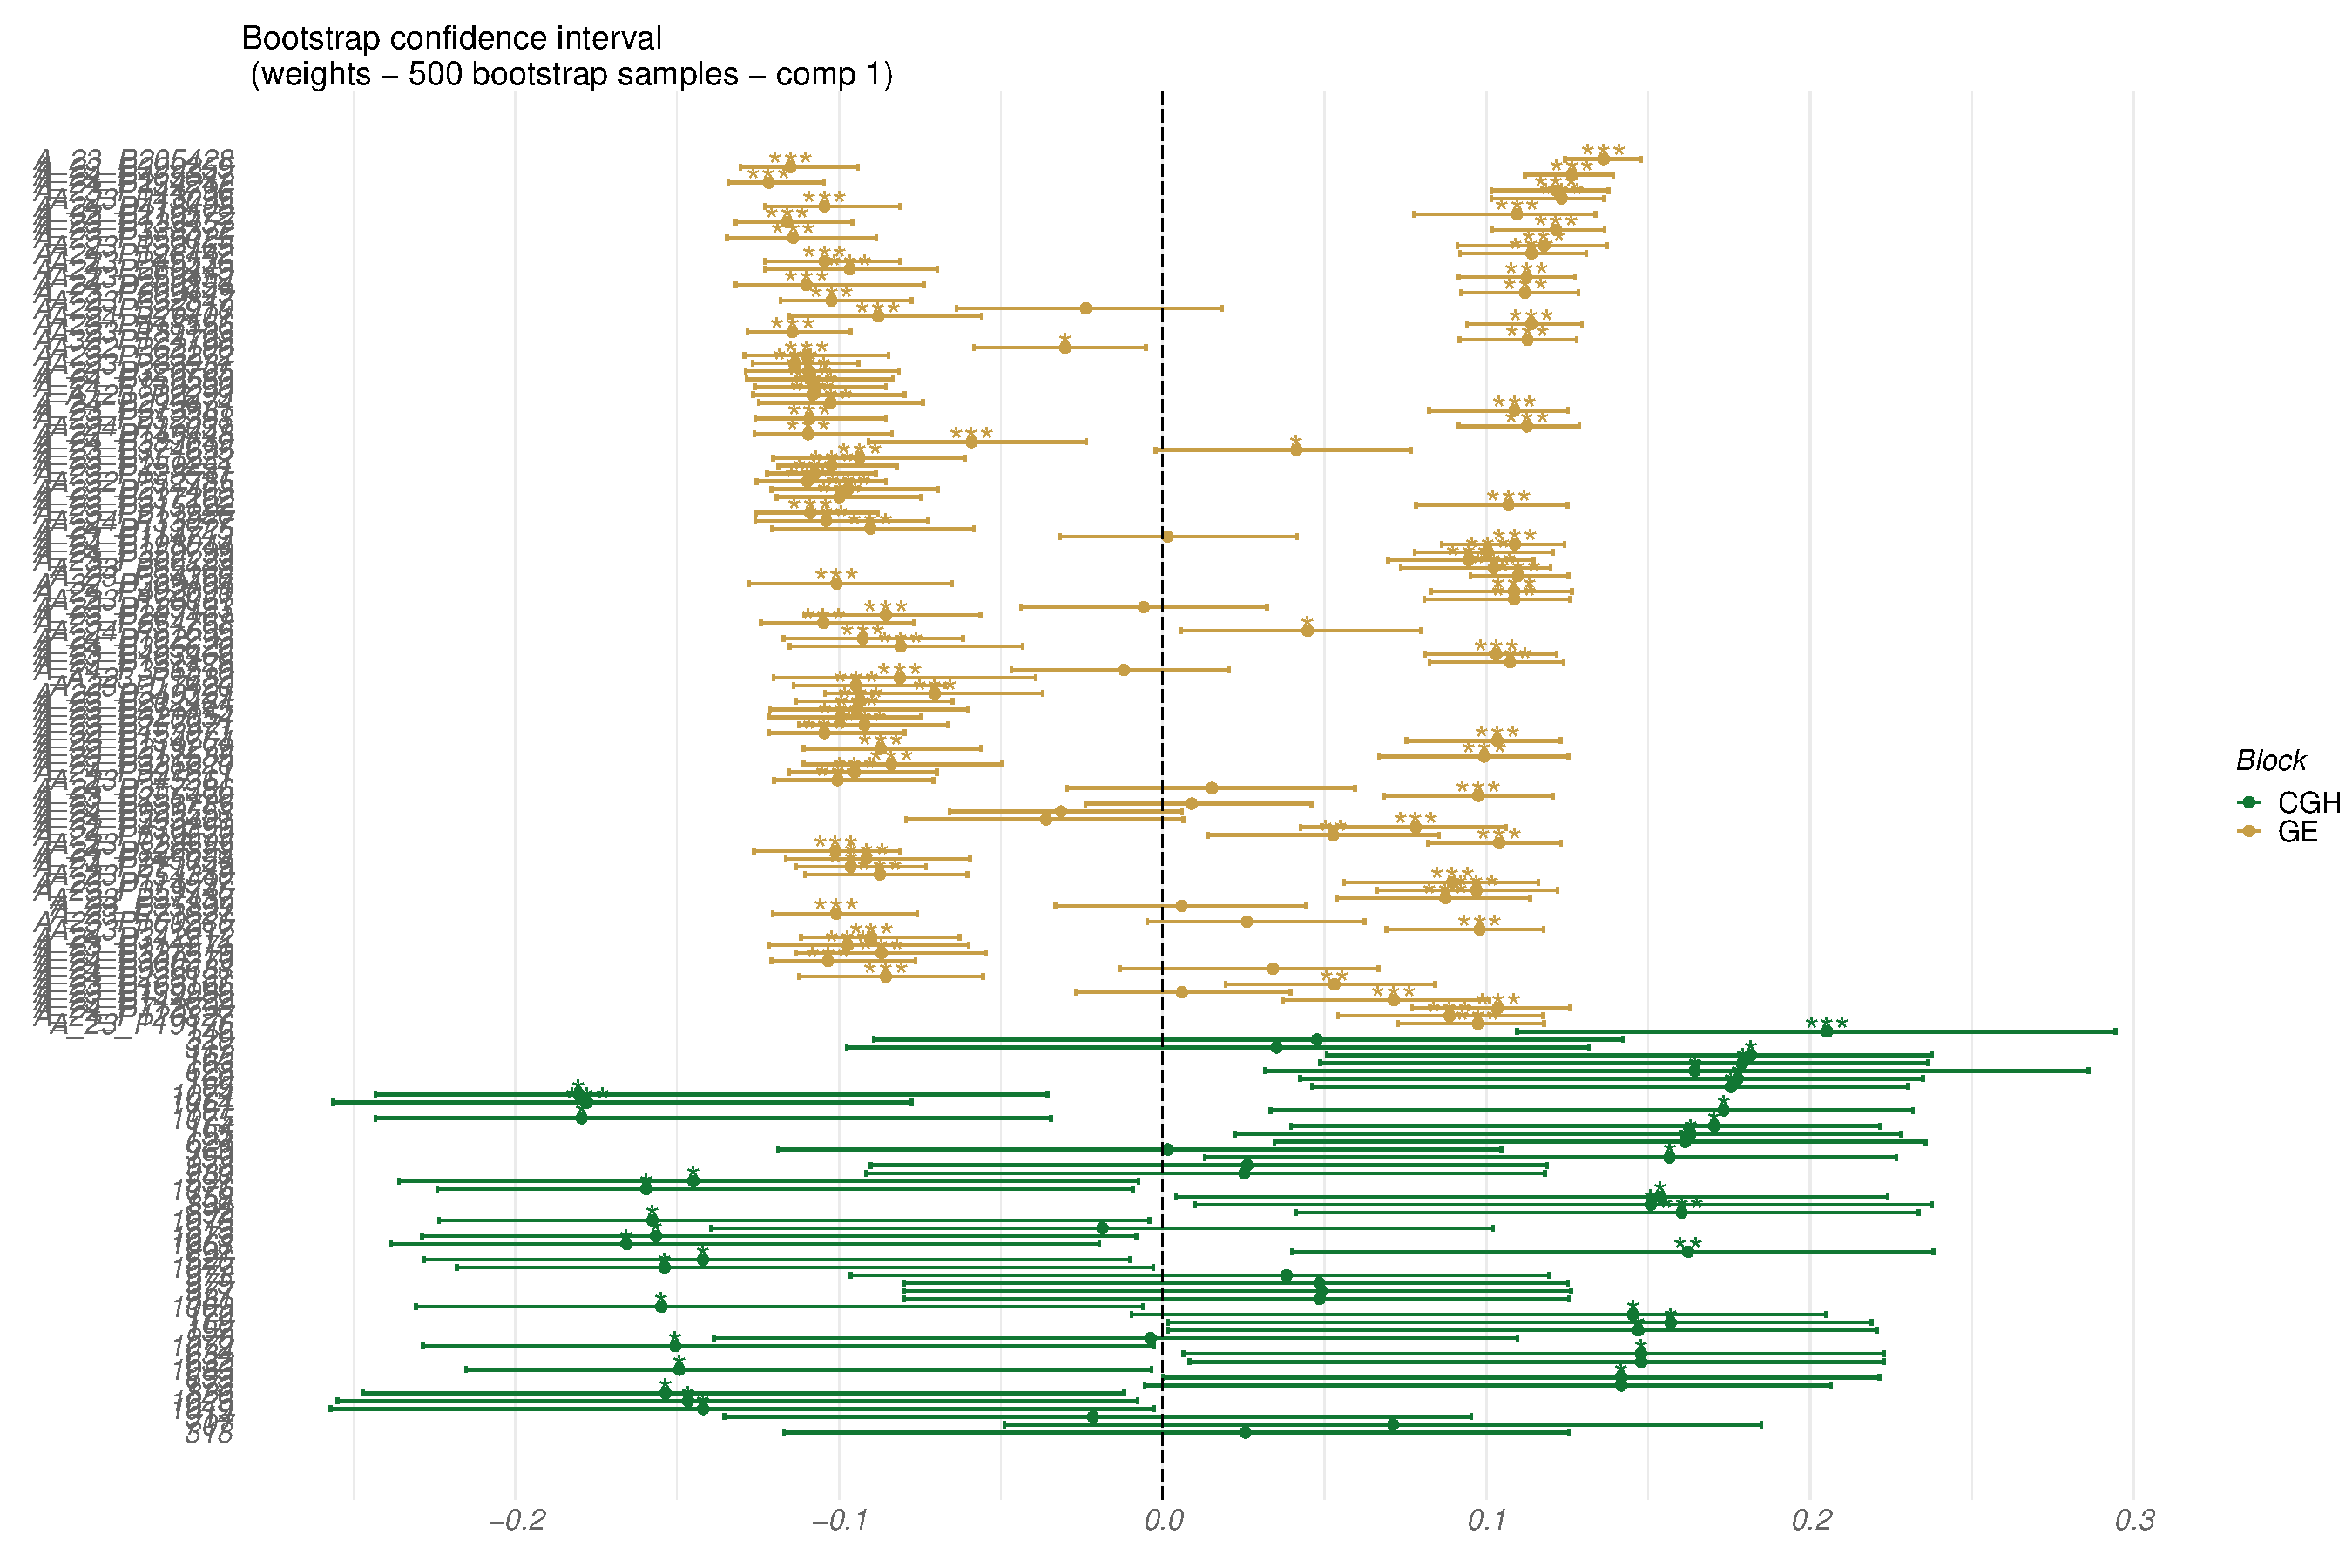
\includegraphics{RGCCA_files/figure-latex/unnamed-chunk-50-1} \end{center}

\end{CodeChunk}

\normalsize

One component per block has been built (GE1 for \(\mathbf{X}_1\) and
CGH1 \(\mathbf{X}_2\)), and the graphical display of the tumors obtained
by crossing GE1 and CGH1 and labeled according to their location is
shown below.

\footnotesize

\begin{CodeChunk}
\begin{CodeInput}
R> plot(fit_stab$rgcca_res, type = "sample", block=1:2, 
+      comp=1, resp = as.character(Loc), 
+      cex = 1.3
+      )
\end{CodeInput}
\begin{figure}

{\centering 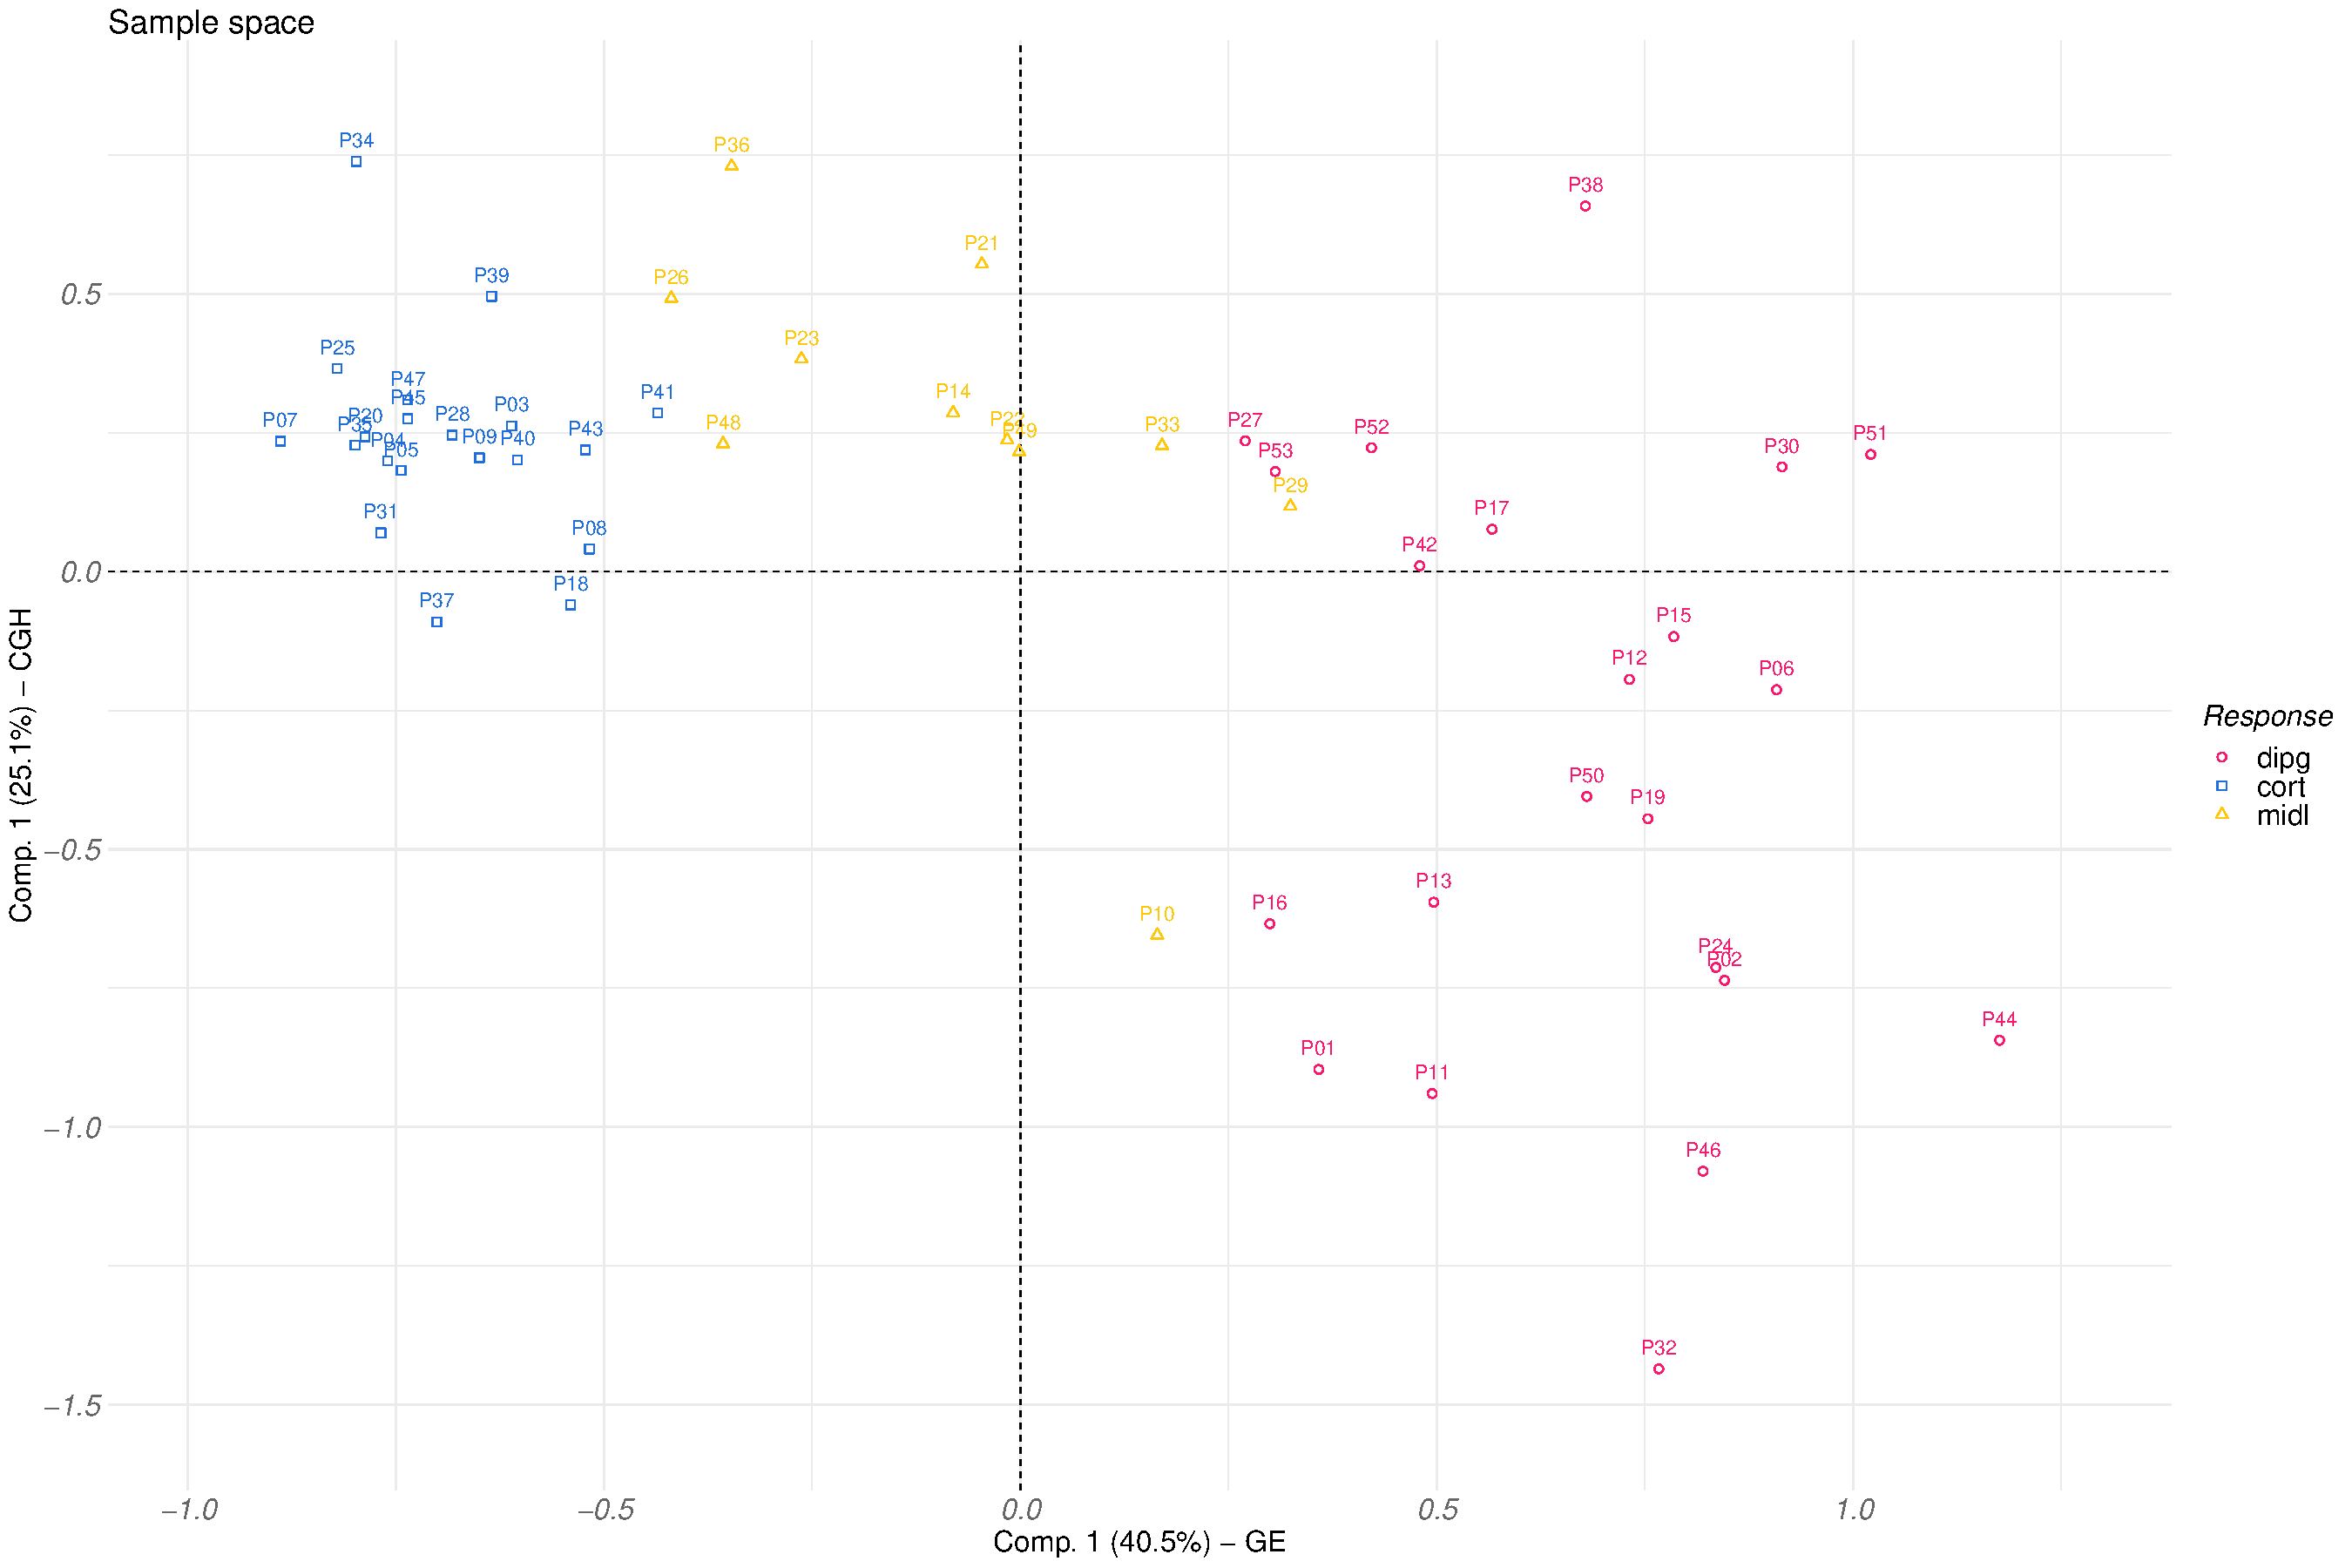
\includegraphics{RGCCA_files/figure-latex/unnamed-chunk-51-1} 

}

\caption[graphical display of the tumors obtained by crossing GE1 and CGH1 and labeled according to their location]{graphical display of the tumors obtained by crossing GE1 and CGH1 and labeled according to their location.}\label{fig:unnamed-chunk-51}
\end{figure}
\end{CodeChunk}

\normalsize

We observe that \texttt{GE} contains much more discriminative
information than \texttt{CGH}. \newpage

\hypertarget{conclusion}{%
\section{Conclusion}\label{conclusion}}

This package gathers 60 years of multiblock component methods and offers
a unified implementation strategy for these methods. This release of the
RGCCA package includes:

\begin{itemize}
\item
  Special attention has been paid to recover the results of other R
  packages of the literature including \texttt{ade4} and
  \texttt{factomineR} and \texttt{mixOmics}.
\item
  K-fold cross-validation and permutation based strategies for optimal
  choice of the shrinkage parameters/level of sparsity.
\item
  a bootstrap resampling procedure for assessing the reliability of the
  parameters estimates of S/RGCCA.
\item
  Dedicated functions for graphical representations of the ouptut of
  RGCCA (sample plot, correlation circle, etc\ldots).
\item
  multiblock data faces two types of missing data structure: (i) if an
  observation \(i\) has missing values on a whole block j and (ii) if an
  observation i has some missing values on a block j (but not all). For
  these two situations, it is possible to exploit the algorithmic
  solution proposed for PLS path modeling to deal with missing data (see
  \citep{Tenenhaus2005}, page 171).
\end{itemize}

At last, RGCCA for multigroup data \citep{Tenenhaus2014b} and for RGCCA
for multiway data \citep{Gloaguen2020} has been proposed but not yet
integrated in the RGGCA package. In addition, global RGCCA has been
recently developed and enables extracting simultaneously several
components per block (no deflation procedure required). Work in progress
includes the integration of this novel procedures in the next release of
the package.

\renewcommand\refname{References}
\bibliography{biblio.bib}



\end{document}
